\chapter{Unsupervised Learning and Large Scale Problems}
\section{Exercises}
\subsection{Kernel principal component analysis}
\textbf{Describe how you can do denoising using PCA. Describe what happens with the denoising if you increase the number of principal components.}

PCA is a technique that transforms and maps the observations to a lower dimension space such that the greatest variance by some scalar projection of the data lies on the first coordinate (called the first principal component), the second greatest variance on the second coordinate, and so on. The projections or the principal components is meant to have only the relevant features of the data. Therefore, PCA can be used for the purpose of denoising where the components are expected to have only the data features and not the noise. PCA does a linear orthogonal transformation and therefore cannot handle complex or non-linear data patterns. This motivates us to  use a kernel PCA which can handle non-linear features. In the provided kpca script we use an example dataset with 400 points and noise has been added. To denoise the original data from the noisy one, we use (1;2;3;7;11;15) principal components. The model performance is shown in figure \ref{fig:pca_nc}. It can be observed from the figure \ref{fig:pca_nc} that as the number of principal components increases, more information is retained during the denoising and it becomes close to the actual data.
\begin{figure}[ht]
	\centering
	\begin{subfigure}[b]{0.32\textwidth}
		\centering
		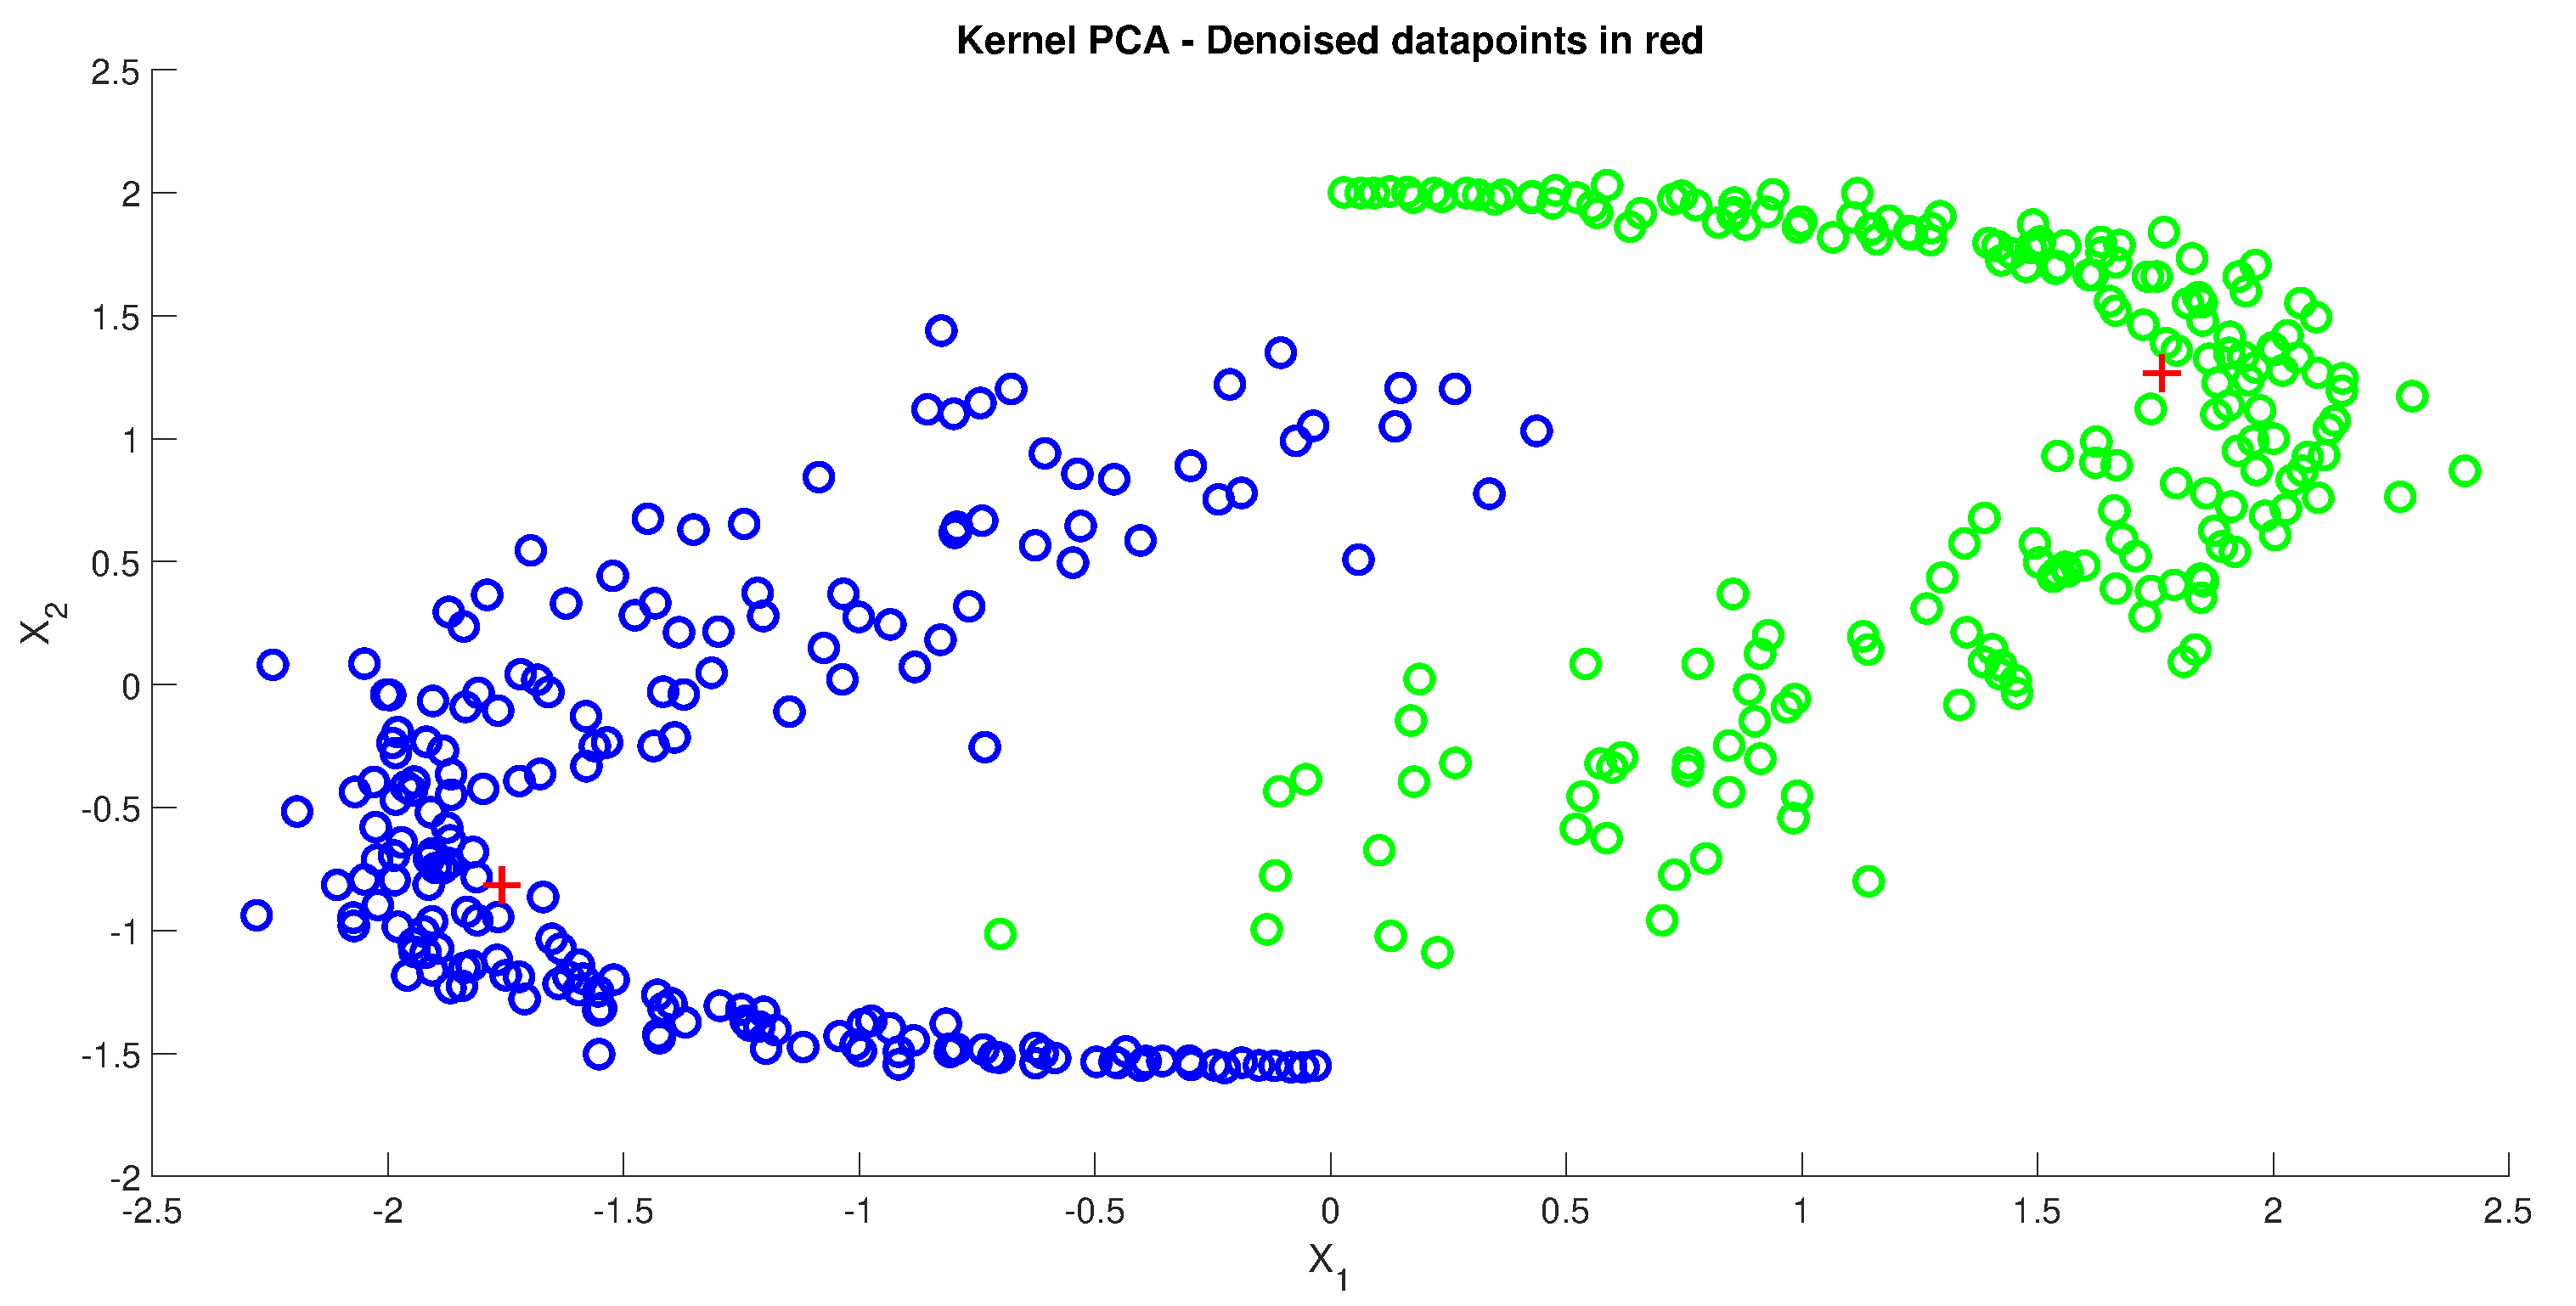
\includegraphics[width = 0.85\textwidth]{Exercise3/Report/pca_nc_1}
		\caption{kpca components = 1 }\label{fig:pca_nc_1}3
	\end{subfigure}%
	\begin{subfigure}[b]{0.32\textwidth}
		\centering
		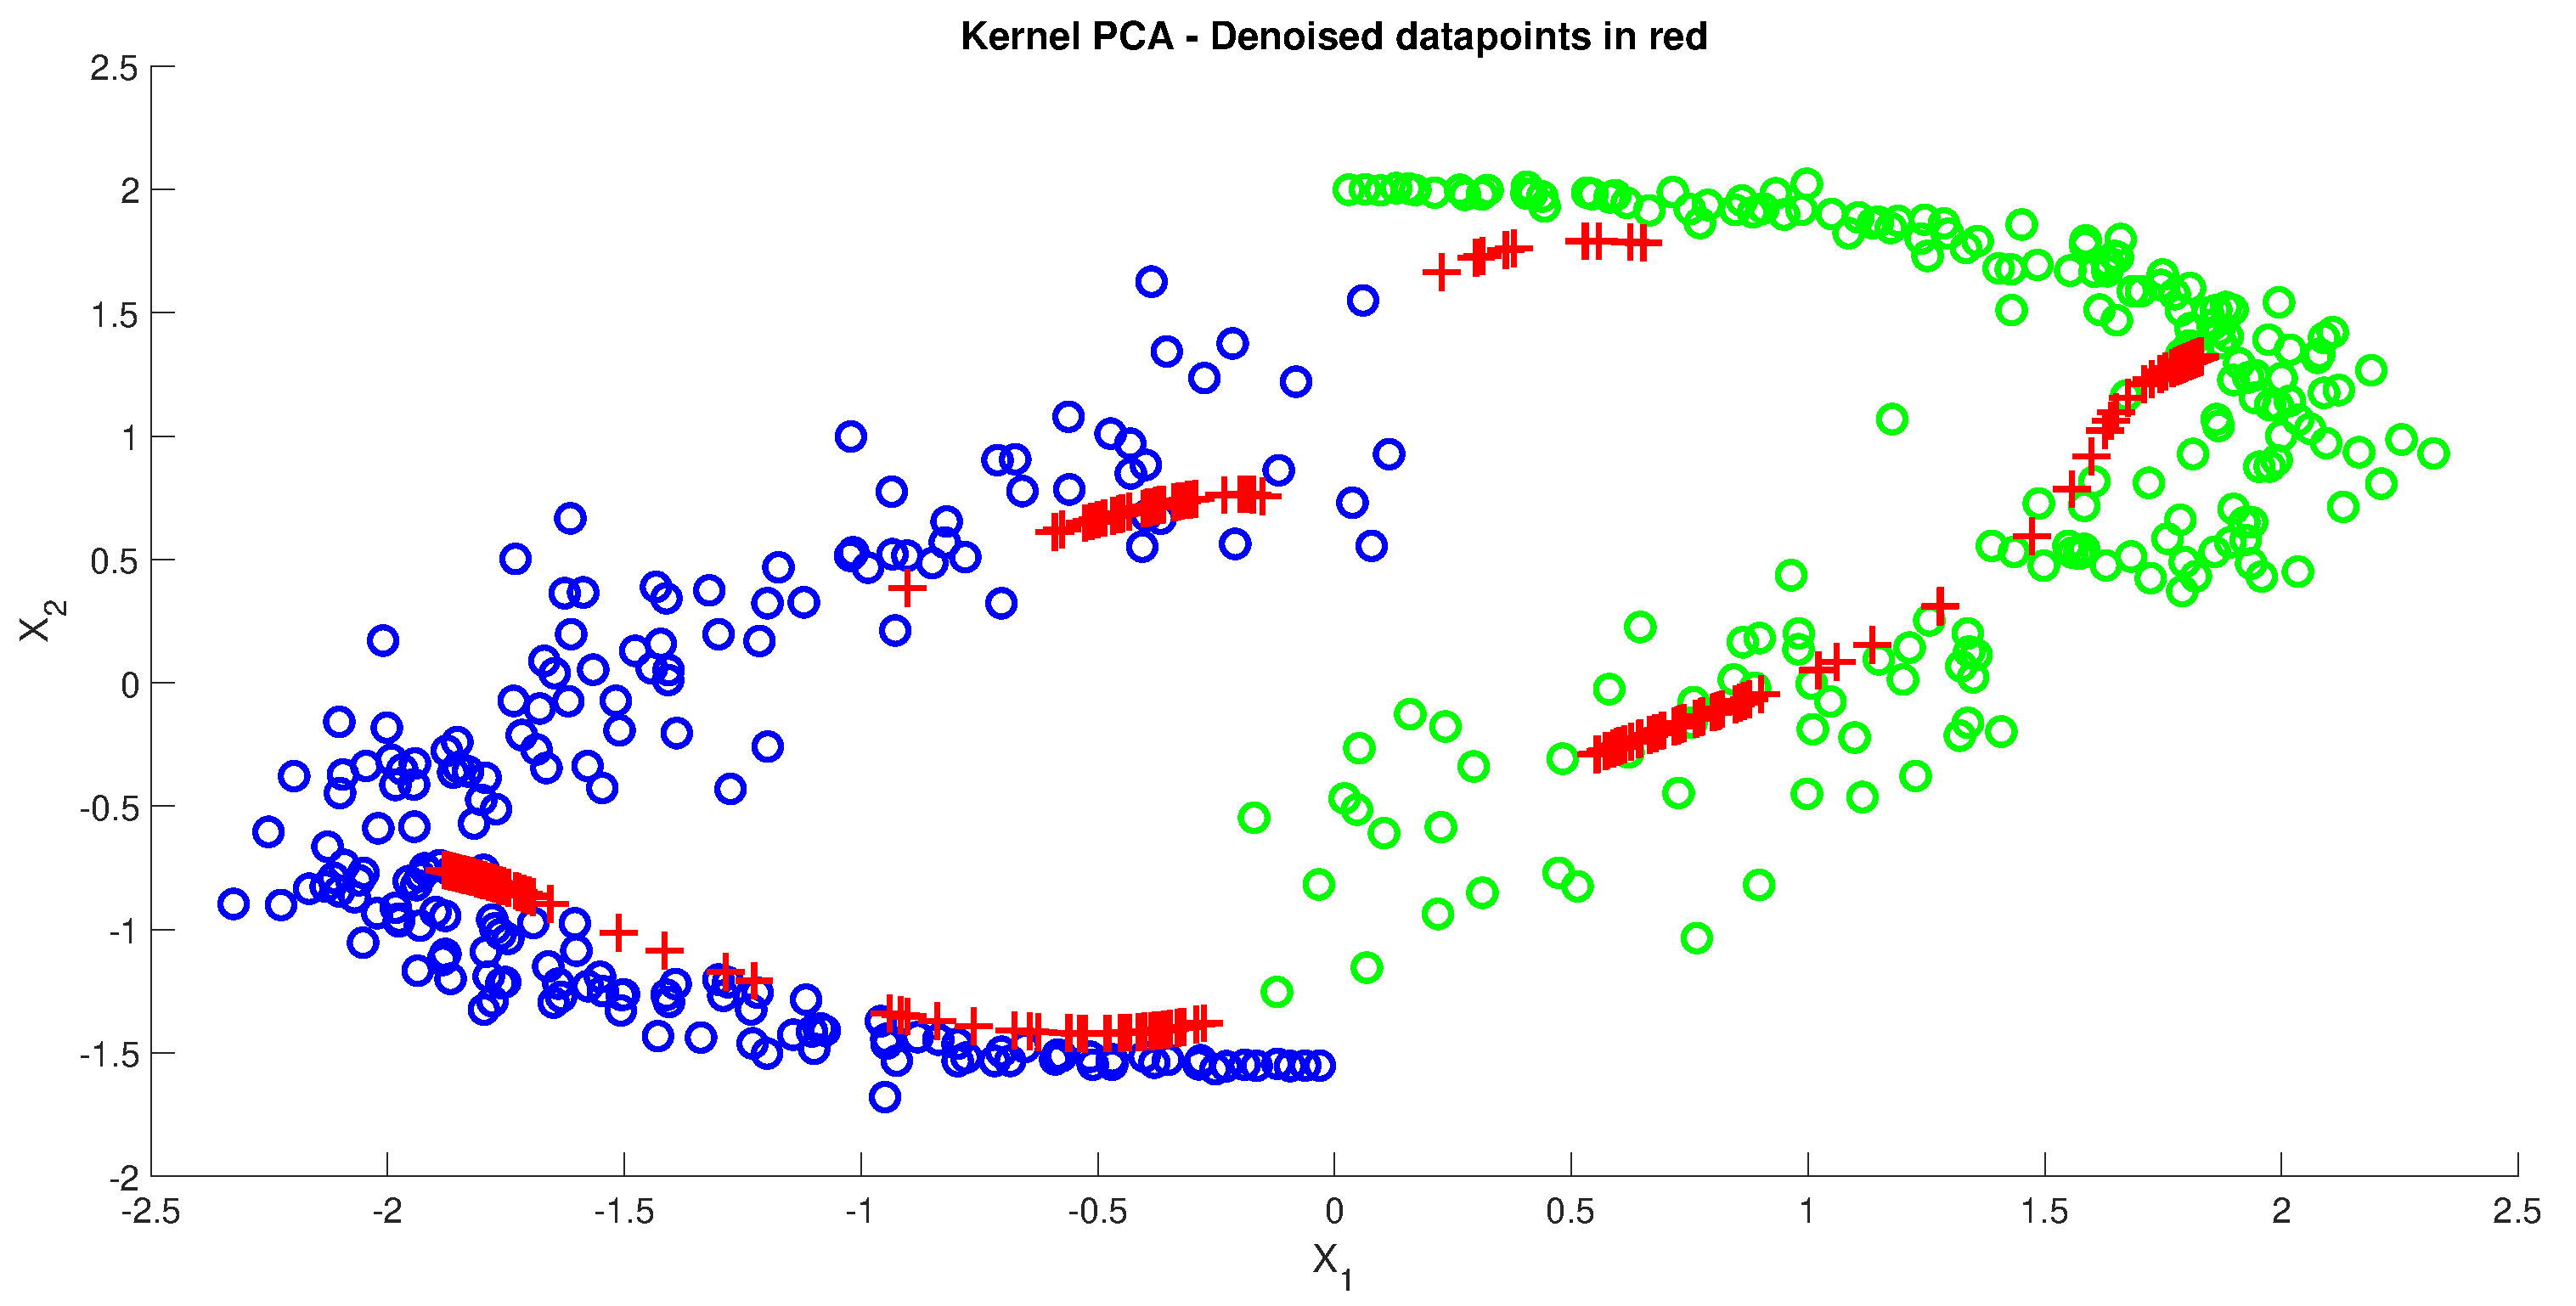
\includegraphics[width = 0.85\textwidth]{Exercise3/Report/pca_nc_2}
		\caption{kpca components = 2}\label{fig:pca_nc_2}
	\end{subfigure}%
	\begin{subfigure}[b]{0.32\textwidth}
		\centering
		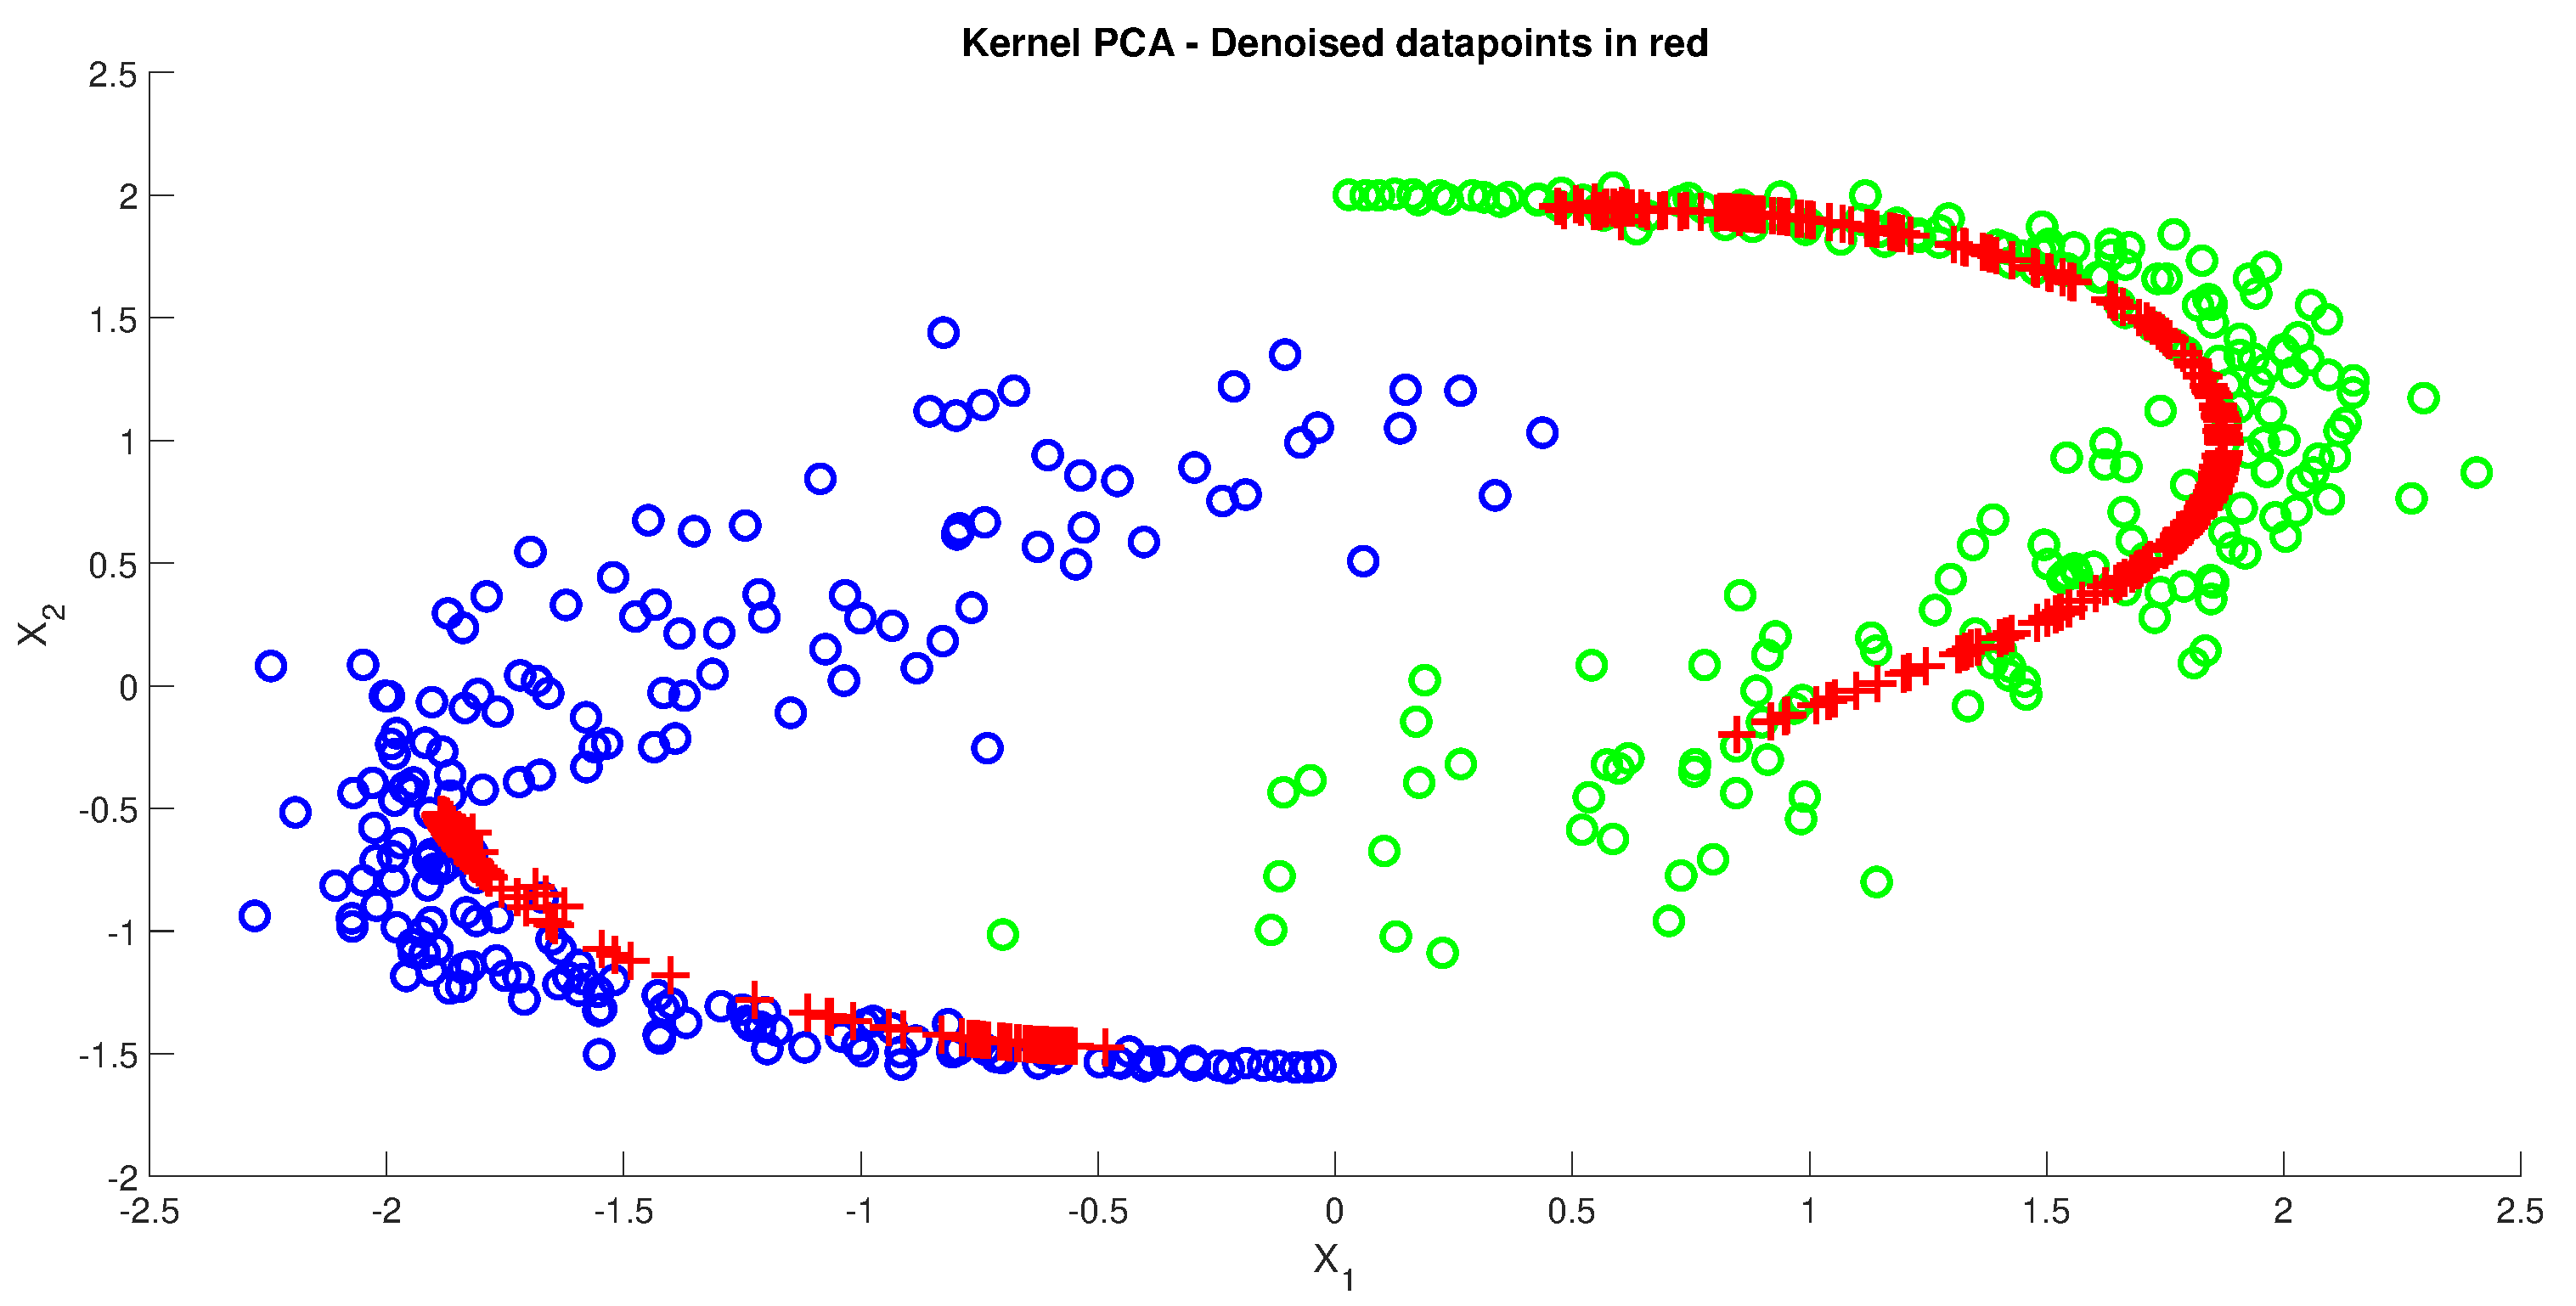
\includegraphics[width = 0.85\textwidth]{Exercise3/Report/pca_nc_3}
		\caption{kpca components = 3 }\label{fig:pca_nc_3}
	\end{subfigure}
	\begin{subfigure}[b]{0.32\textwidth}
		\centering
		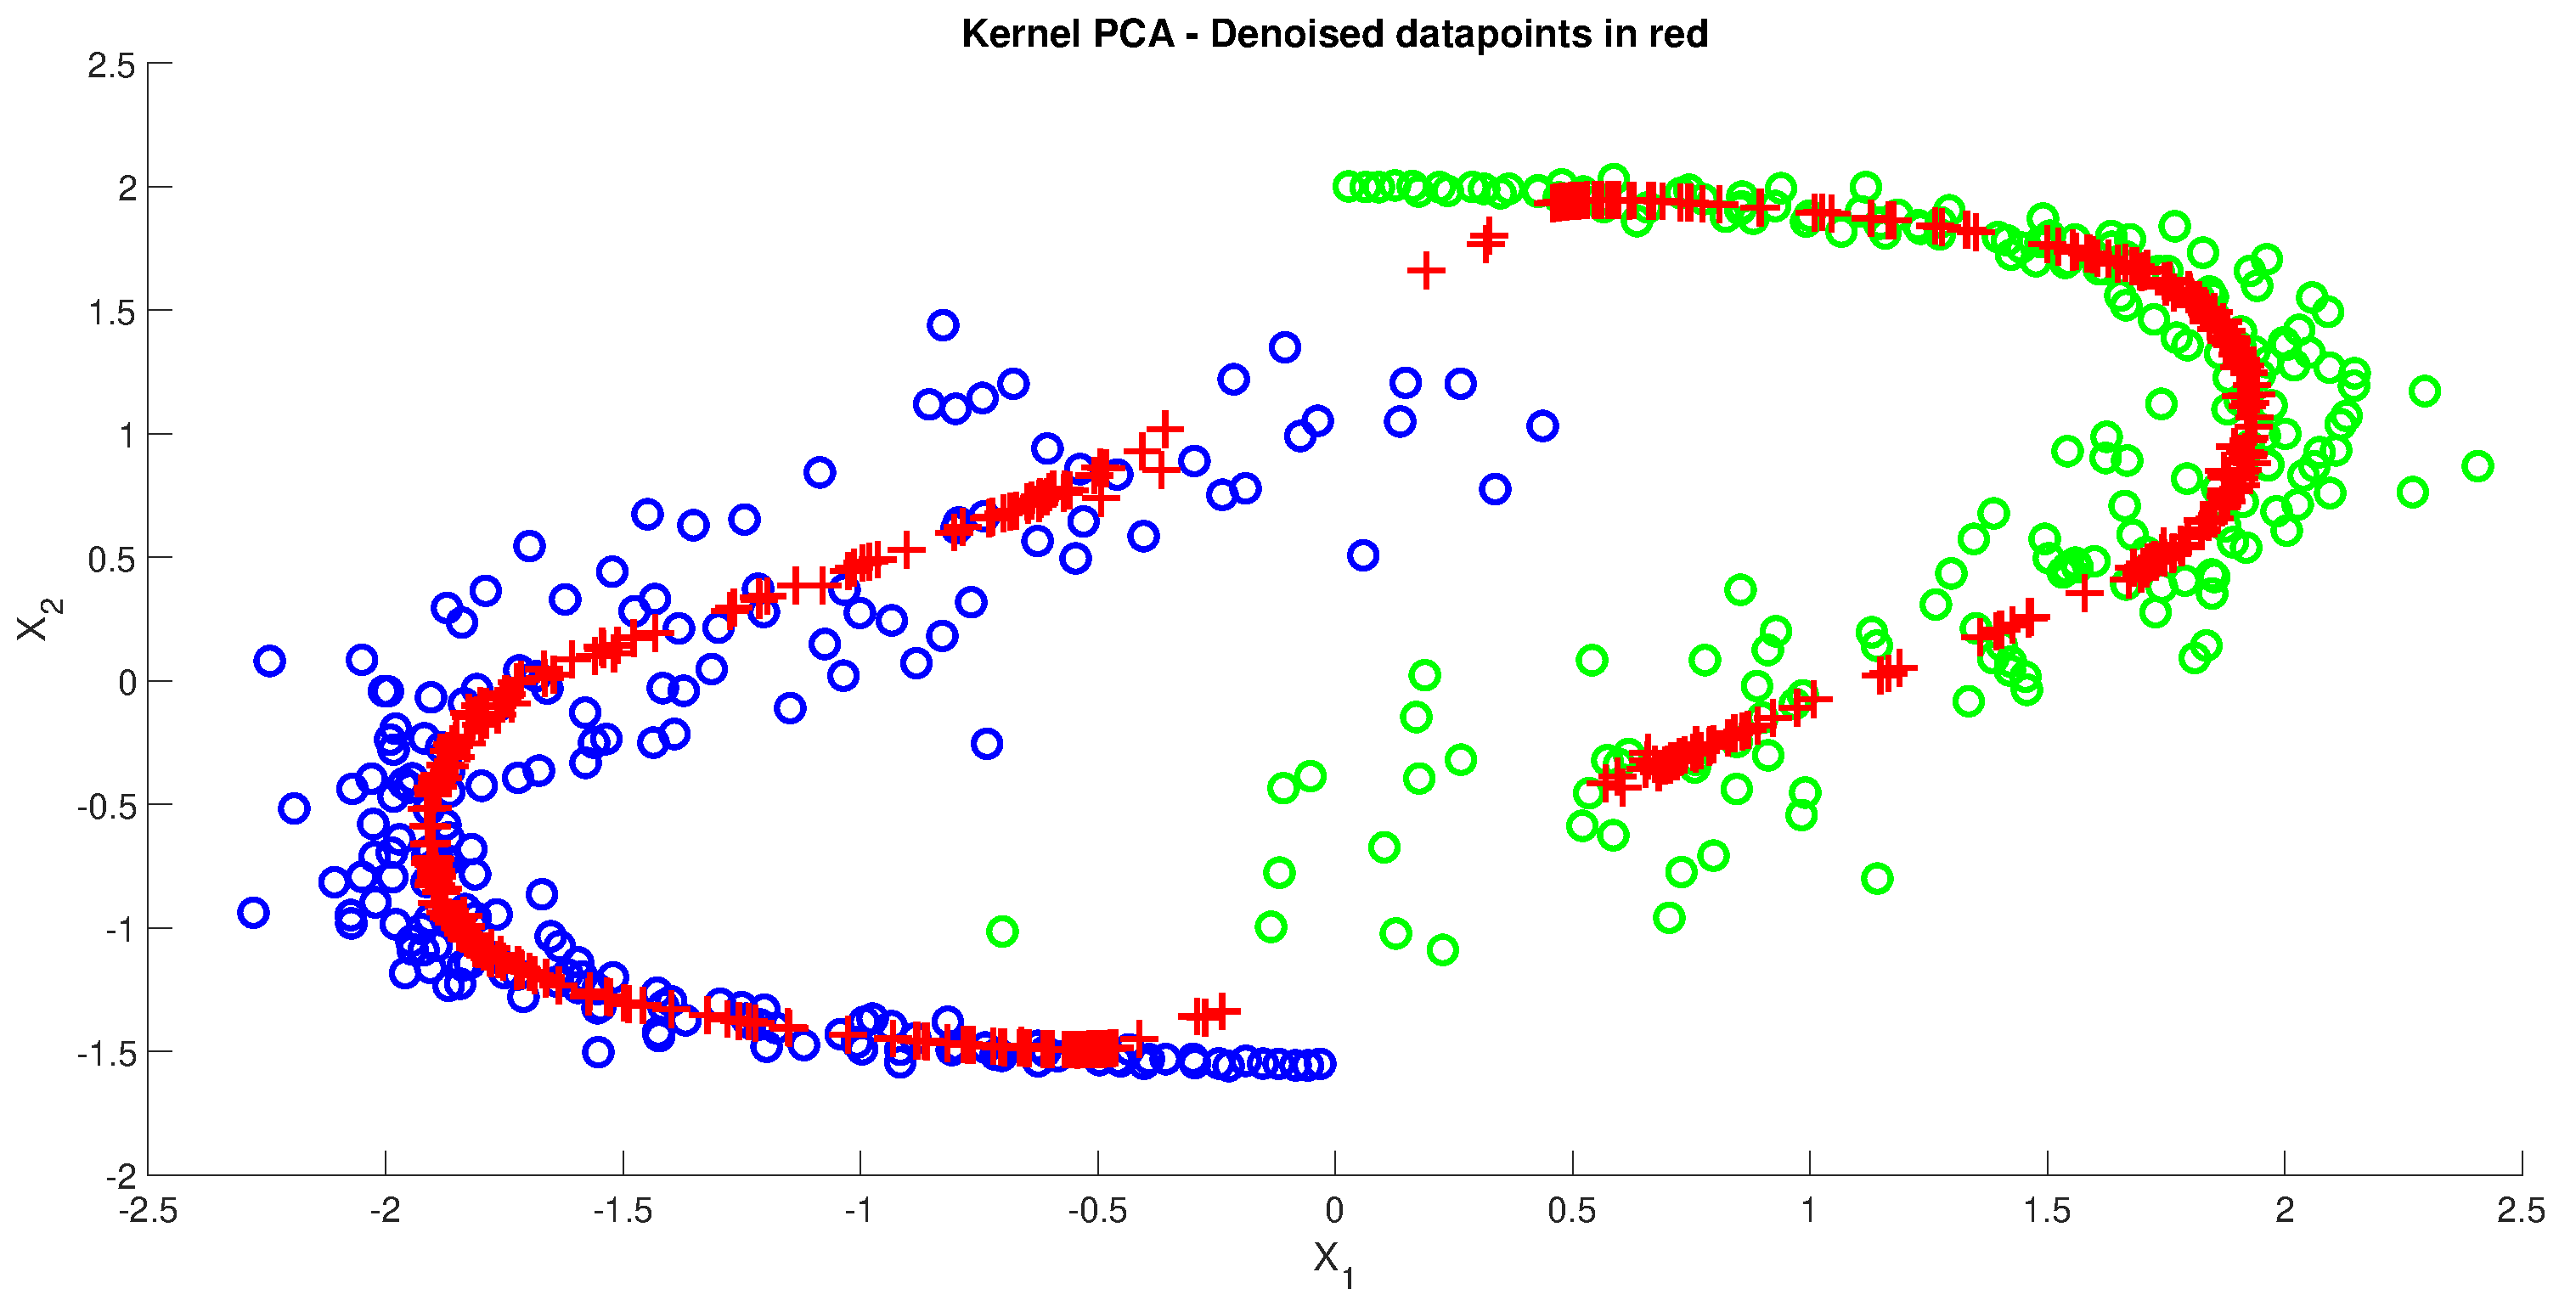
\includegraphics[width = 0.85\textwidth]{Exercise3/Report/pca_nc_7}
		\caption{kpca components = 7 }\label{fig:pca_nc_7}
	\end{subfigure}%
	\begin{subfigure}[b]{0.32\textwidth}
		\centering
		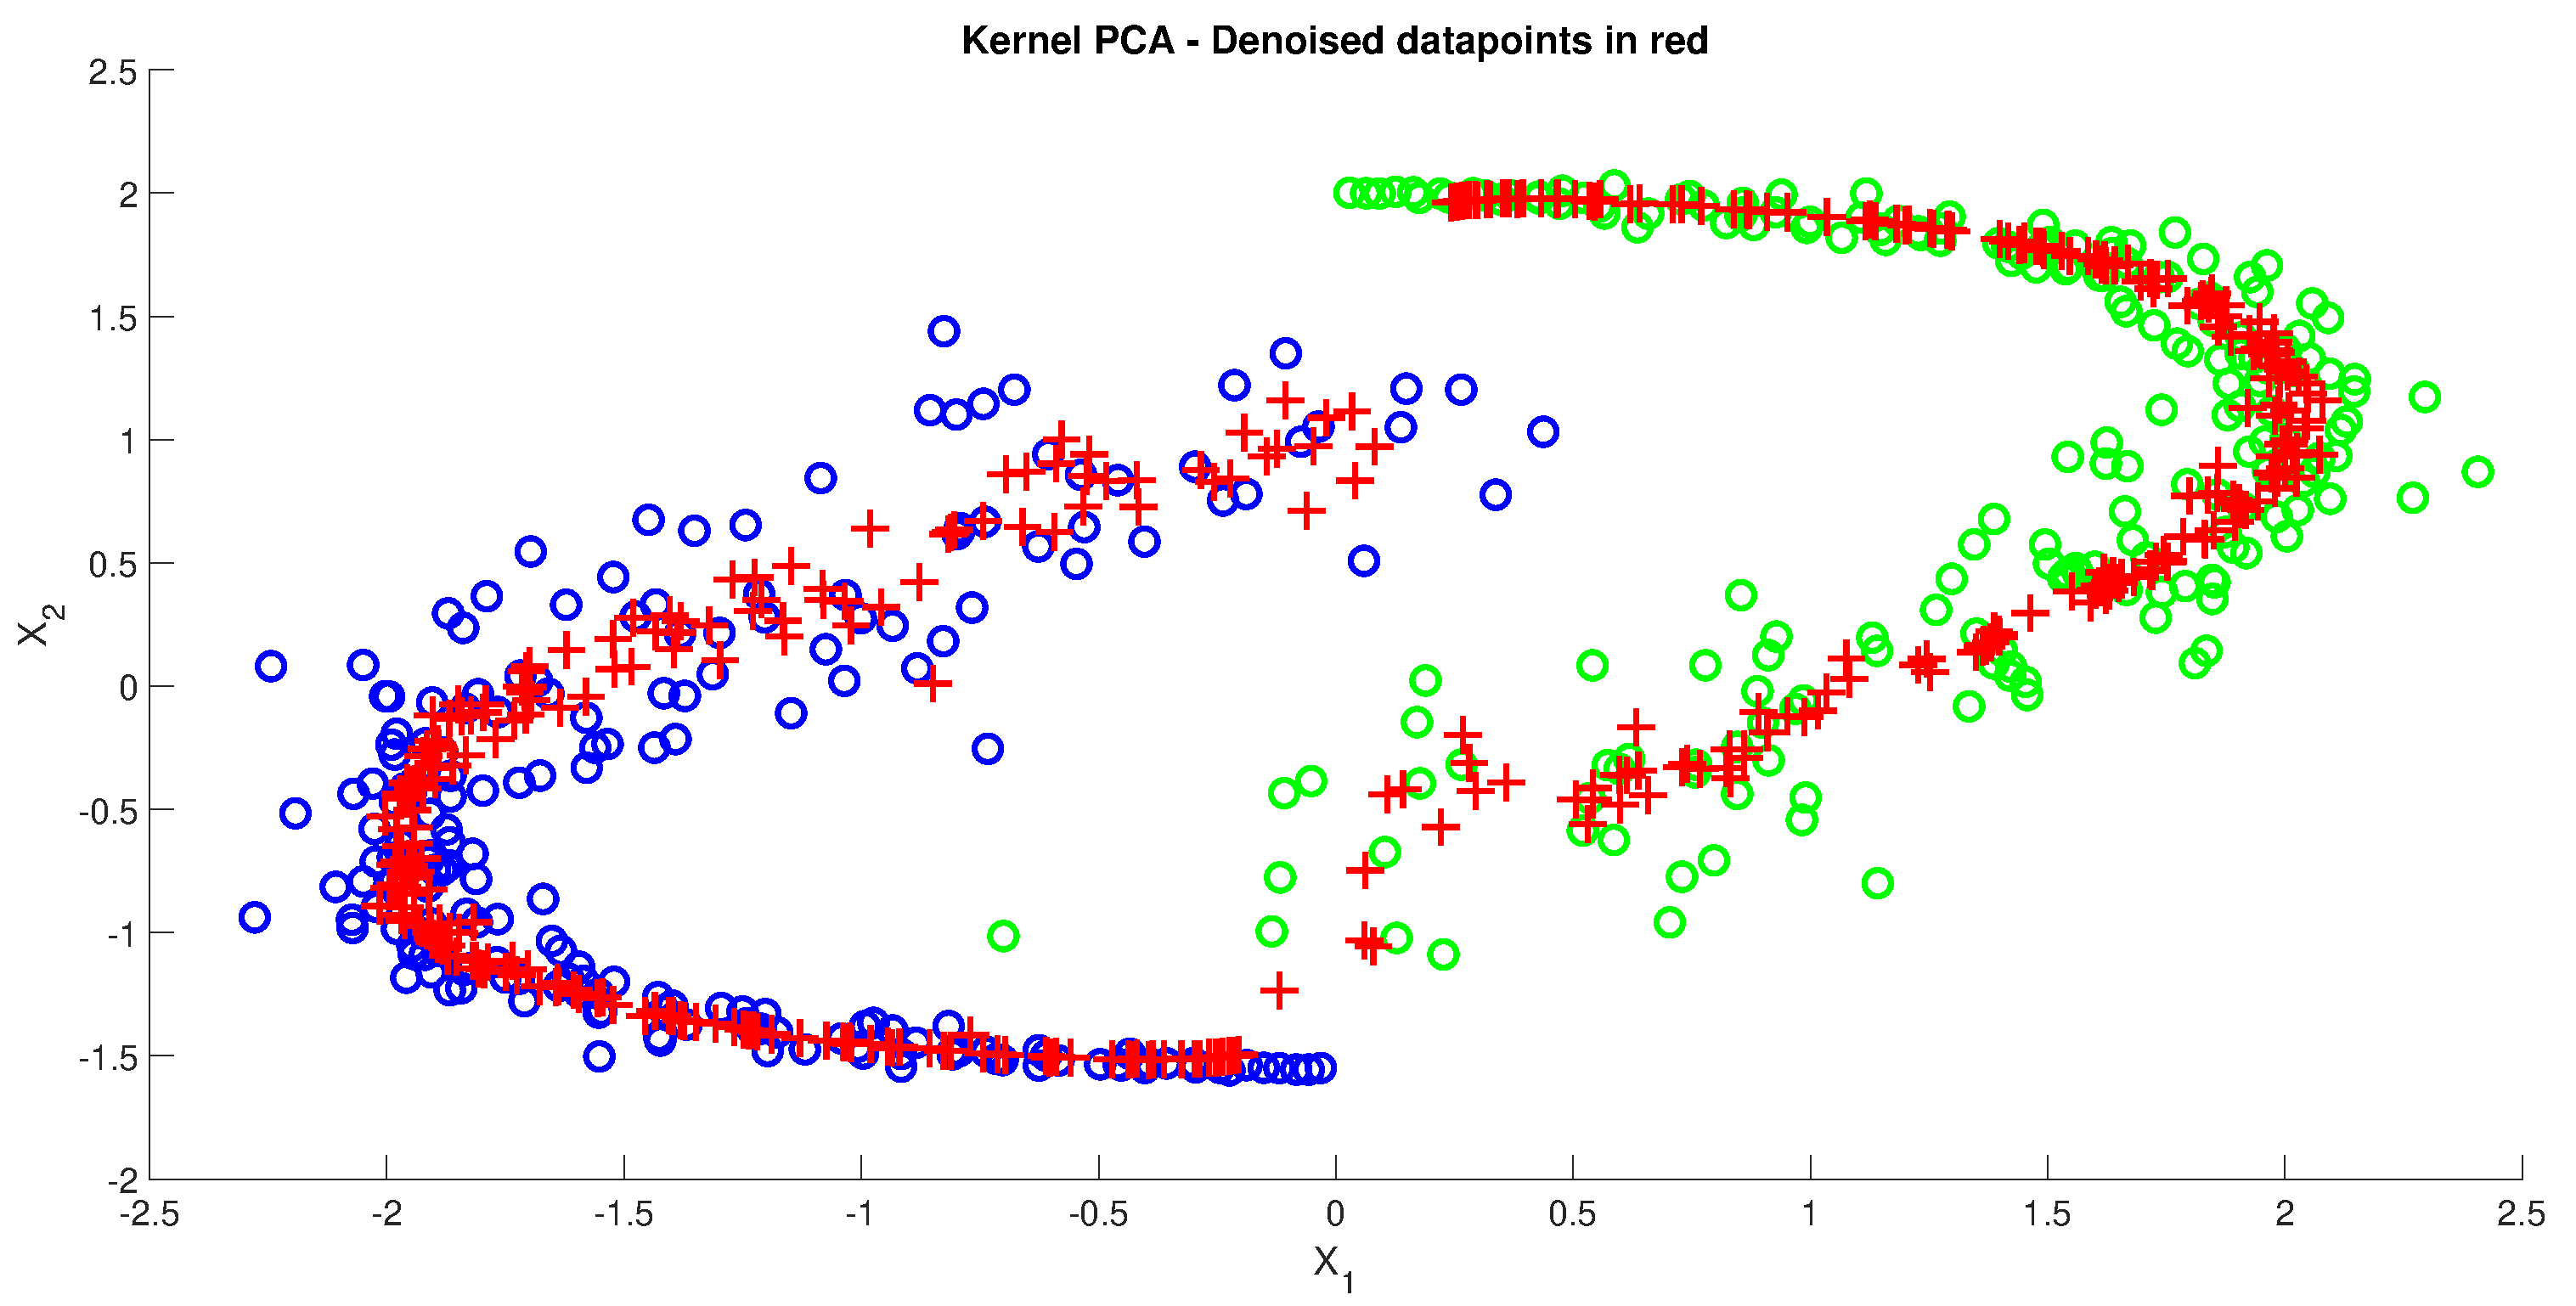
\includegraphics[width = 0.85\textwidth]{Exercise3/Report/pca_nc_11}
		\caption{kpca components = 11 }\label{fig:pca_nc_11}
	\end{subfigure}%
	\begin{subfigure}[b]{0.32\textwidth}
		\centering
		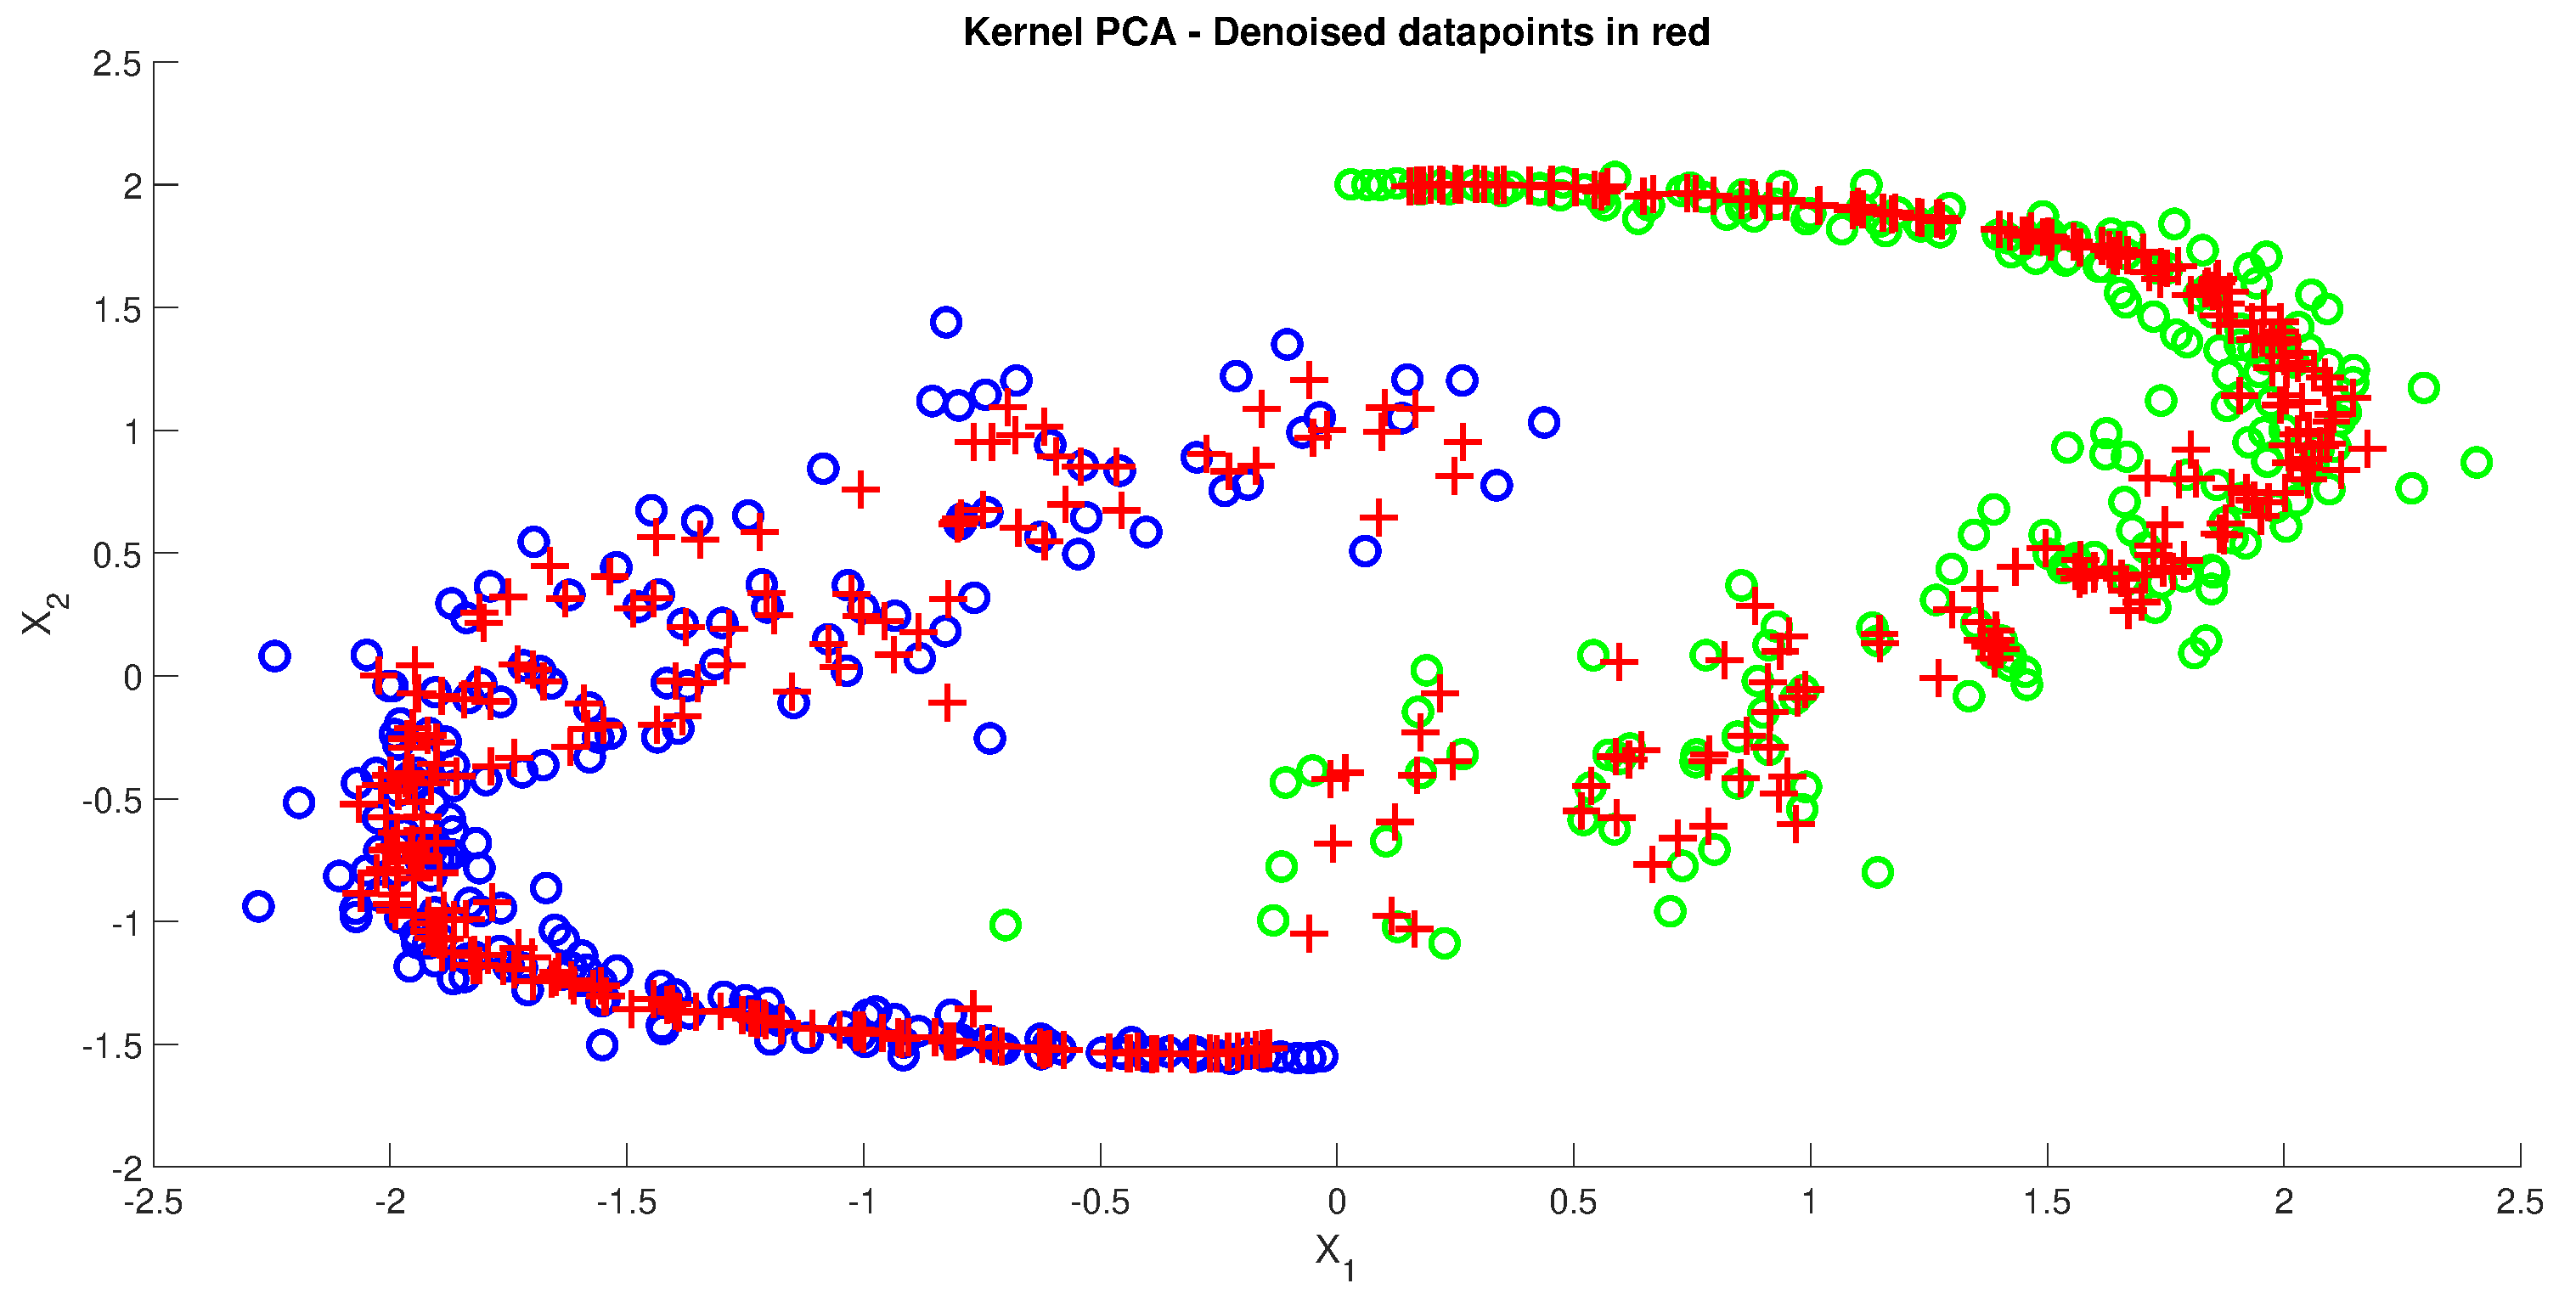
\includegraphics[width = 0.85\textwidth]{Exercise3/Report/pca_nc_15}
		\caption{kpca components = 15}\label{fig:pca_nc_15}
	\end{subfigure}
	\caption{Kernal PCA: Denoising the dataset with different PCA components }
	\label{fig:pca_nc}
\end{figure}\\
\textbf{Compare linear PCA with kernel PCA. What are the main differences? How many
principal components can you obtain?}

A linear PCA always needs linear principal components to map the data to lower dimensions. But our data set in non-linear and when linear PCA is used for denoising this data set, the principal components cannot retrieve all the information. This lead to huge information loss in linear PCA but it is not he case with kernal PCA. Linear PCA finds new projects based on covariance matrix of original variables. If the features are N dimensional then linear PCA can extract a maximum of N eigen values whereas  kernel PCA can extract as many eigenvalues as the number of data points/observations. For linear PCA the number of principal components that can be obtained are equal to the feature dimensions whereas for kernel pca it is equal to the number of data points/observations.\\\\
\textbf{For the dataset at hand, propose a technique to tune the number of components, the
	hyperparameter and the kernel parameters.}

The kernel hyper parameters like $\sigma^2$ can be tuned using cross-validation techniques. The number of principal components can be chosen by plotting the eigen vlaues divided by their cumulative sum over the number of eigen values. From the plot, the principle component can be selected looking at the region where the graph shows diminishing values. Other way could be by selecting a value from a range of values that gives less denoising error over few iterations.

\subsection{Spectral Clustering}
Spectral clustering is a graph based technique with improved performance than k-means methods. It involves three main steps: A similarity graph is constructed between the N objects that are to be  clustered ; Grouping more similar features based on the first k eigenvectors computations; Finally applying k-means method on these features to separate objects into k classes. \\\\
\textbf{What are the differences between spectral clustering and classification?}

Spectral clustering is an unsupervised technique where the data samples with similar features are grouped into a cluster. Classification is a supervised learning method, where the model learns to associate the data features to a class label. On unseen datasets, spectral clustering can only say if the data point belongs to a cluster whereas classification can say to which class the data point belongs to.\\\\
\textbf{What is the influence of the sig2 parameter on the clustering results?} 

We run the spectral clustering algorithm for various $\sigma^2$ values (0.001;0.005;0.01;0.02;0.5;1) and some of the plots are given in the figure \ref{fig:sclust}. It can be noticed that for smaller values of $\sigma^2$, the results are the best as there is good separation between the two rings as  well as the 2nd and 3rd eigen vectors projections on the subspace. For $\sigma^2$ $>$ 0.5, the rings overlaps and the clustering gives poor results. Also, the projections of 2nd and 3rd eigen vectors  gets overlapped. 
\begin{figure}[ht]
	\centering
	\begin{subfigure}[b]{0.32\textwidth}
		\centering
		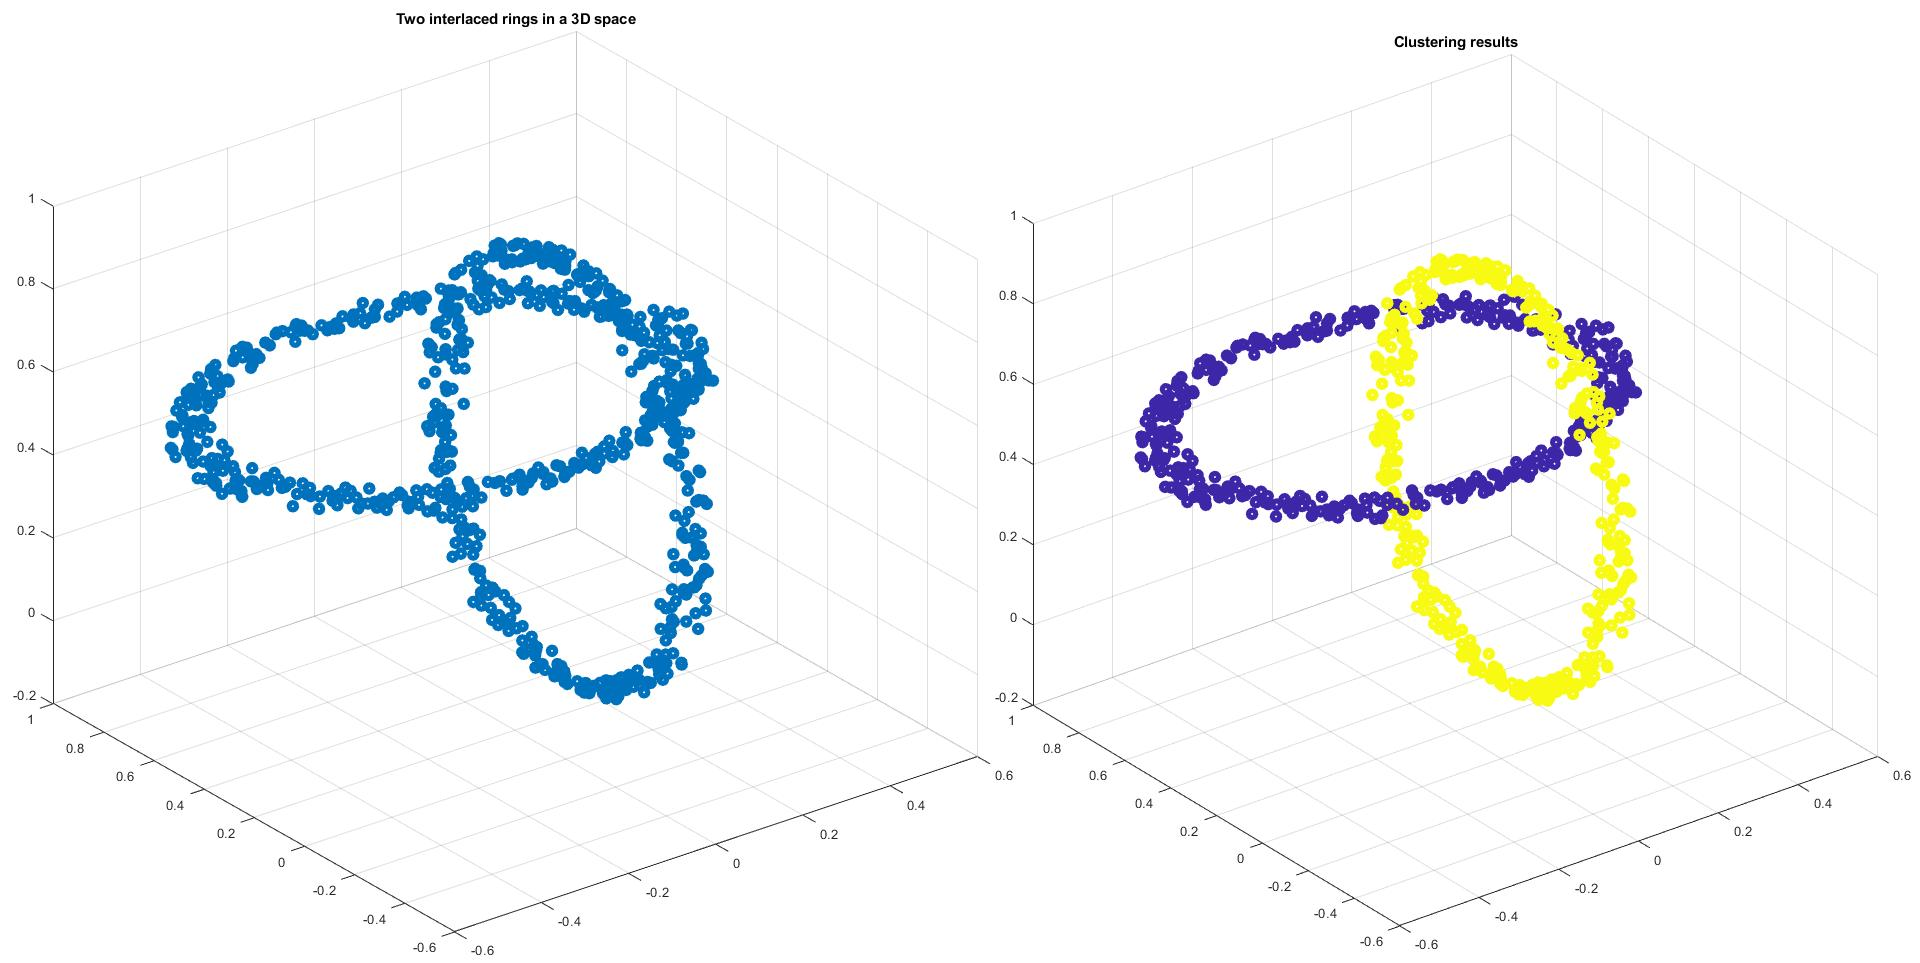
\includegraphics[height= 0.55\textwidth, width = 0.85\textwidth]{Exercise3/Report/sclust_sig_0.001.jpg}
		\caption{Clustering Results :$\sigma^2 = 0.001$ }\label{fig:sclust_sig_0.001}
	\end{subfigure}%
	\begin{subfigure}[b]{0.32\textwidth}
		\centering
		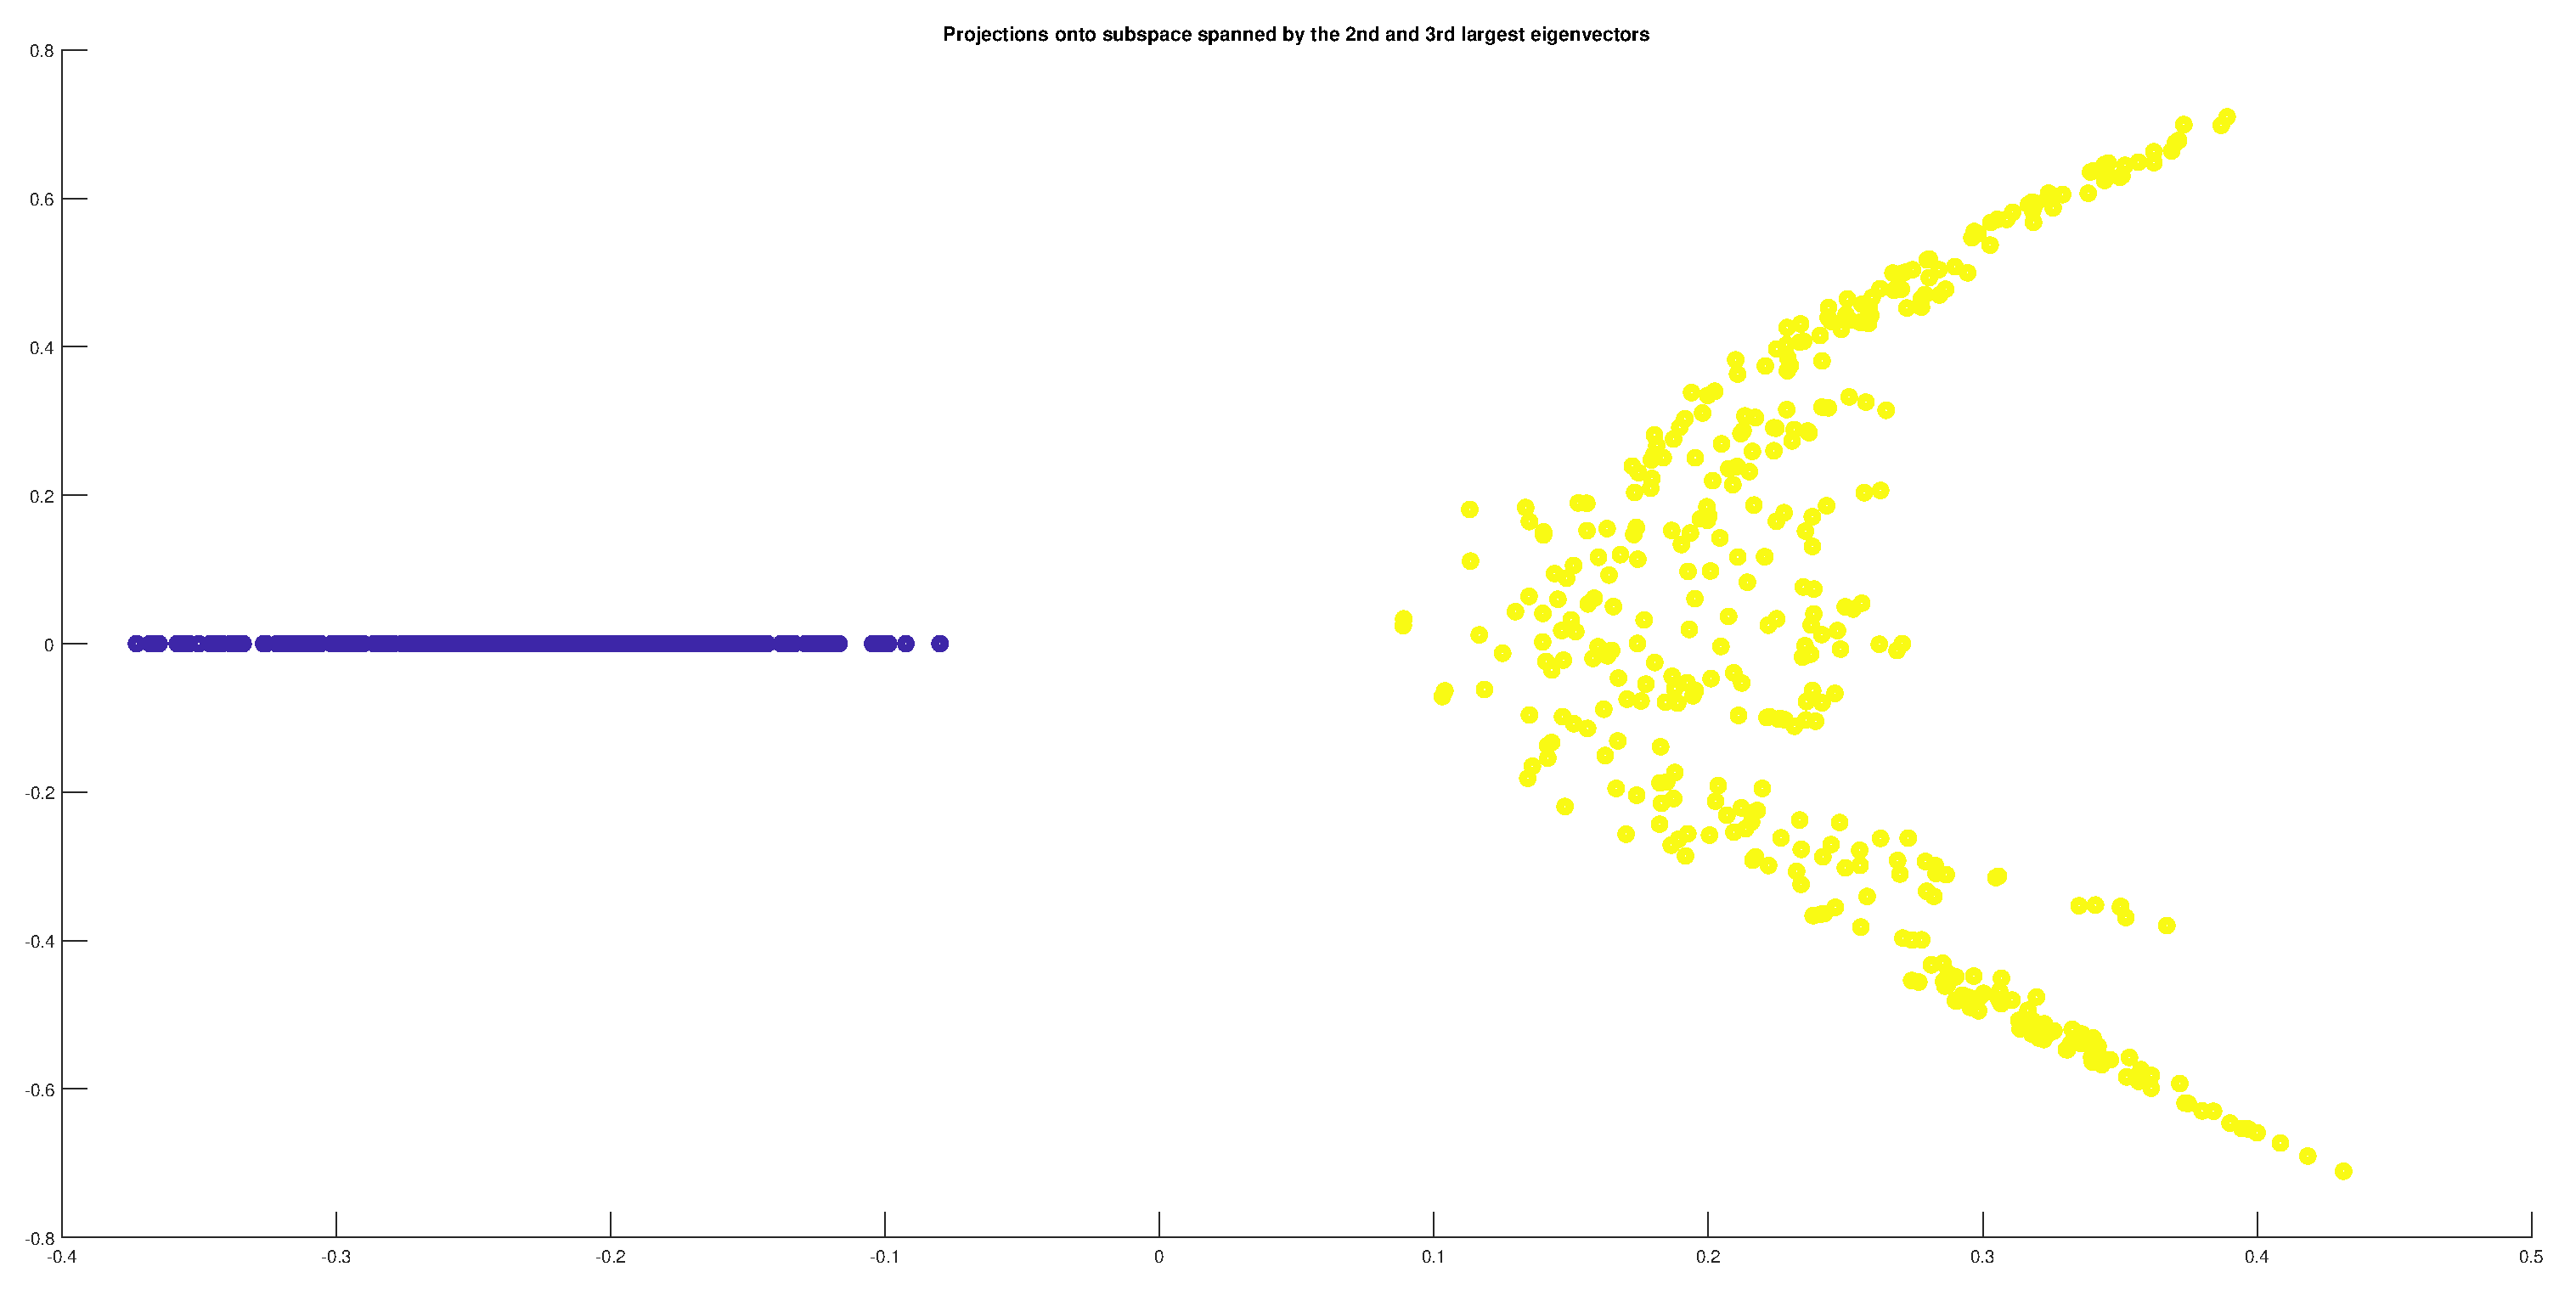
\includegraphics[height= 0.55\textwidth, width = 0.85\textwidth]{Exercise3/Report/sclust_sig_0.001_1}
		\caption{Eigen Vectors Projection}\label{fig:sclust_sig_0.001_1}
	\end{subfigure}%
	\begin{subfigure}[b]{0.32\textwidth}
		\centering
		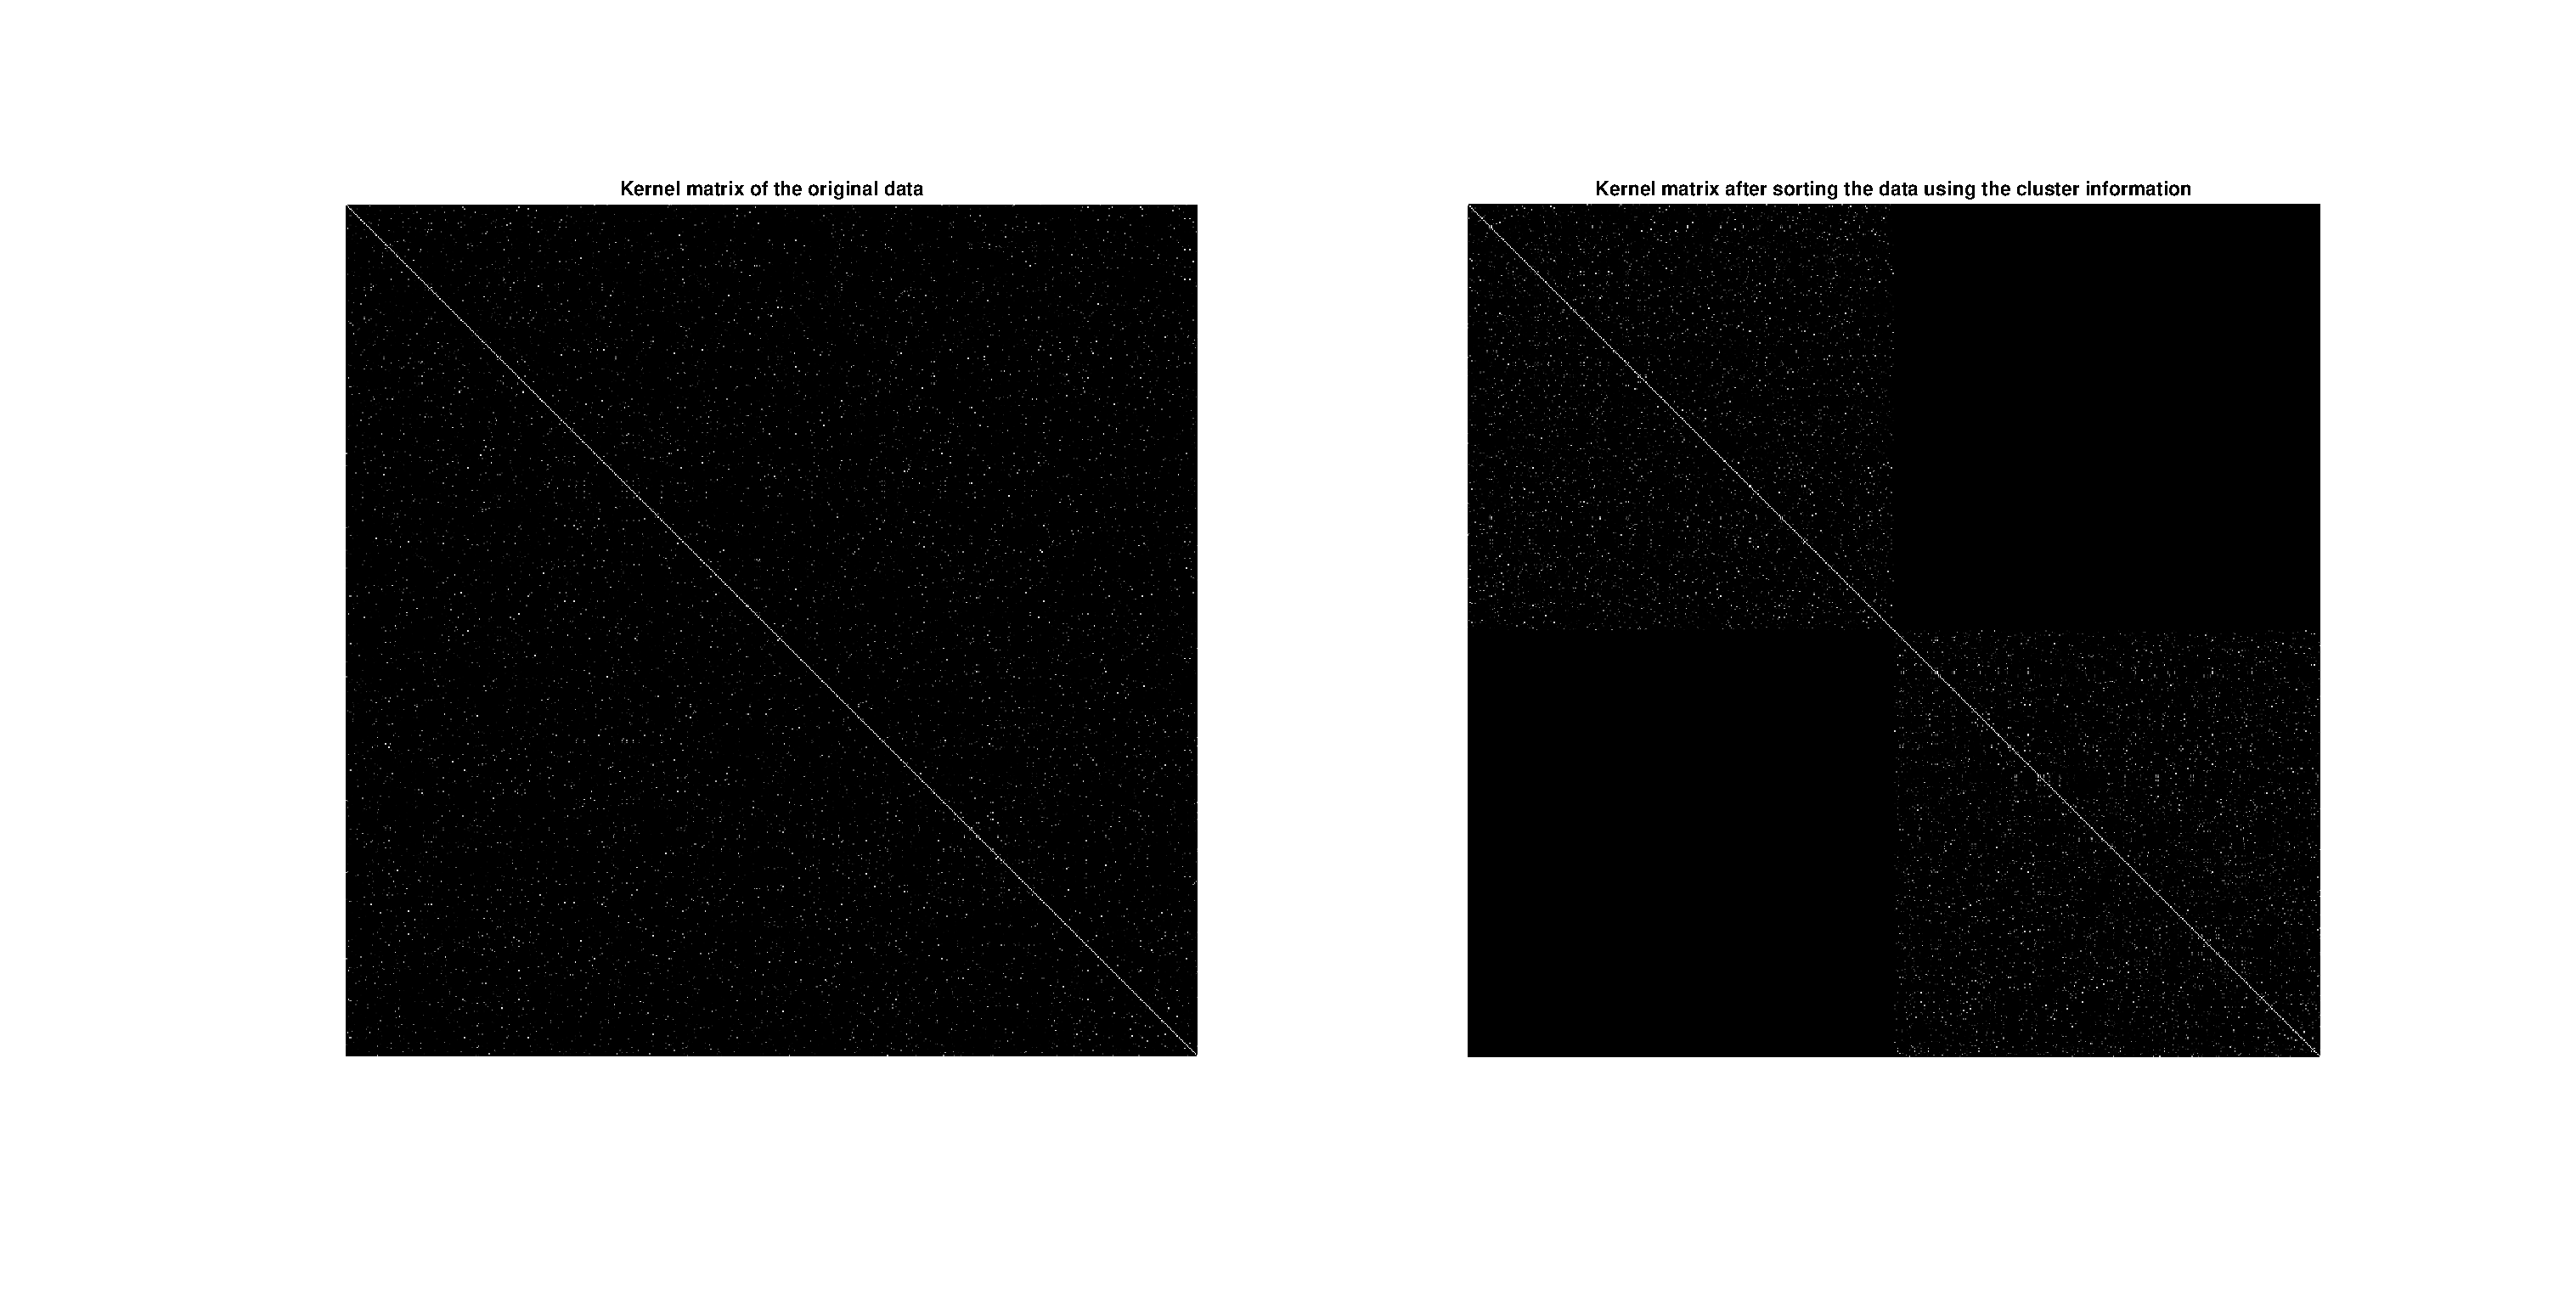
\includegraphics[height= 0.55\textwidth, width = 0.85\textwidth]{Exercise3/Report/sclust_sig_0.001_2}
		\caption{Kernel Matrix : $\sigma^2 = 0.001$}\label{fig:sclust_sig_0.001_2}
	\end{subfigure}
	\begin{subfigure}[b]{0.32\textwidth}
		\centering
		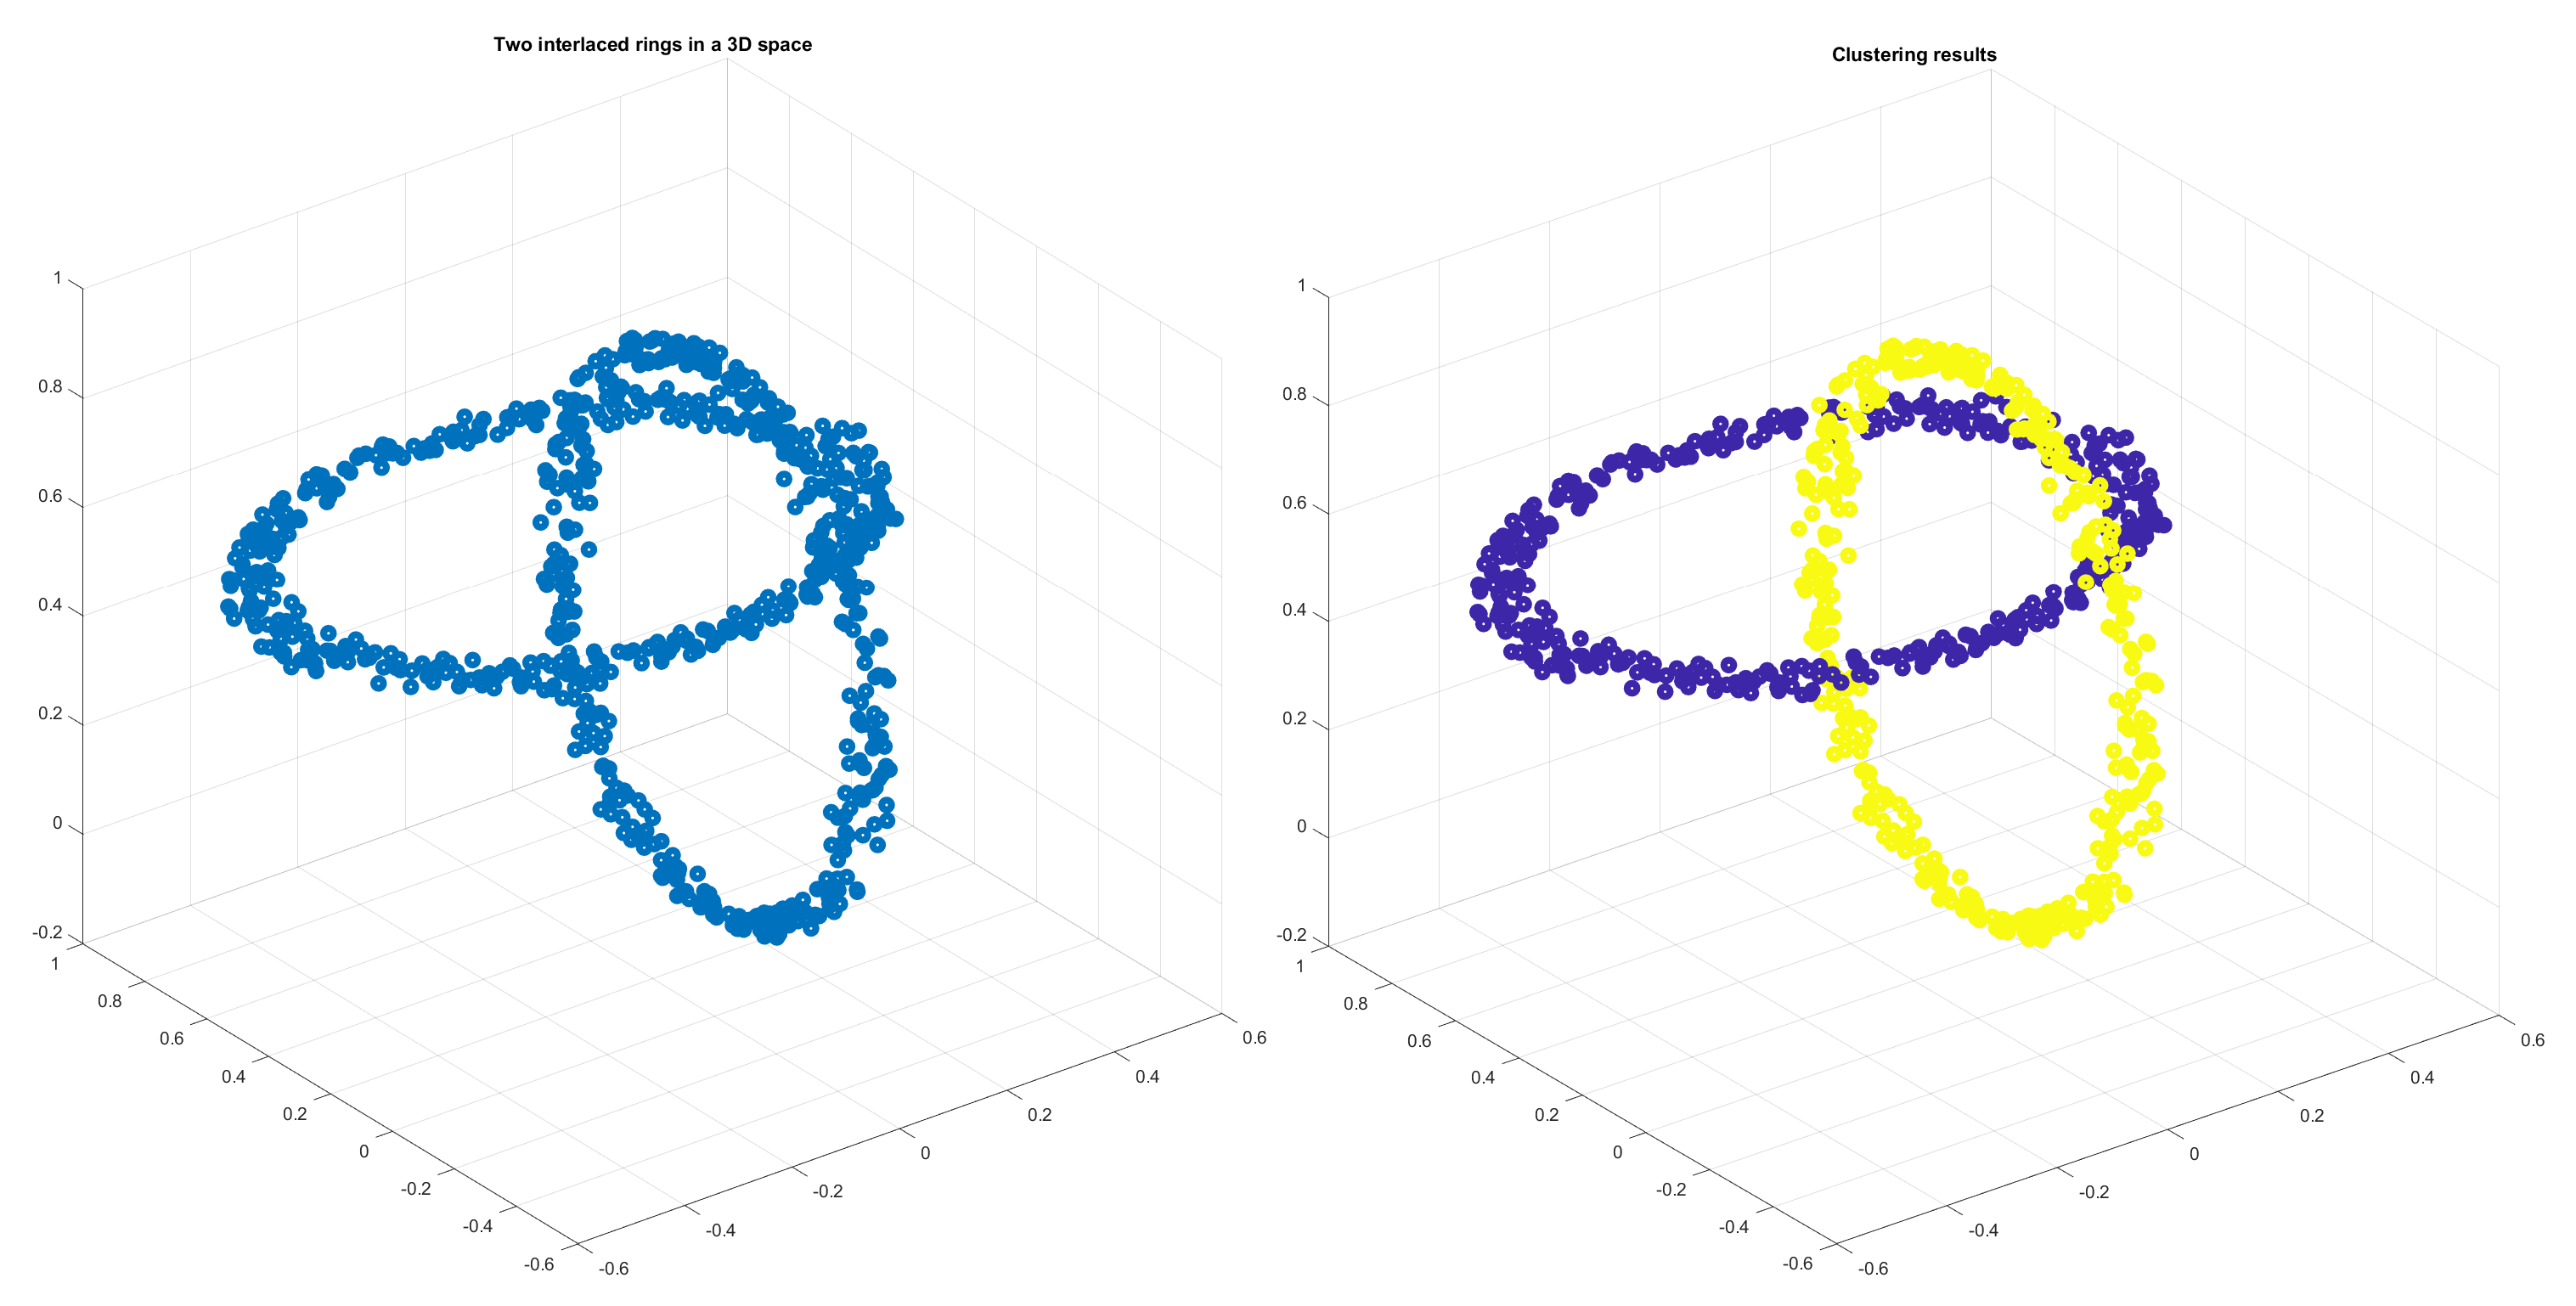
\includegraphics[height= 0.55\textwidth, width = 0.85\textwidth]{Exercise3/Report/sclust_sig_0.02.eps}
		\caption{Clustering Results : $\sigma^2 = 0.02$}\label{fig:sclust_sig_0.02}
	\end{subfigure}%
	\begin{subfigure}[b]{0.32\textwidth}
		\centering
		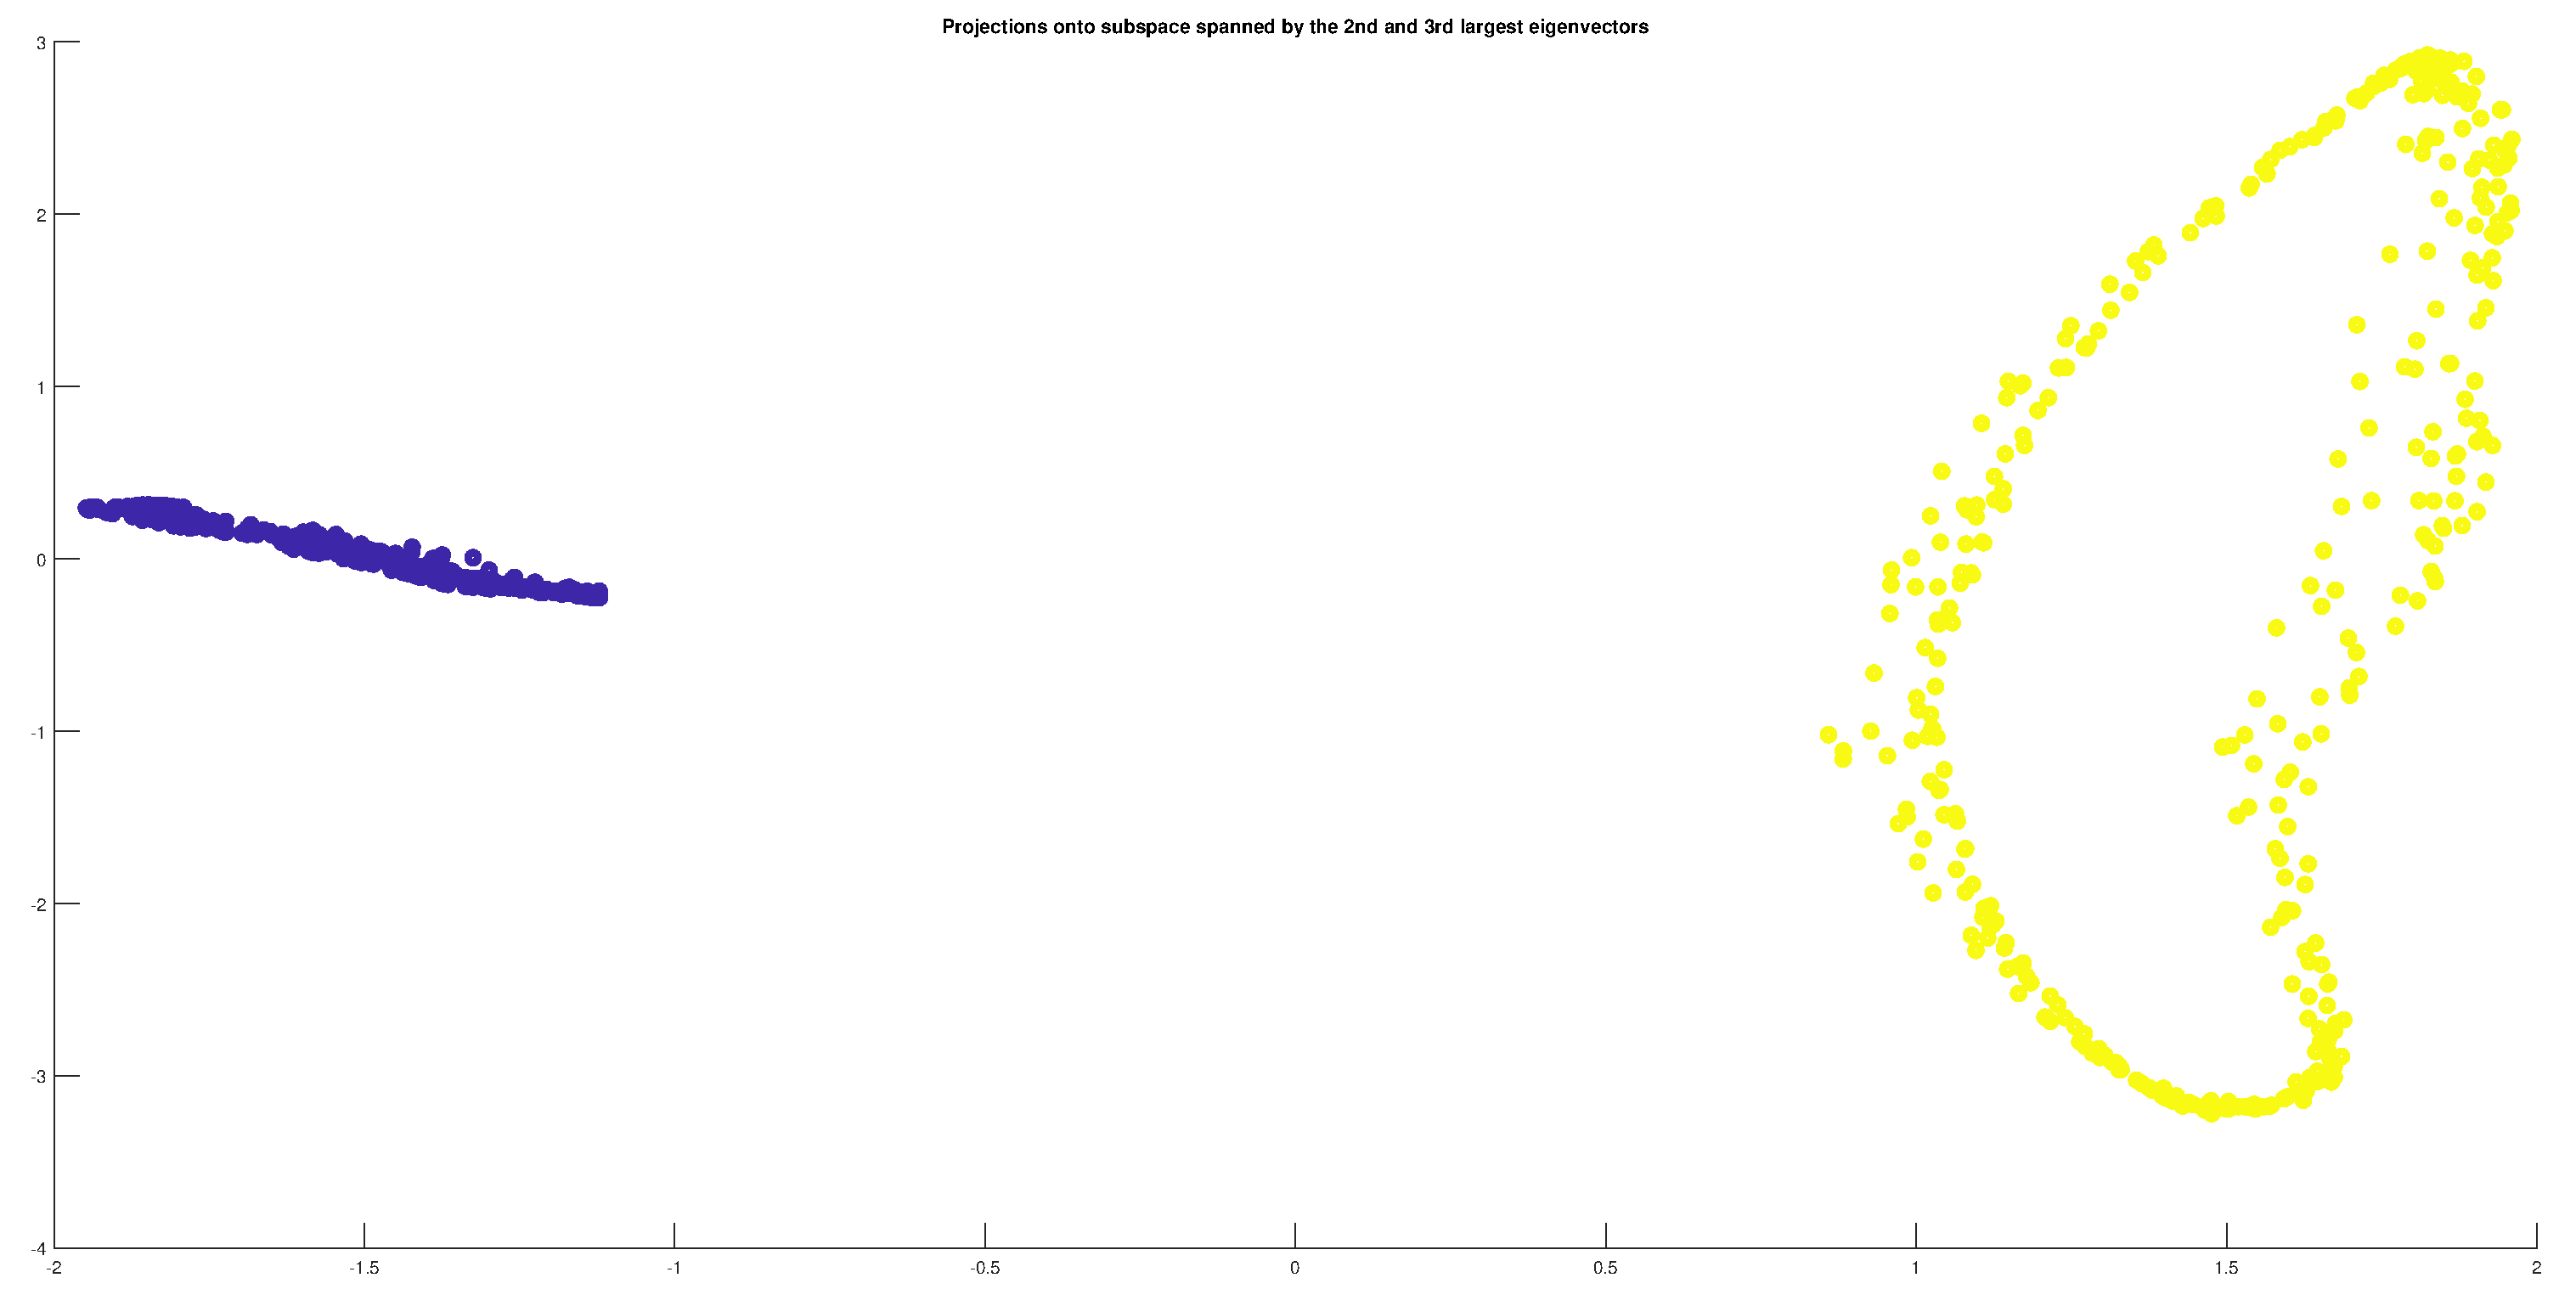
\includegraphics[height= 0.55\textwidth, width = 0.85\textwidth]{Exercise3/Report/sclust_sig_0.02_1}
		\caption{Eigen Vectors Projection }\label{fig:sclust_sig_0.02_1}
	\end{subfigure}%
	\begin{subfigure}[b]{0.32\textwidth}
		\centering
		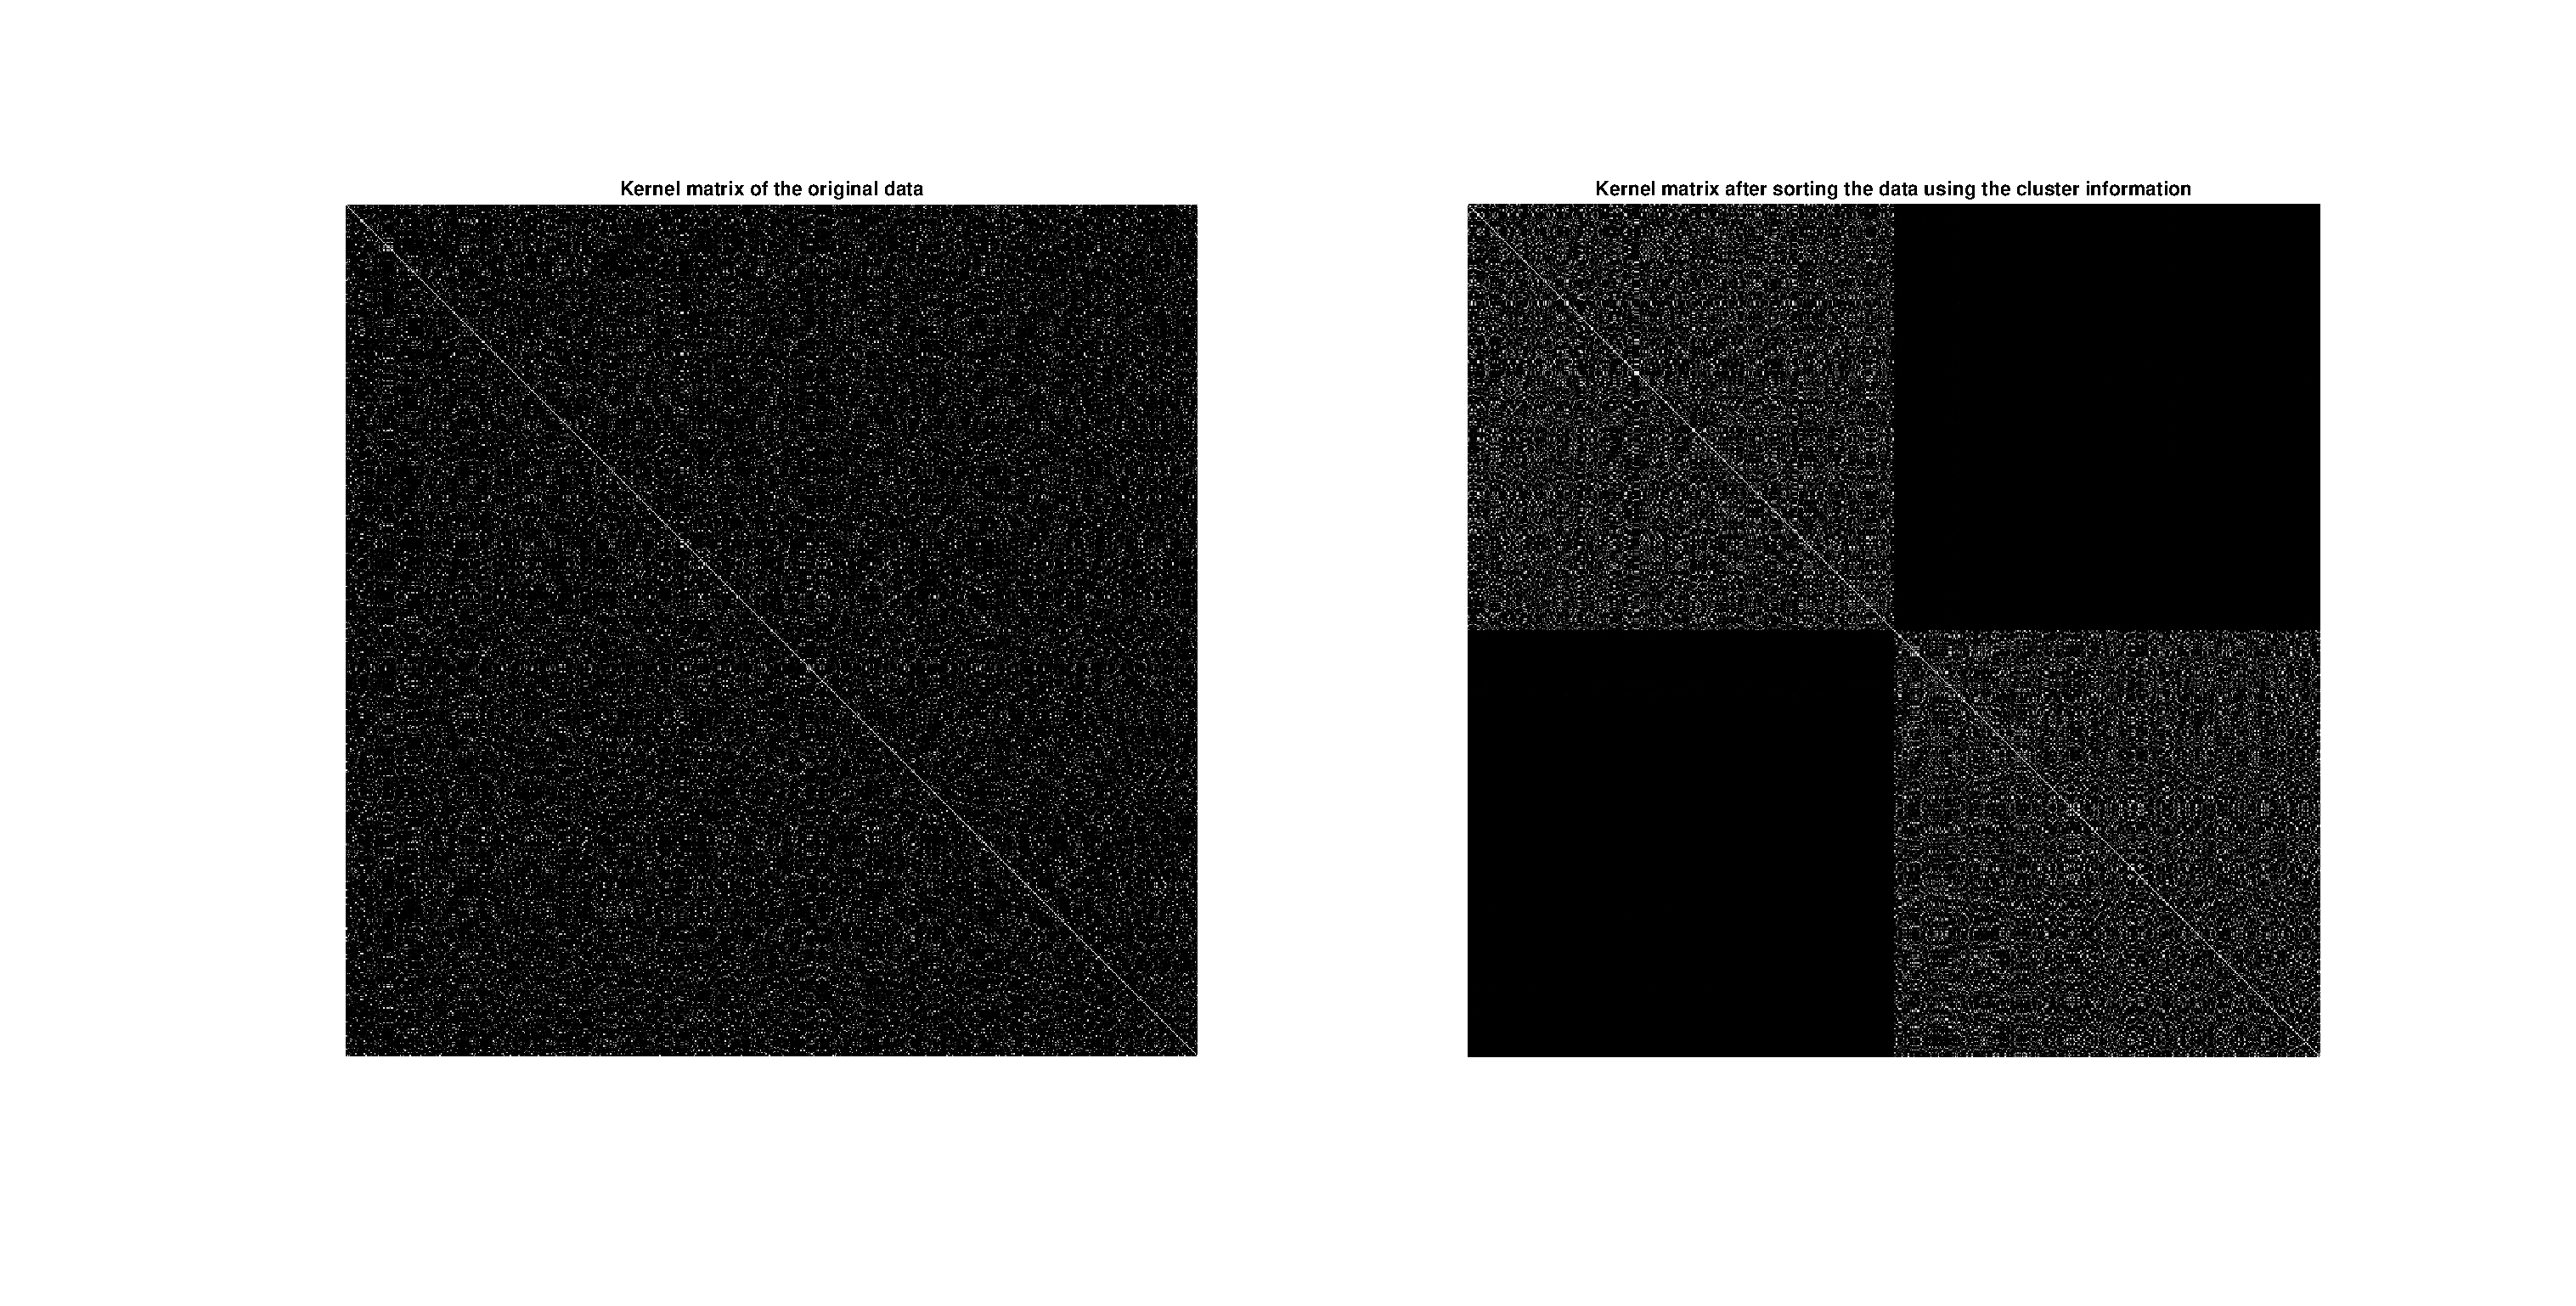
\includegraphics[height= 0.55\textwidth, width = 0.85\textwidth]{Exercise3/Report/sclust_sig_0.02_2}
		\caption{Kernel Matrix : $\sigma^2 = 0.02$}\label{fig:sclust_sig_0.02_2}
	\end{subfigure}
		\begin{subfigure}[b]{0.32\textwidth}
		\centering
		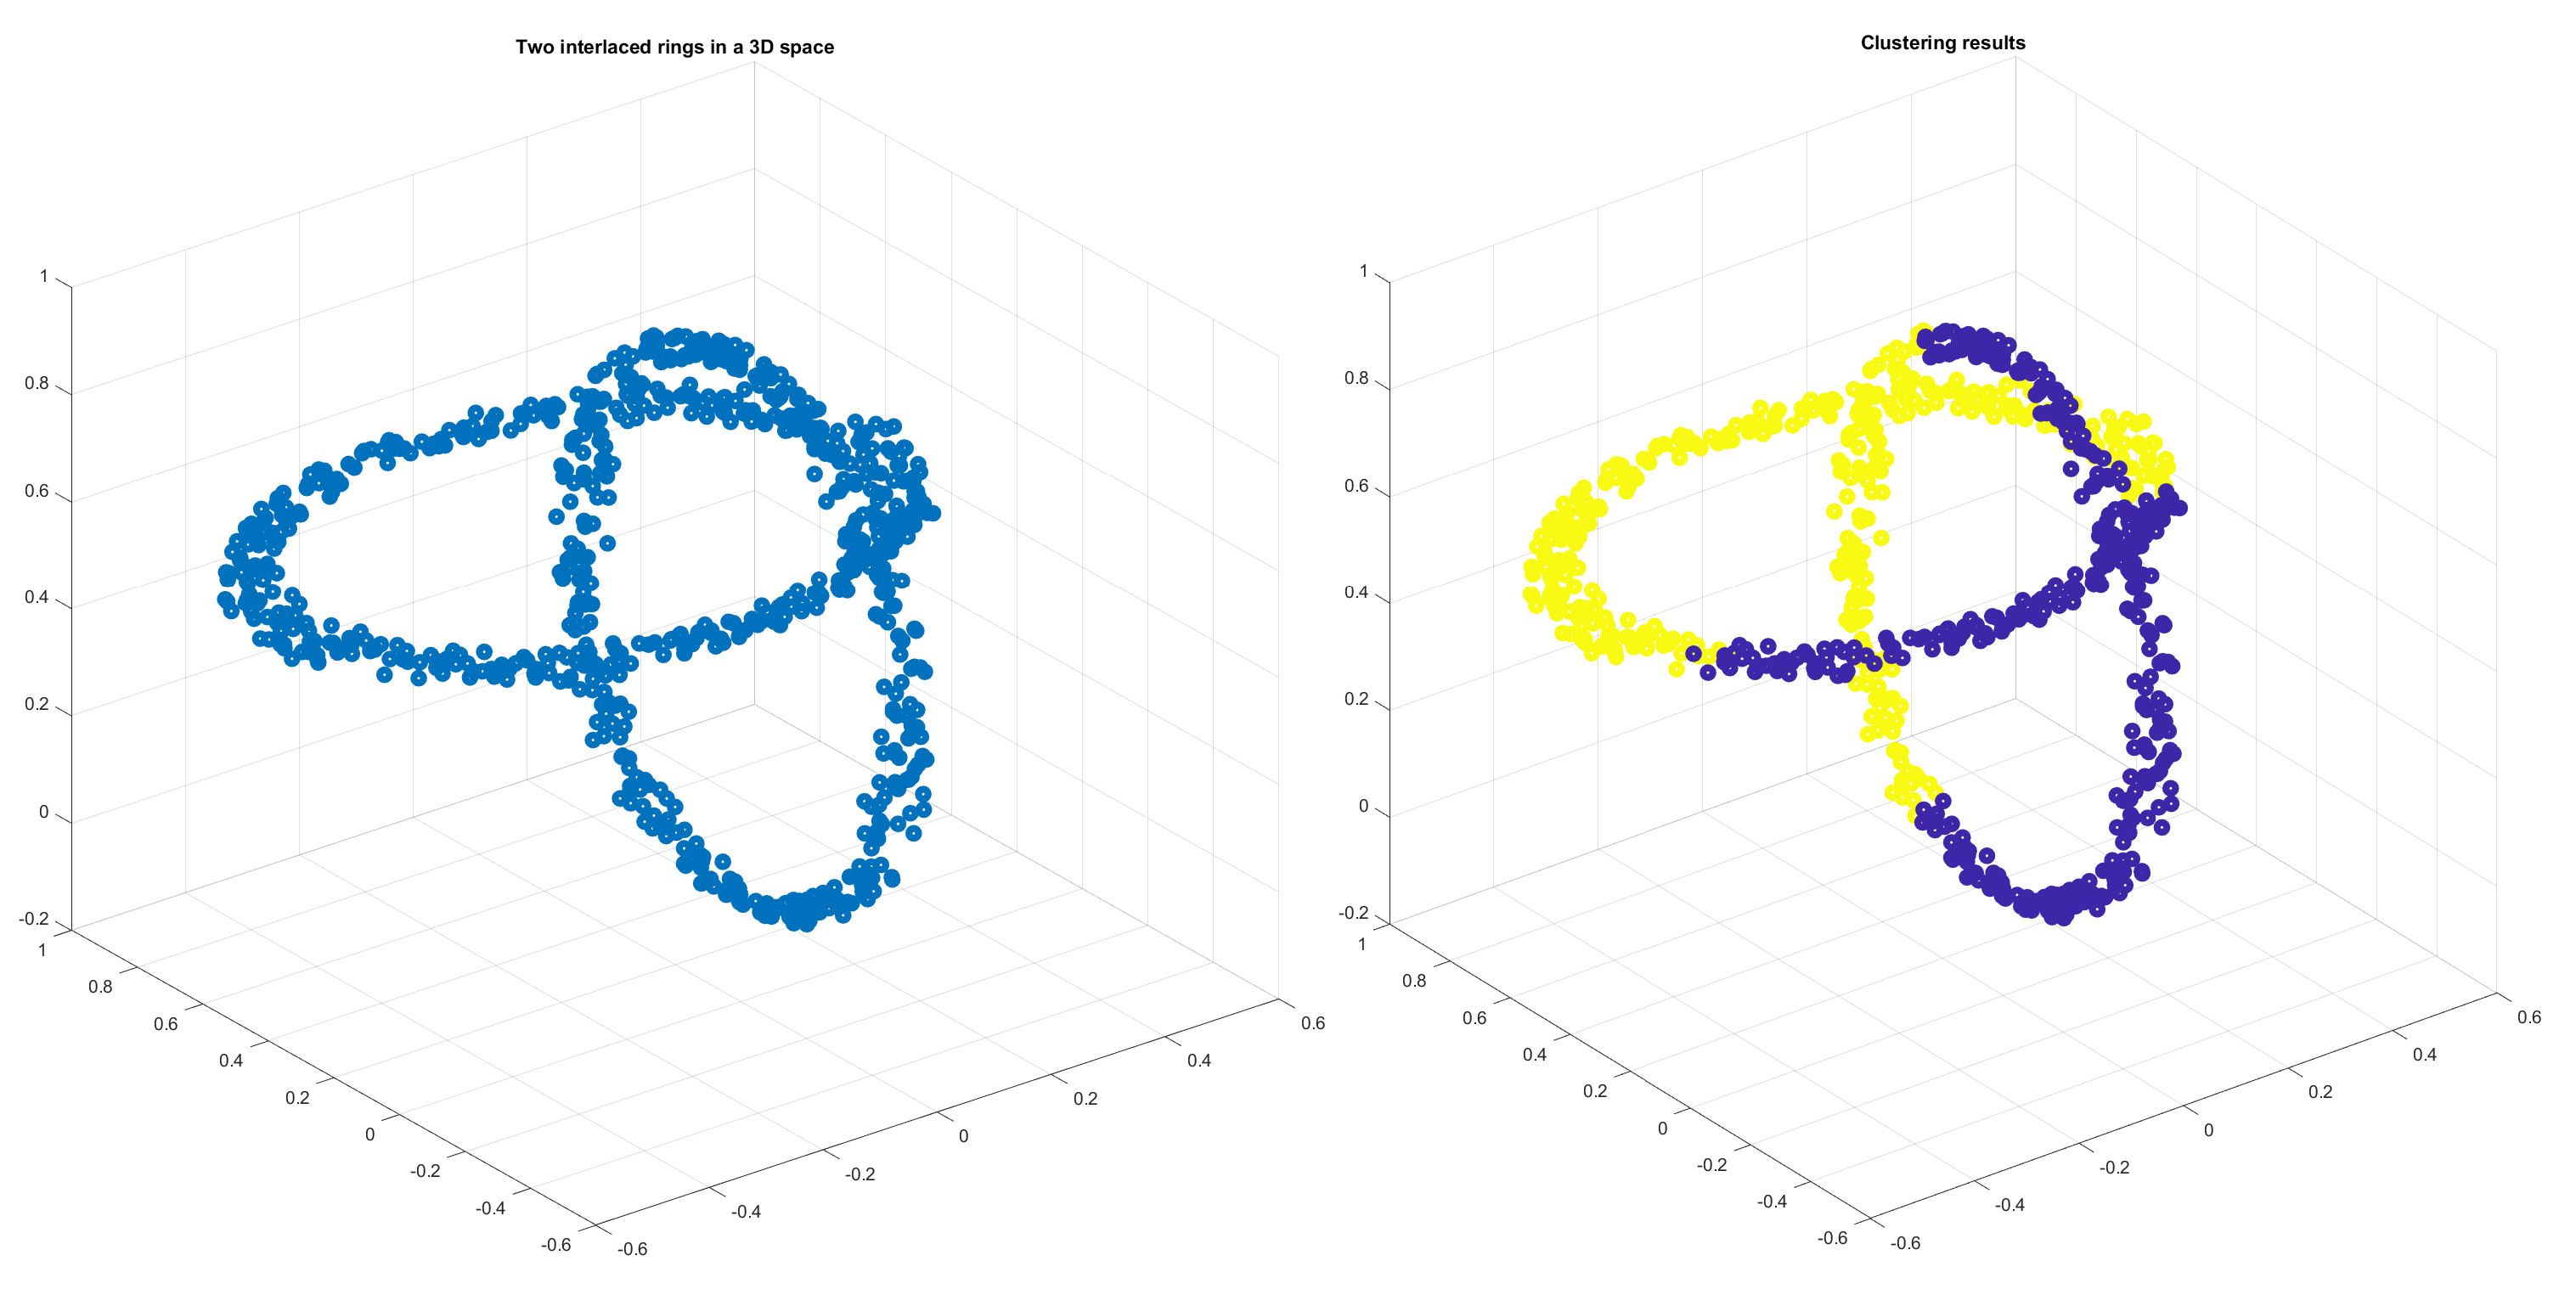
\includegraphics[height= 0.55\textwidth, width = 0.85\textwidth]{Exercise3/Report/sclust_sig_1.eps}
		\caption{Clustering Results : $\sigma^2 = 1$ }\label{fig:sclust_sig_1}
	\end{subfigure}%
	\begin{subfigure}[b]{0.32\textwidth}
		\centering
		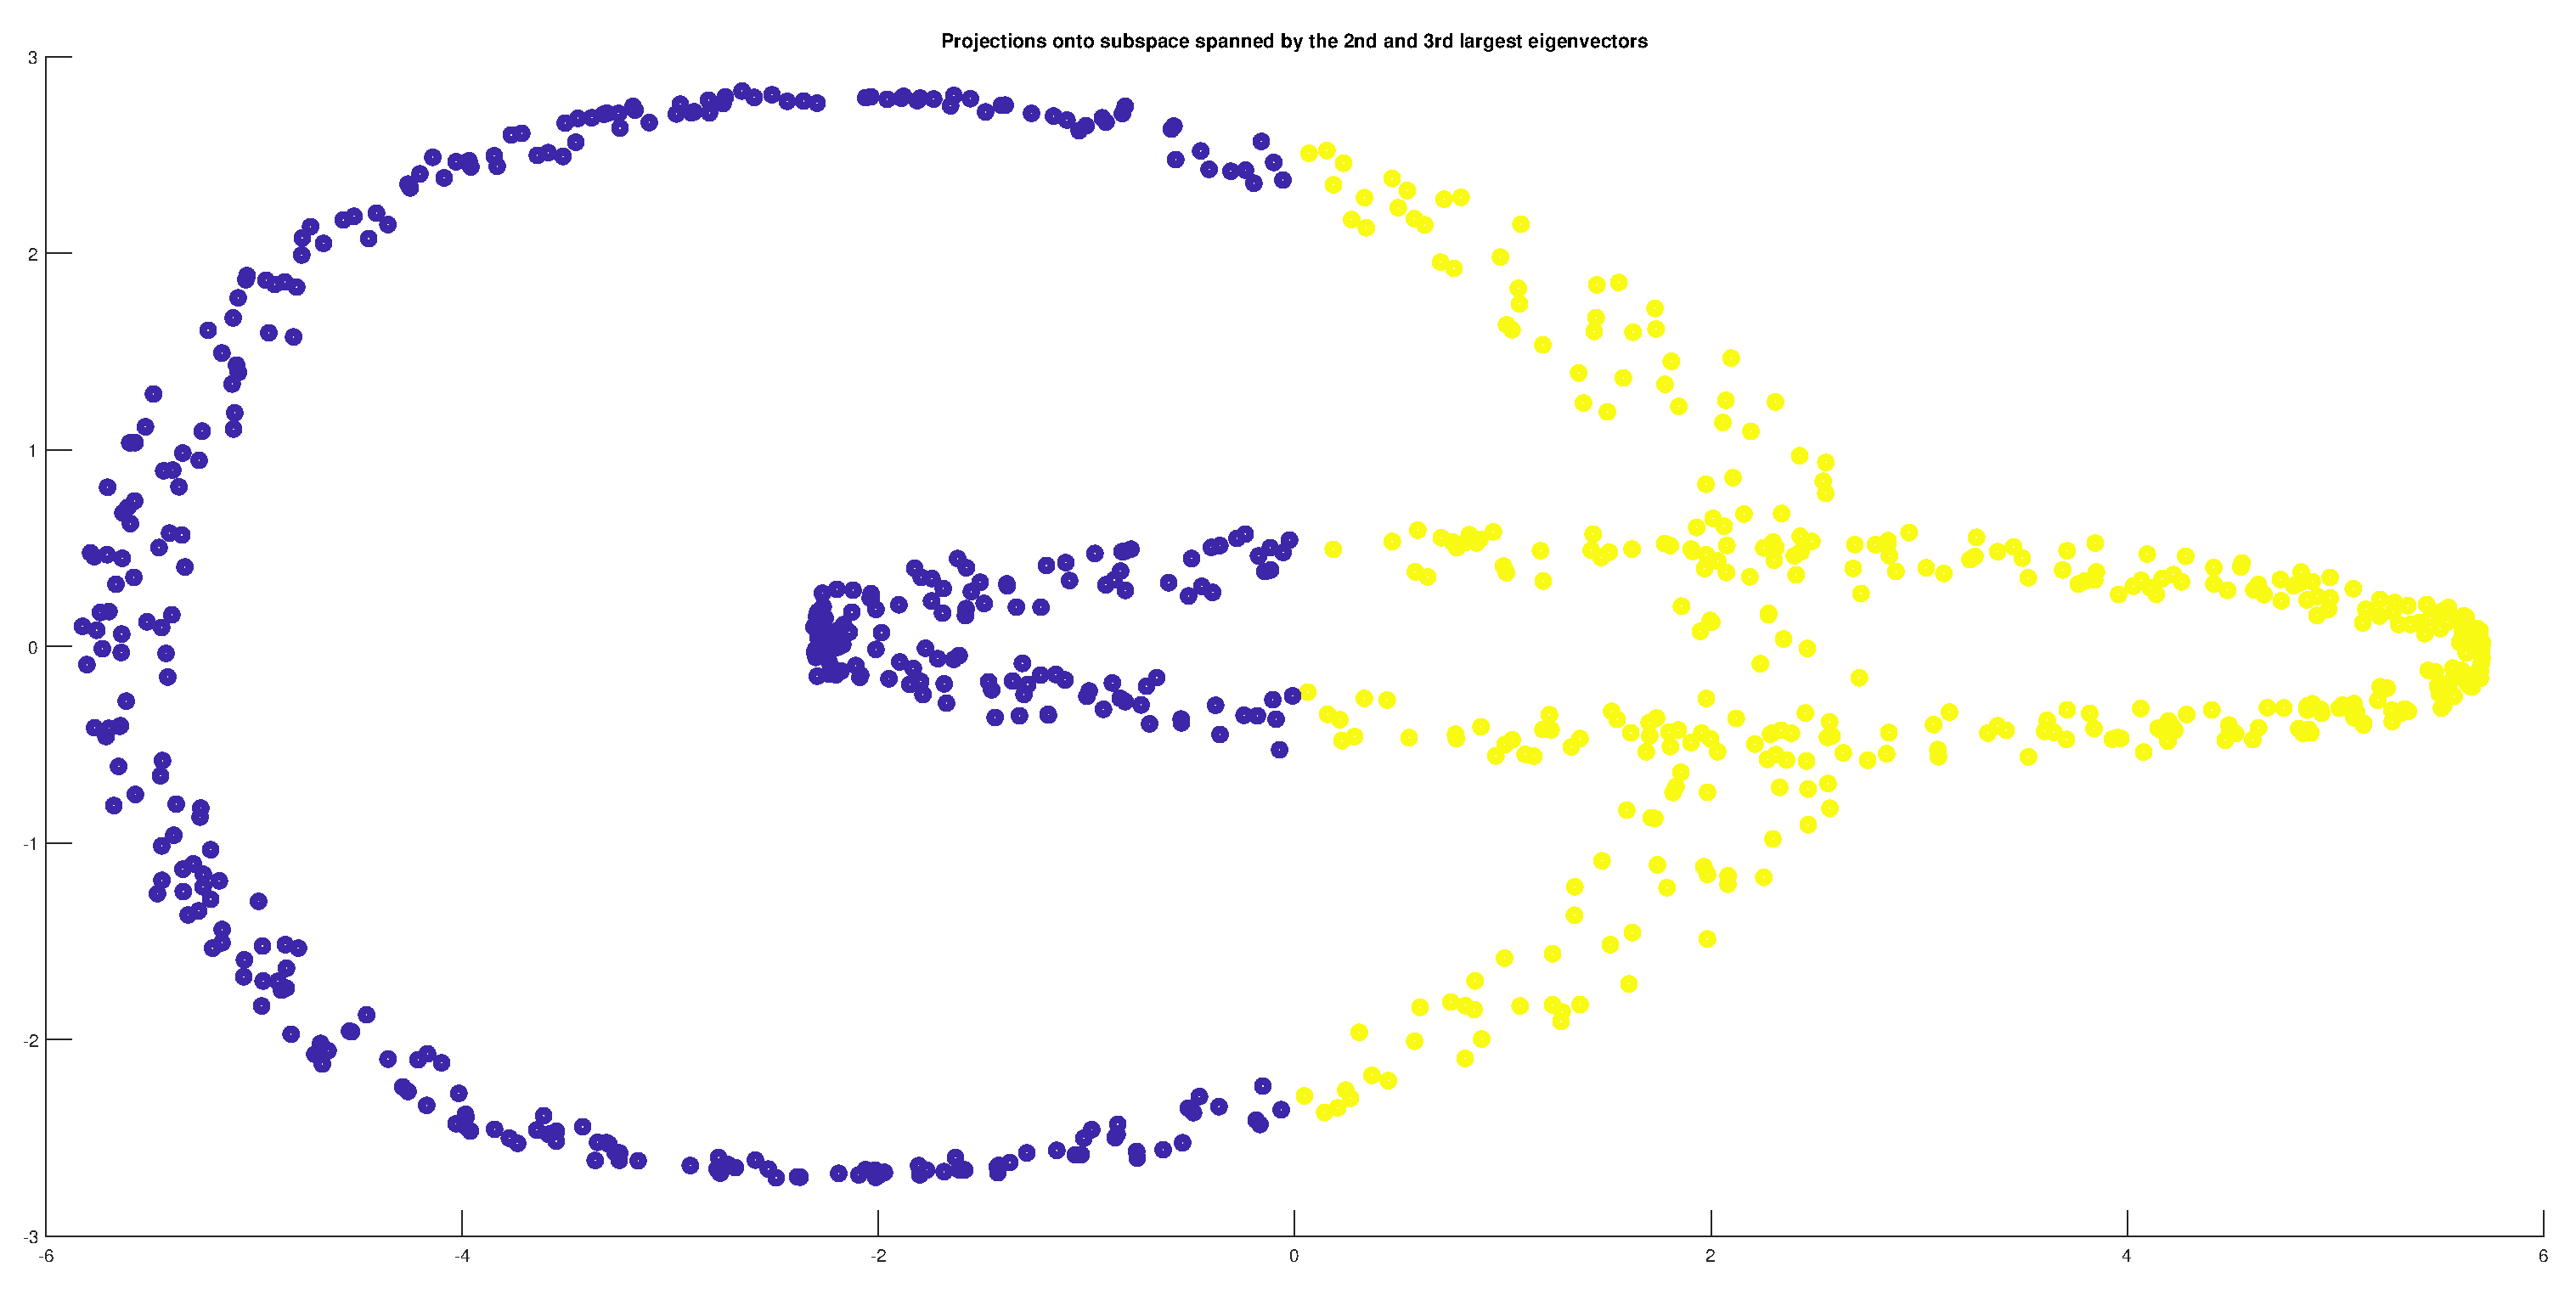
\includegraphics[height= 0.55\textwidth, width = 0.85\textwidth]{Exercise3/Report/sclust_sig_1_1}
		\caption{Eigen Vectors Projection}\label{fig:sclust_sig_1_1}
	\end{subfigure}%
	\begin{subfigure}[b]{0.32\textwidth}
		\centering
		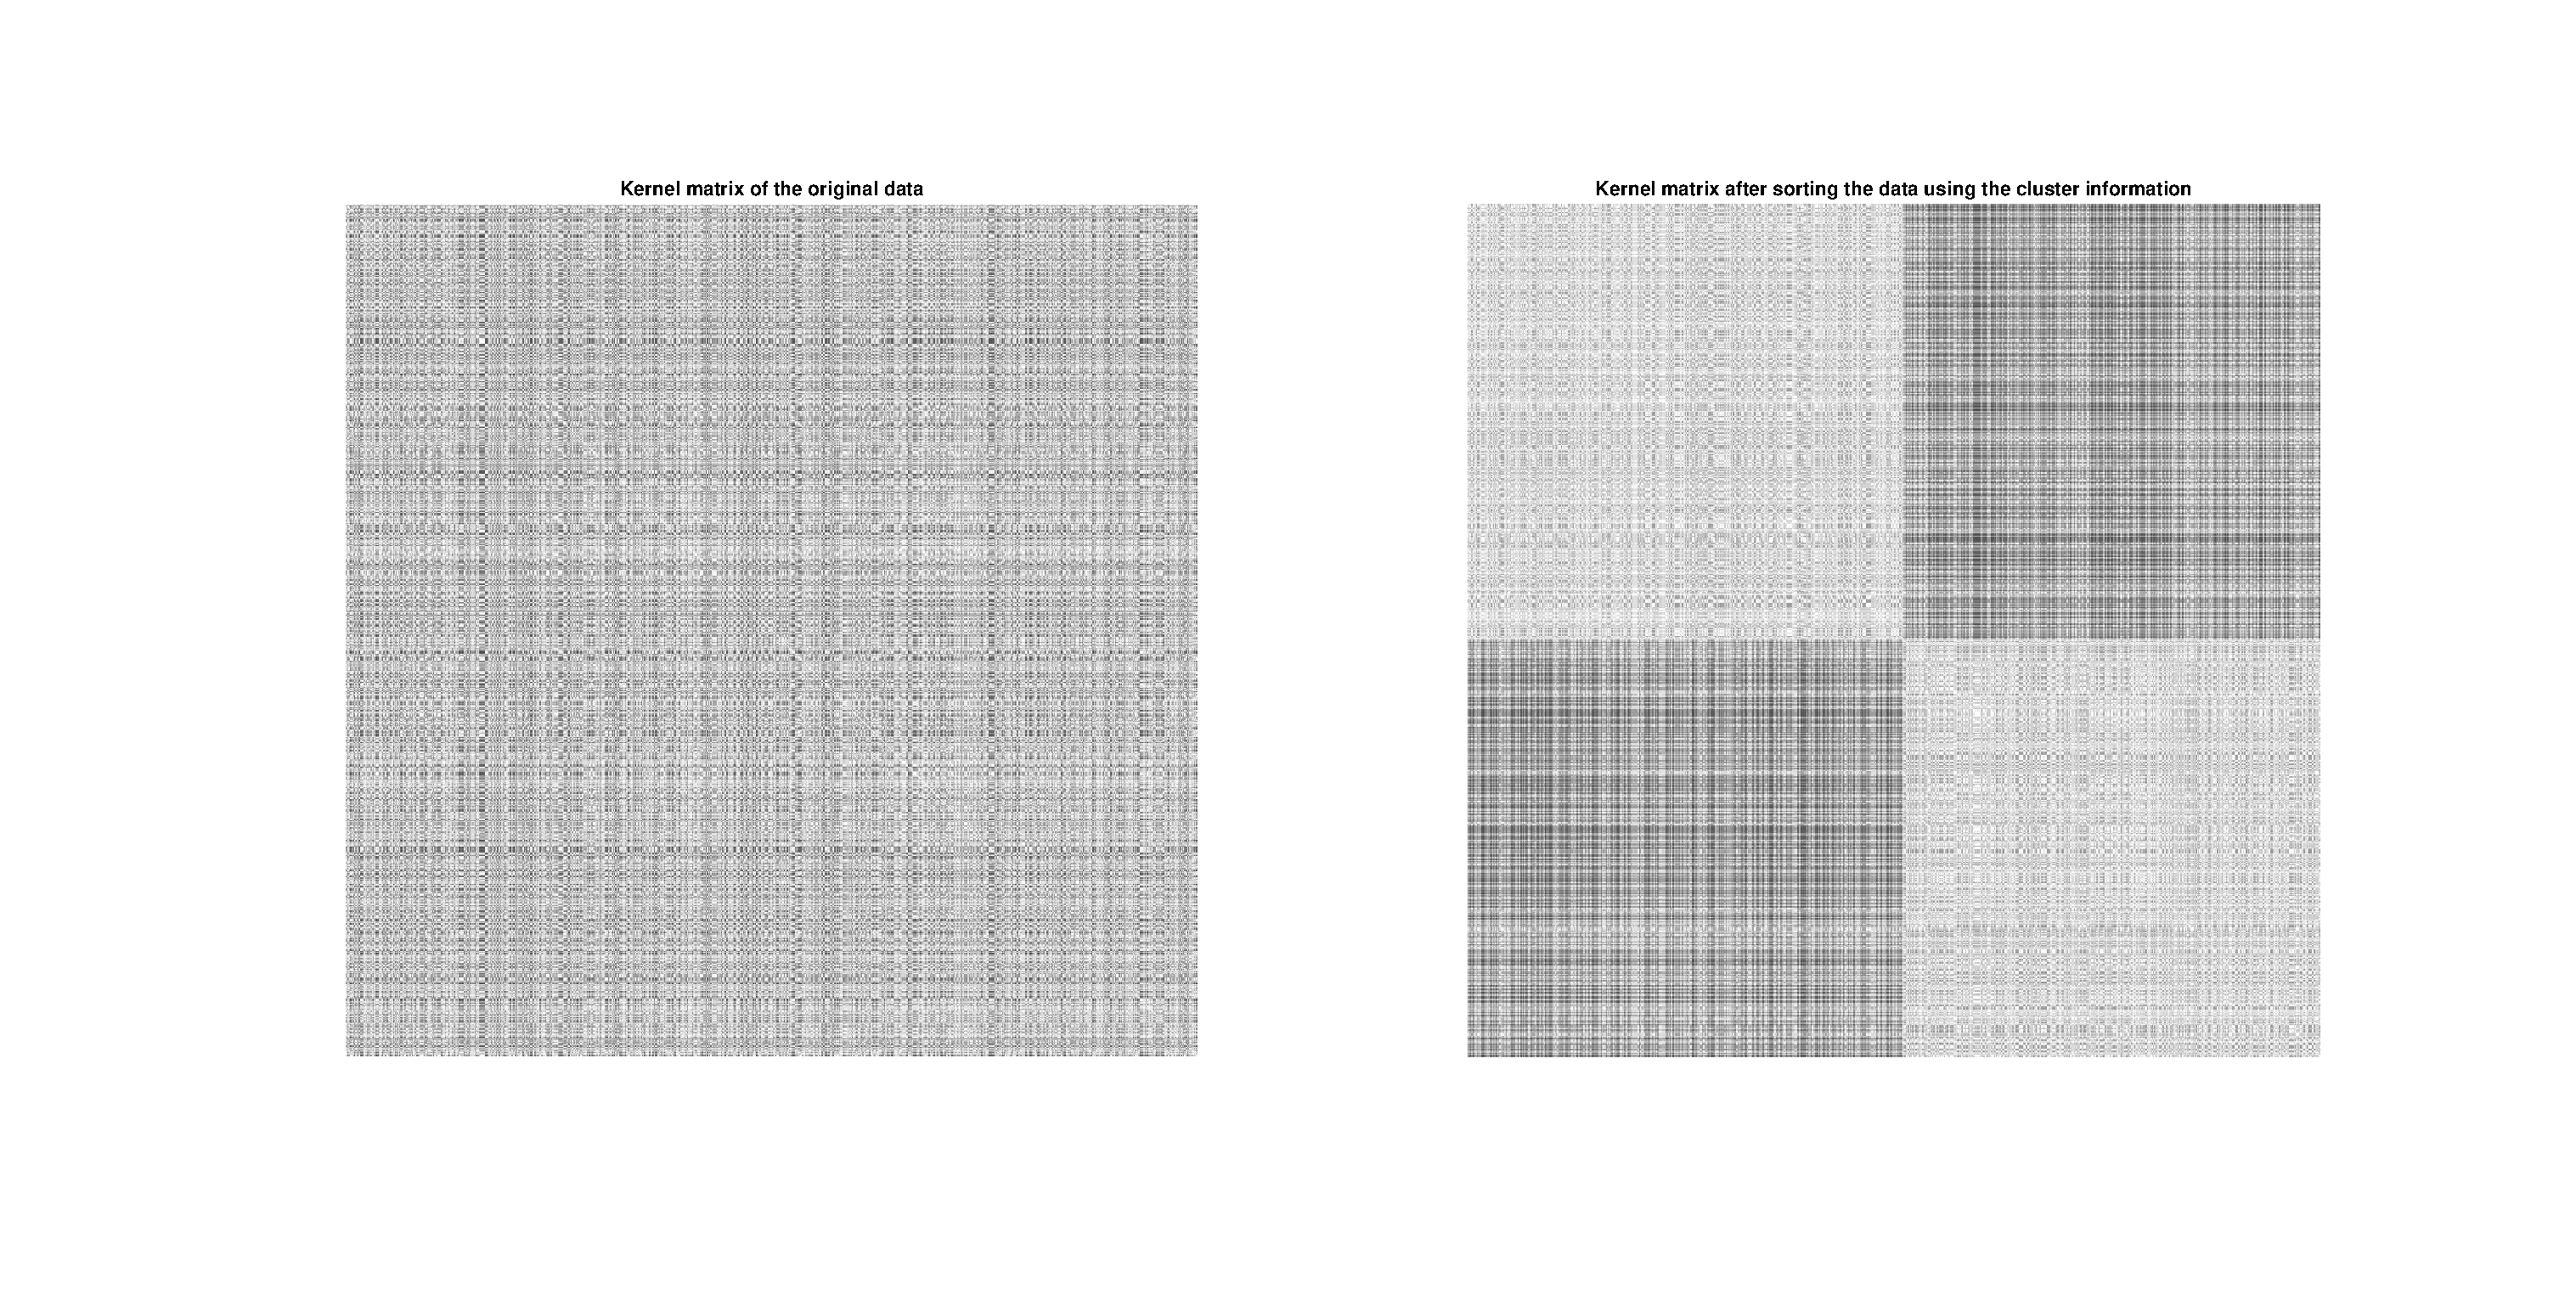
\includegraphics[height= 0.55\textwidth, width = 0.85\textwidth]{Exercise3/Report/sclust_sig_1_2}
		\caption{Kernel Matrix : $\sigma^2 = 1$}\label{fig:sclust_sig_1_2}
	\end{subfigure}
	\caption{Spectral Clustering Results; ($\sigma^2$) = (0.001;0.02;1) }
	\label{fig:sclust}
\end{figure}\\
\subsection{Fixed-size LS-SVM}
Solving a model in primal space would be useful for large datasets whereas dual space would be suitable for large dimensional inputs. \\\\ 
\textbf{What is the effect of the chosen kernel parameter sig2 on the resulting fixed-size subset of data points (see fixedsize script1.m)? Can you intuitively describe to what subset the algorithm converges?}

The function \textit{kentropy} uses Quadratic Renyi Entropy in the selection of the subset. The algorithm selects the subset when it converges to the subset with maximum entropy and the subset gives a better representation of the original data. The algorithm is run with 6 different hyper parameters of $\sigma^2$ (0.001 ; 0.01 ; 0.1 ; 1 ; 10 ; 100). Some of the results are plotted in the figure \ref{fig:fixedlssvm}. For lower values of $\sigma^2$, the chosen support vectors are very close and as the $\sigma^2$ increases, the support vectors spread out evenly  away from the data point. From the figure \ref{fig:fixed_lssvm_sig_100}, it can be seen that all the support vectors are mostly outliers. For $\sigma^2$ = 0.1 and 1, the chosen candidates have better entropy and a gives a good representation of the data set.
\begin{figure}[!htpb]
	\begin{subfigure}[b]{0.25\textwidth}
		\centering
		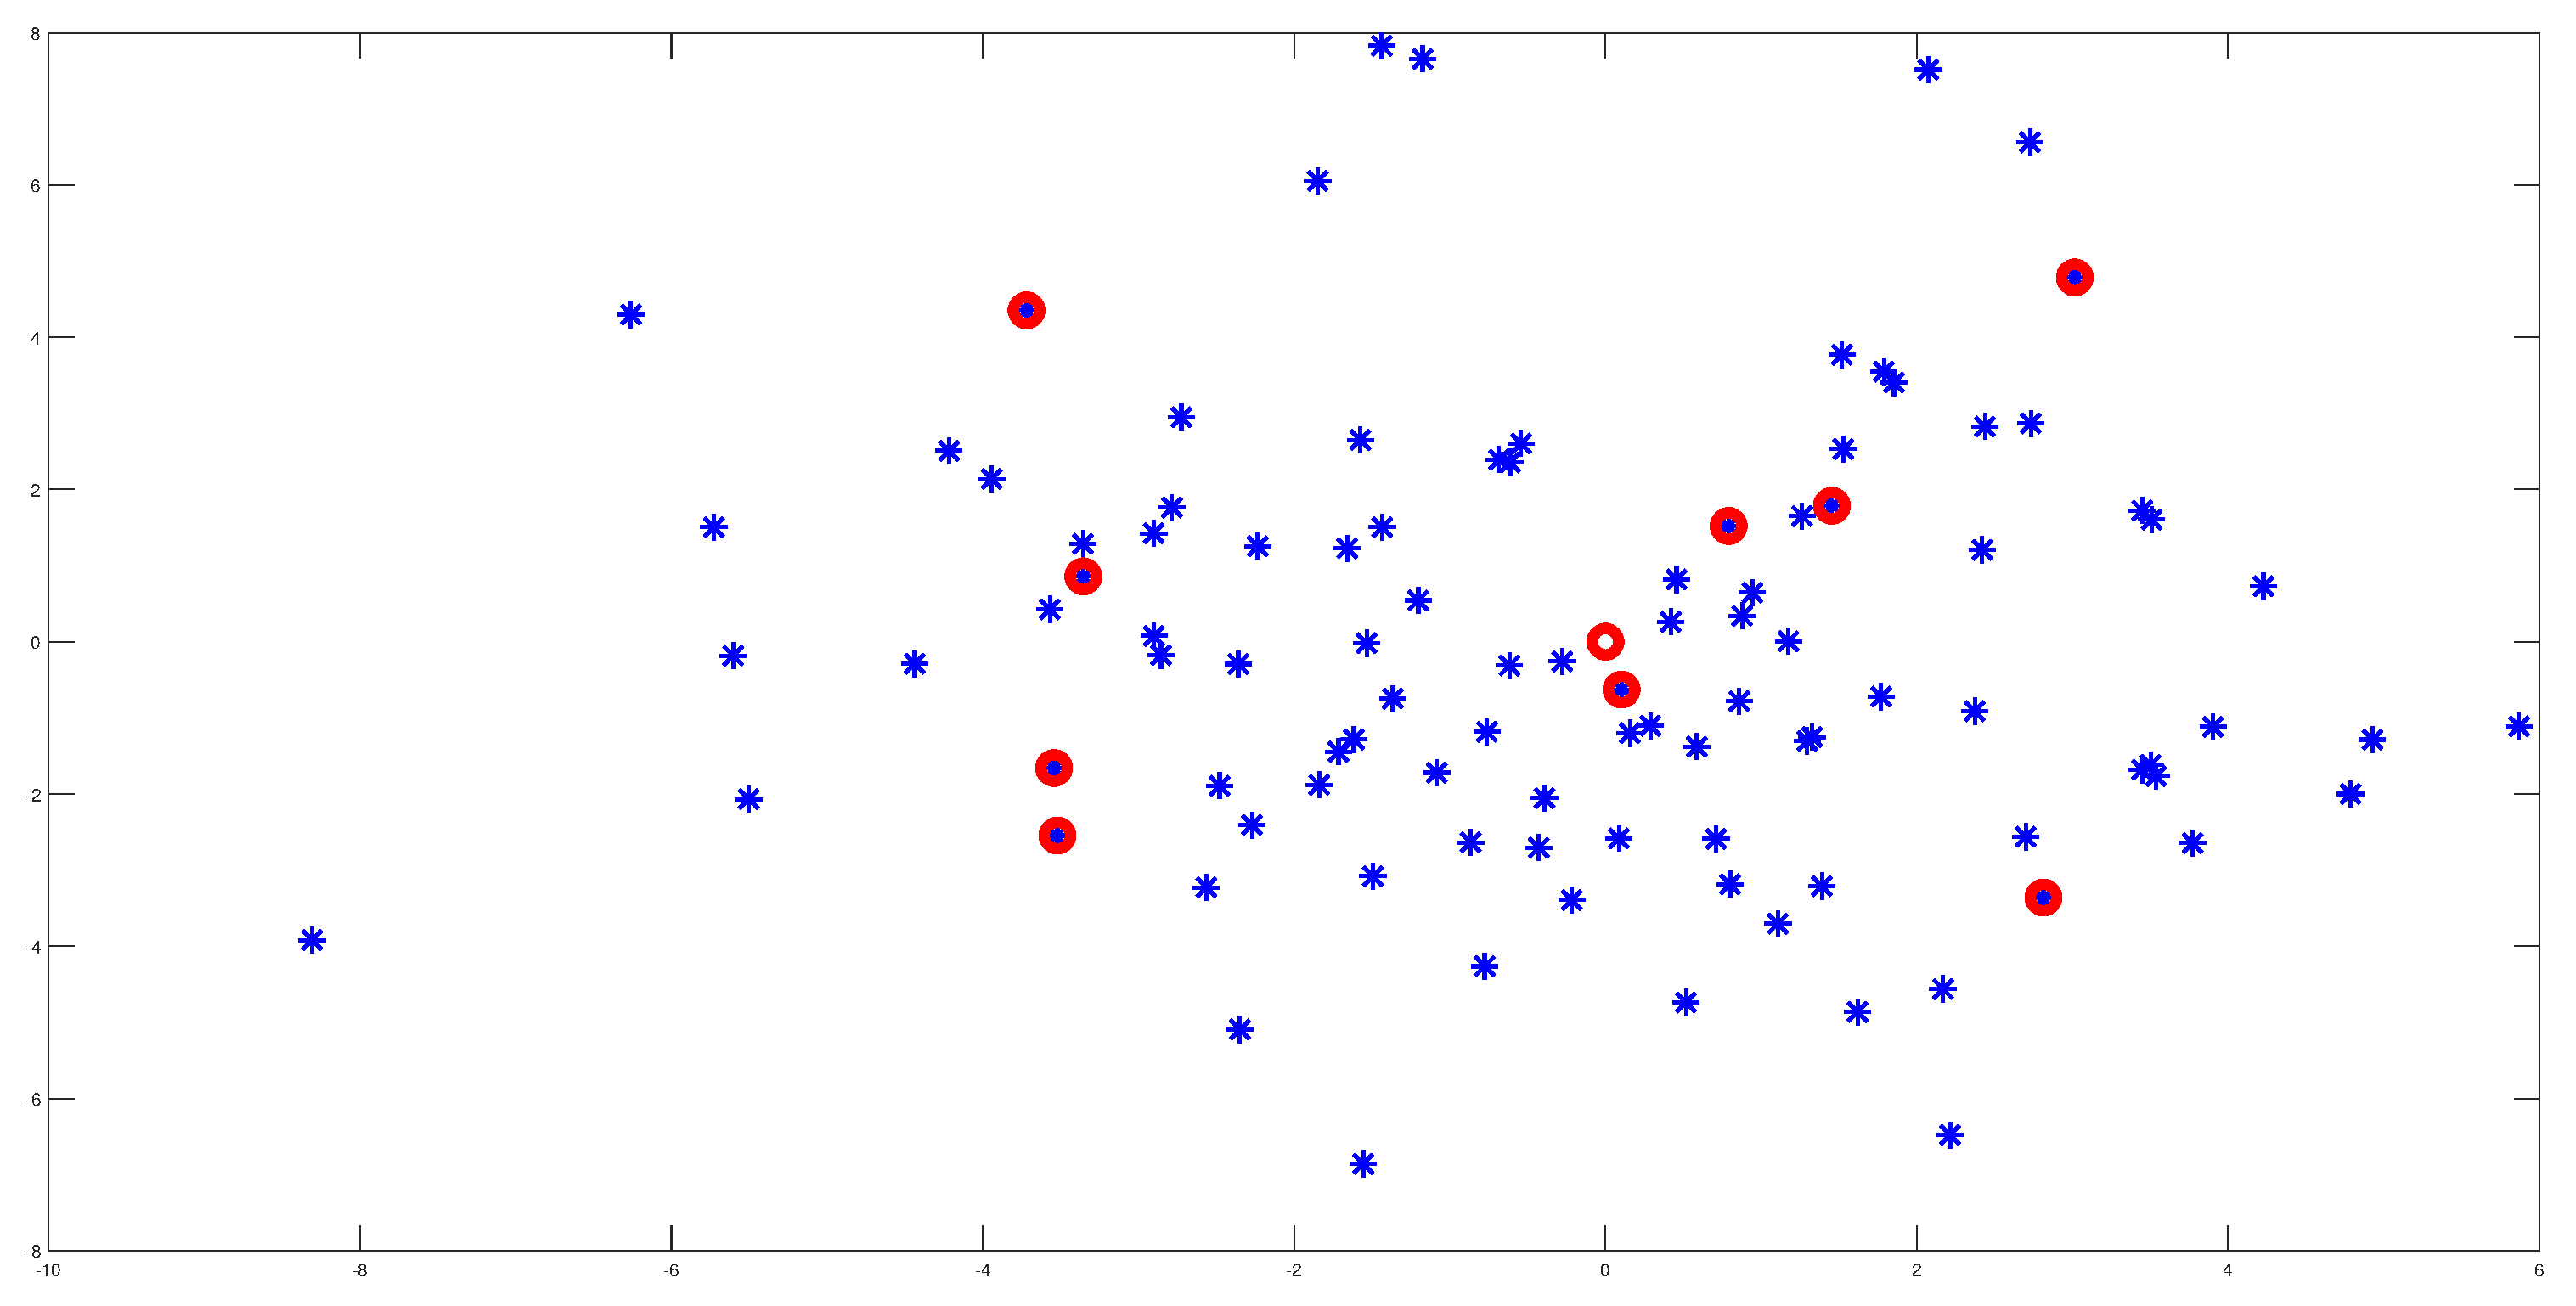
\includegraphics[height= 0.65\textwidth, width = 0.9\textwidth]{Exercise3/Report/fixed_lssvm_sig_0.001}
		\caption{$\sigma^2 = 0.001$ }\label{fig:fixed_lssvm_sig_0.001}
	\end{subfigure}%
	\begin{subfigure}[b]{0.25\textwidth}
		\centering
		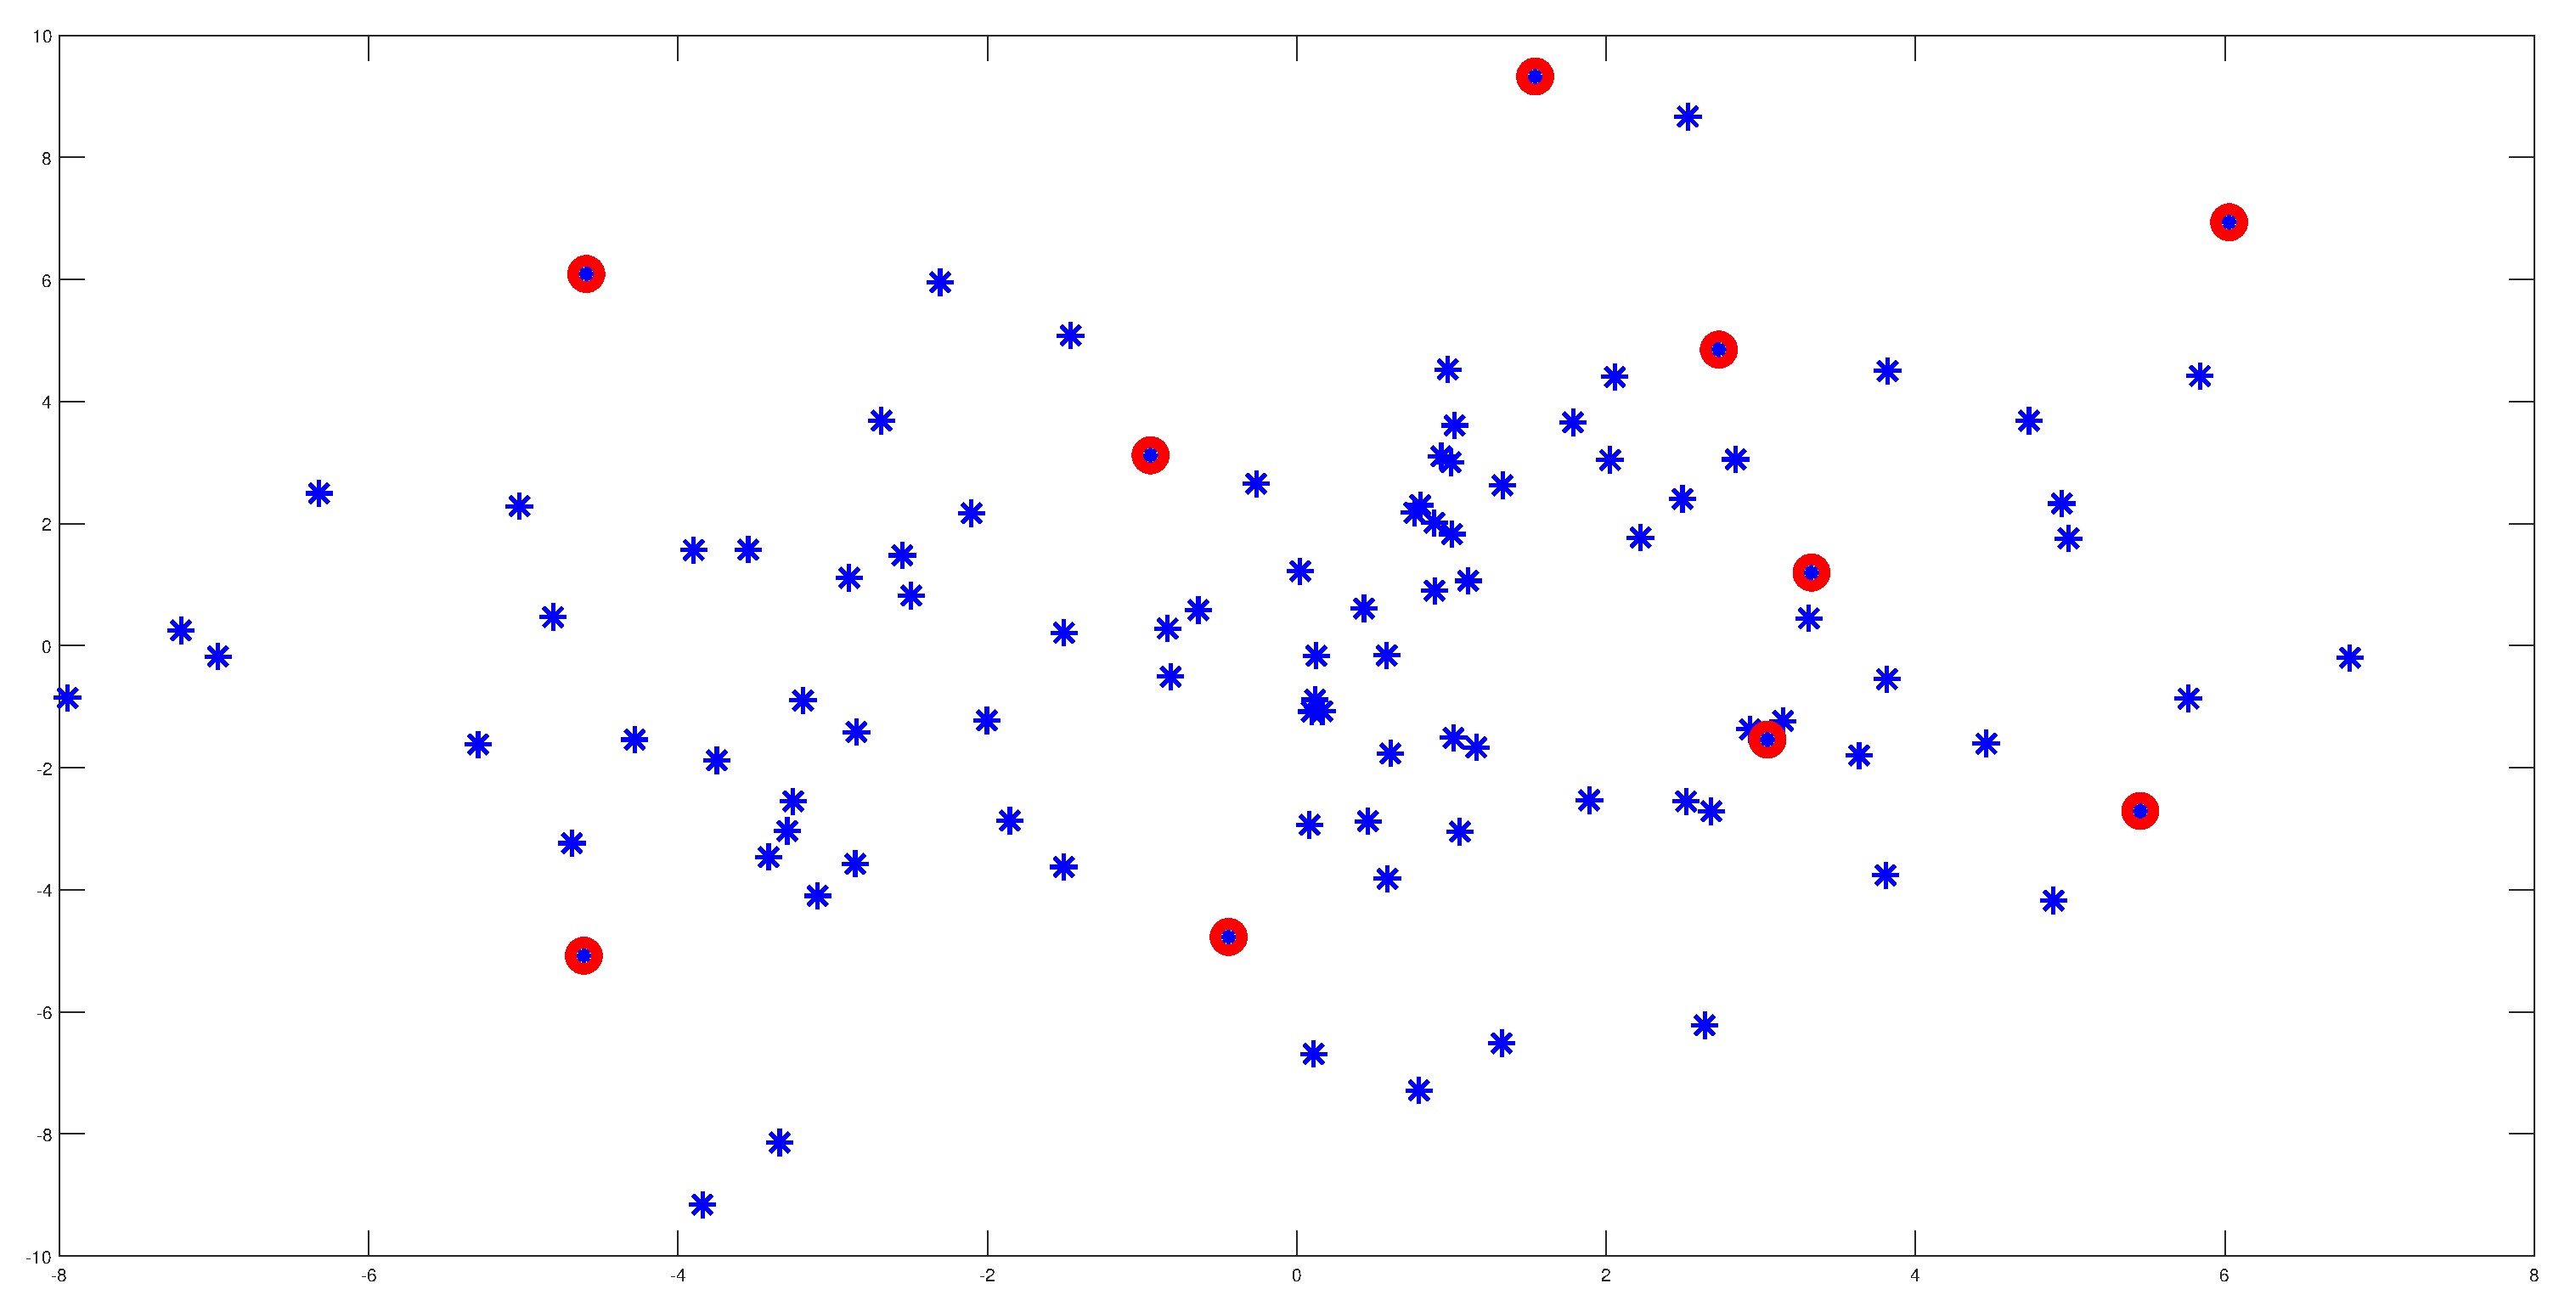
\includegraphics[height= 0.65\textwidth, width = 0.9\textwidth]{Exercise3/Report/fixed_lssvm_sig_0.1}
		\caption{$\sigma^2 = 0.1$}\label{fig:fixed_lssvm_sig_0.1}
	\end{subfigure}%
	\begin{subfigure}[b]{0.25\textwidth}
		\centering
		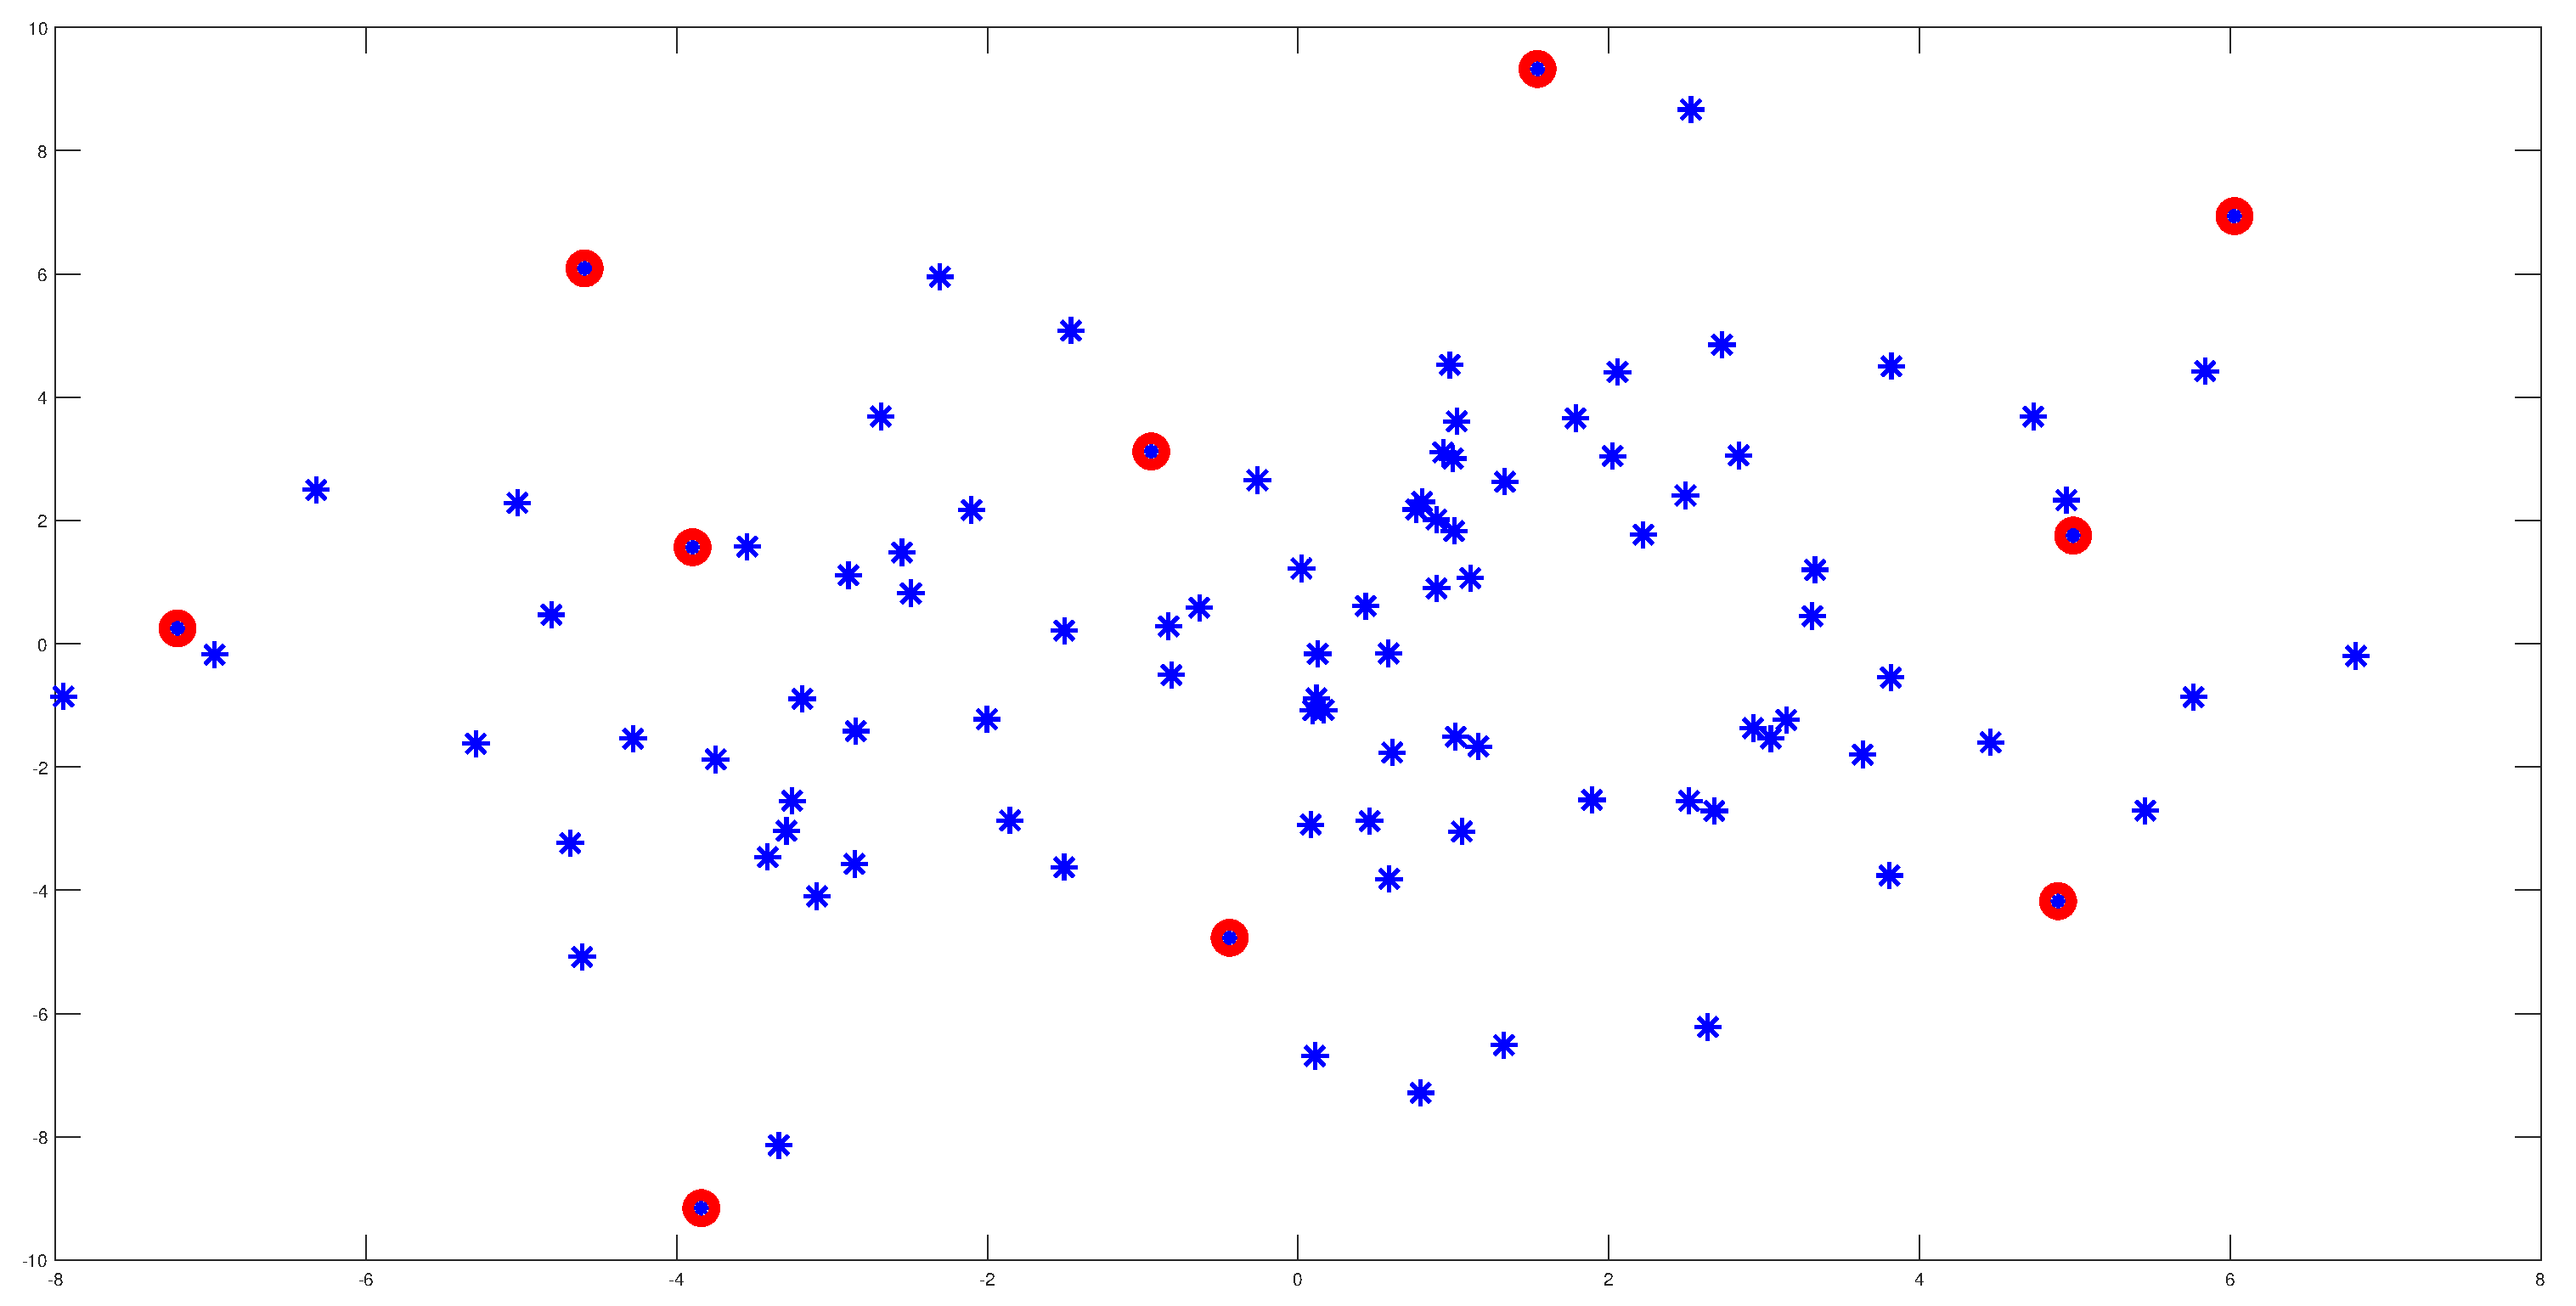
\includegraphics[height= 0.65\textwidth, width = 0.9\textwidth]{Exercise3/Report/fixed_lssvm_sig_1}
		\caption{$\sigma^2 = 1$}\label{fig:fixed_lssvm_sig_1}
	\end{subfigure}%
	\begin{subfigure}[b]{0.25\textwidth}
		\centering
		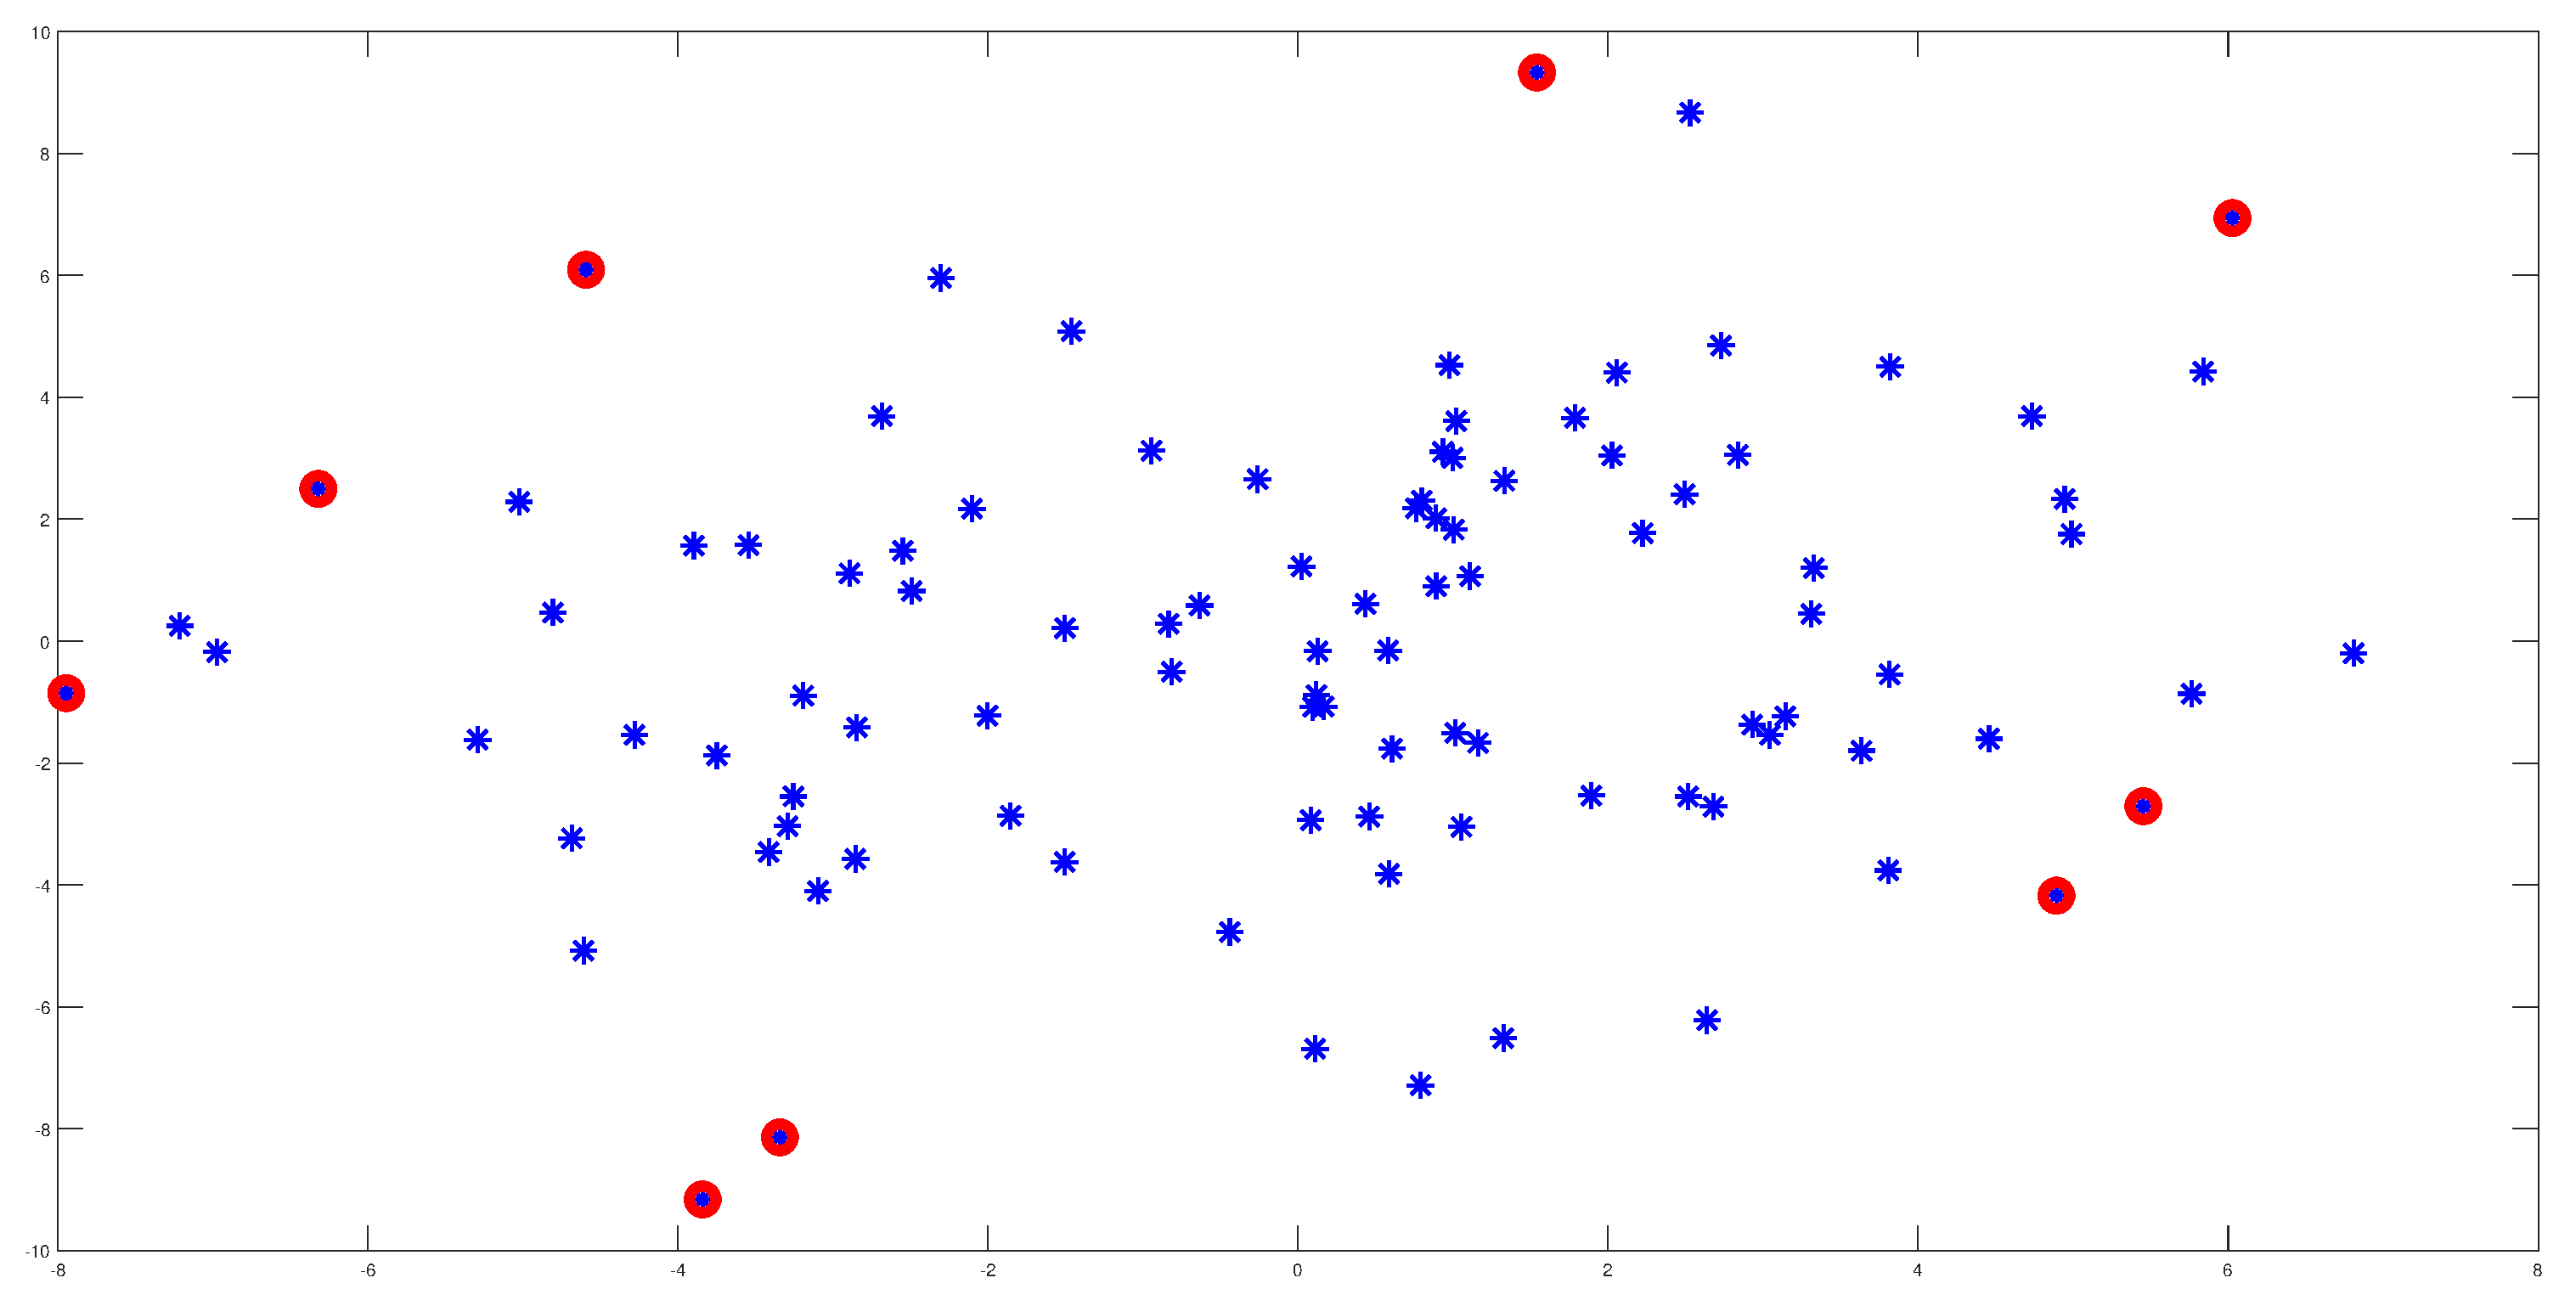
\includegraphics[height= 0.65\textwidth, width = 0.9\textwidth]{Exercise3/Report/fixed_lssvm_sig_100}
		\caption{$\sigma^2 = 100$}\label{fig:fixed_lssvm_sig_100}
	\end{subfigure}%
	\caption{Fixed-size LS-SVM for a two dimensional problem using
		RBF kernel}
	\label{fig:fixedlssvm}
\end{figure}\\\\
\textbf{Run fslssvm script.m. Use the Wisconsin Breast Cancer dataset for this exercise. Compare the results of fixed-size LS-SVM to $l_0$-approximation in terms of test errors, number of support vectors and computational time.}

In this exercise we compare the results of FS-LSSVM with $l_0$ approximation using breast cancer dataset. The error estimates for both the methods remains same without any variability as seen from the figure \ref{fig:Ex3_3.3_1}. The number of support vectors also remain the same. From figure \ref{fig:Ex3_3.3_3}, it can seen that FS-LSSVM takes lesser computations compared to $l_0$ approximation, but FS-LSSVM has higher variability than $l_0$.
\begin{figure}[!htpb]
	\begin{subfigure}[b]{0.34\textwidth}
		\centering
		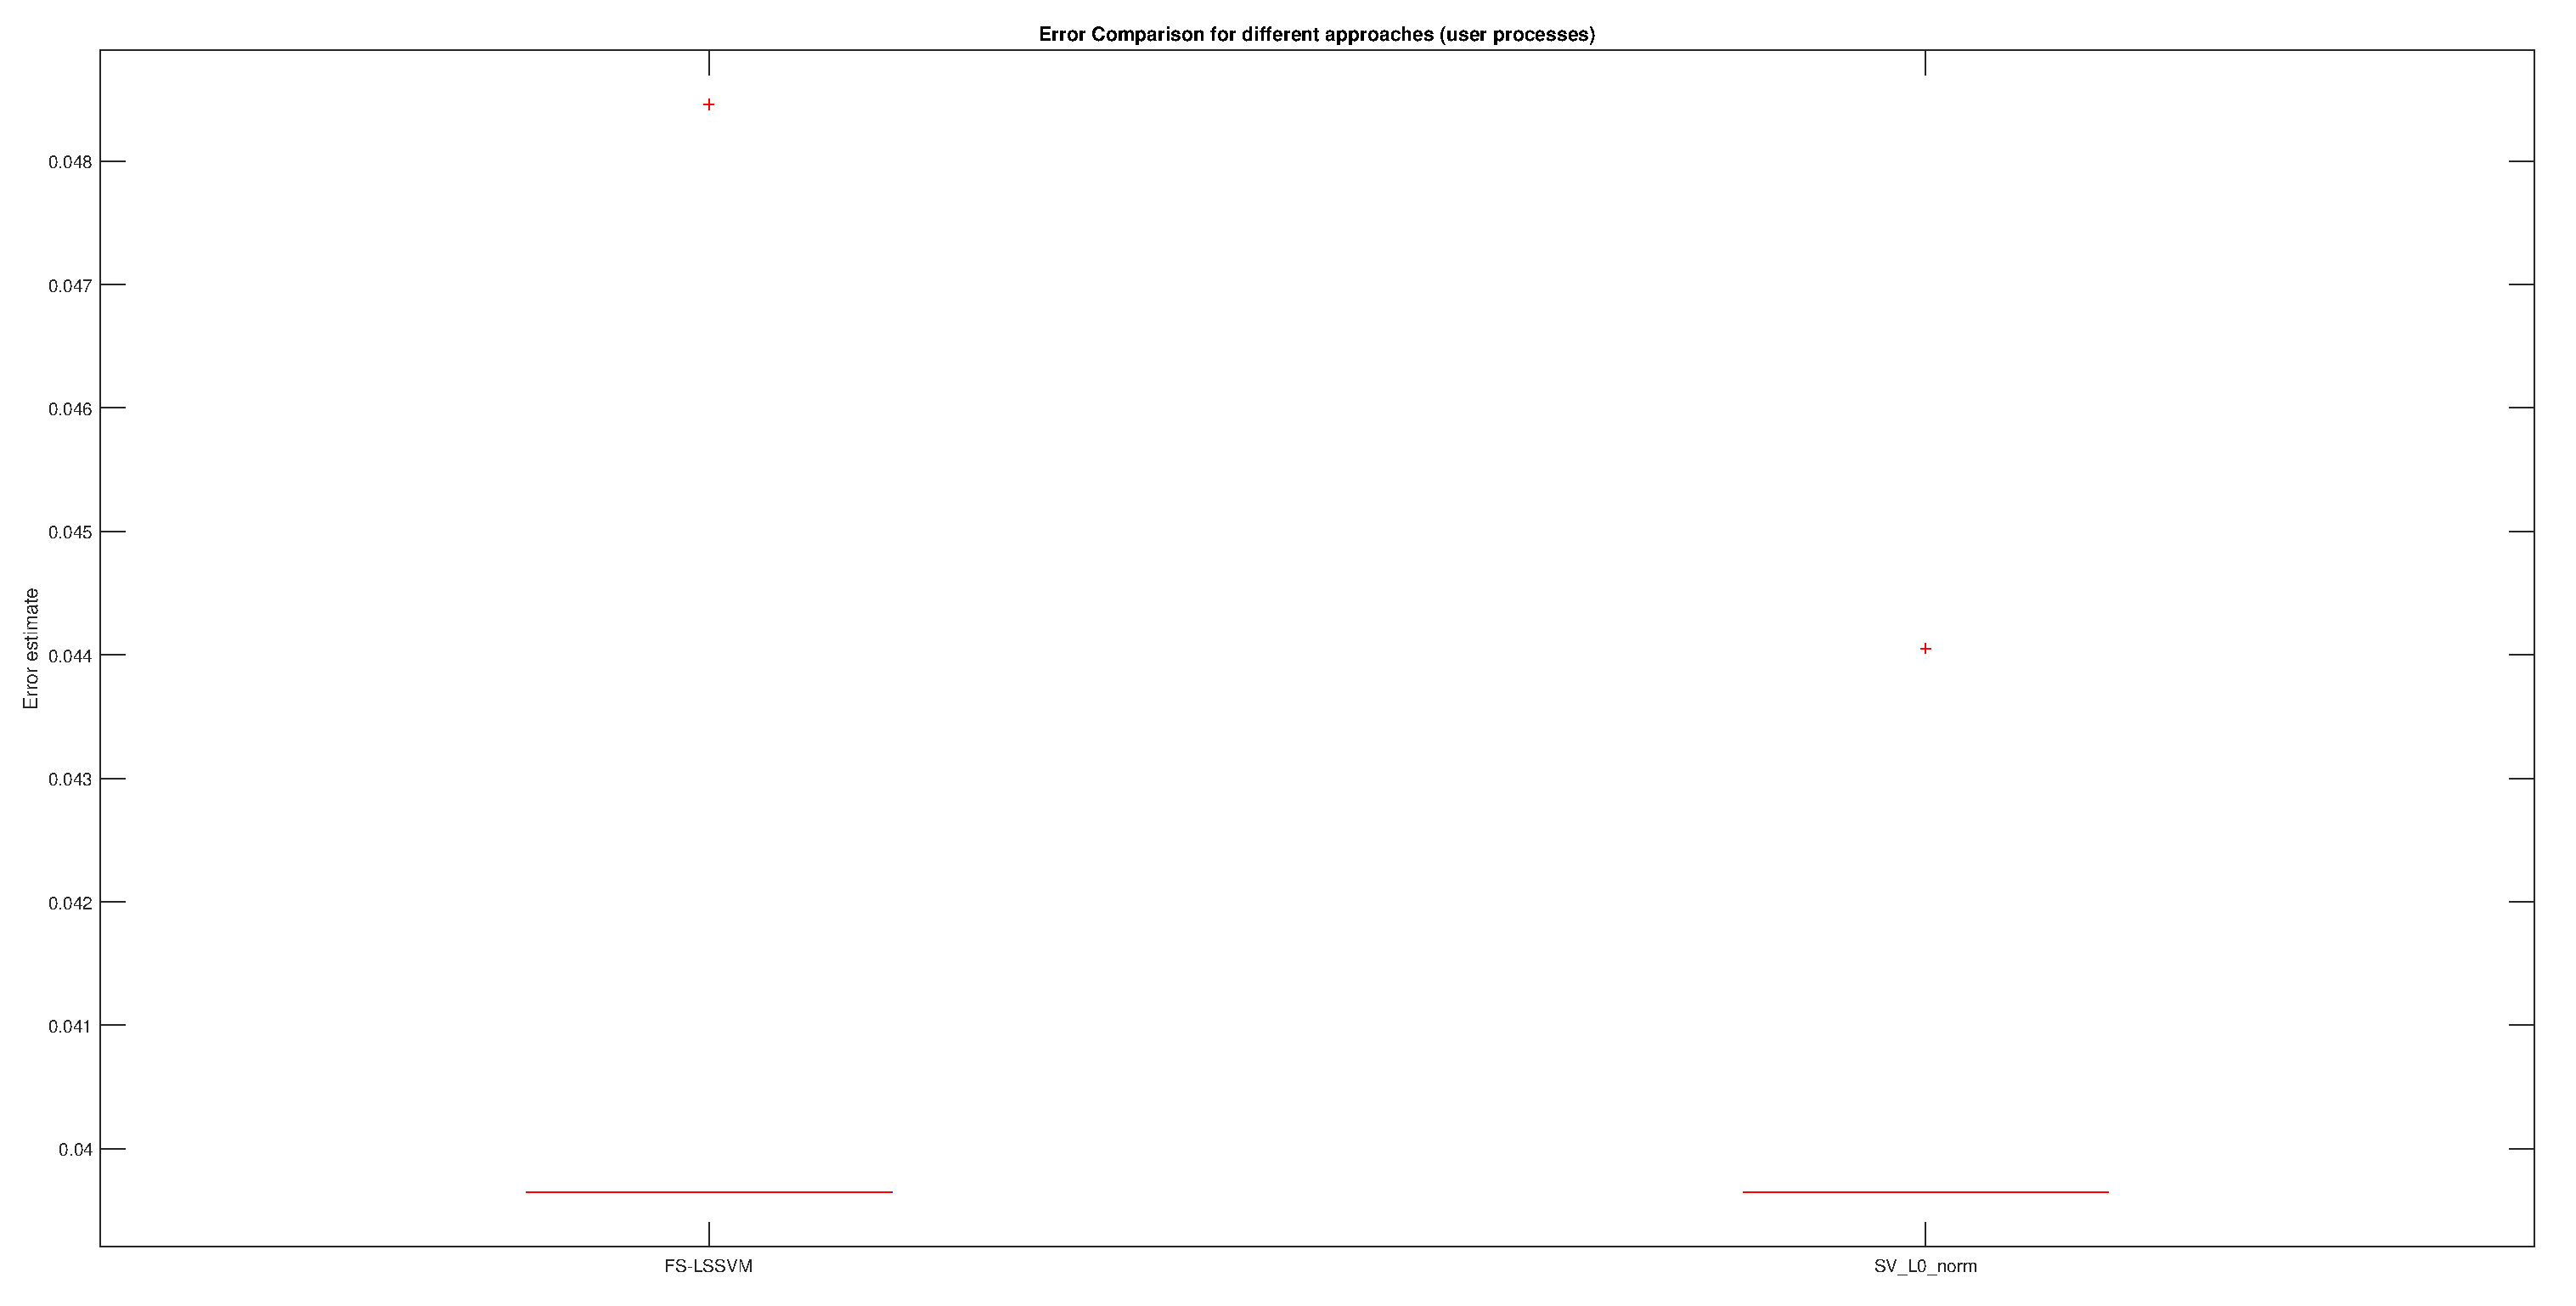
\includegraphics[height= 0.65\textwidth, width = 0.8\textwidth]{Exercise3/Report/Ex3_3.3_1.eps}
		\caption{Error estimates }\label{fig:Ex3_3.3_1}
	\end{subfigure}%
	\begin{subfigure}[b]{0.34\textwidth}
		\centering
		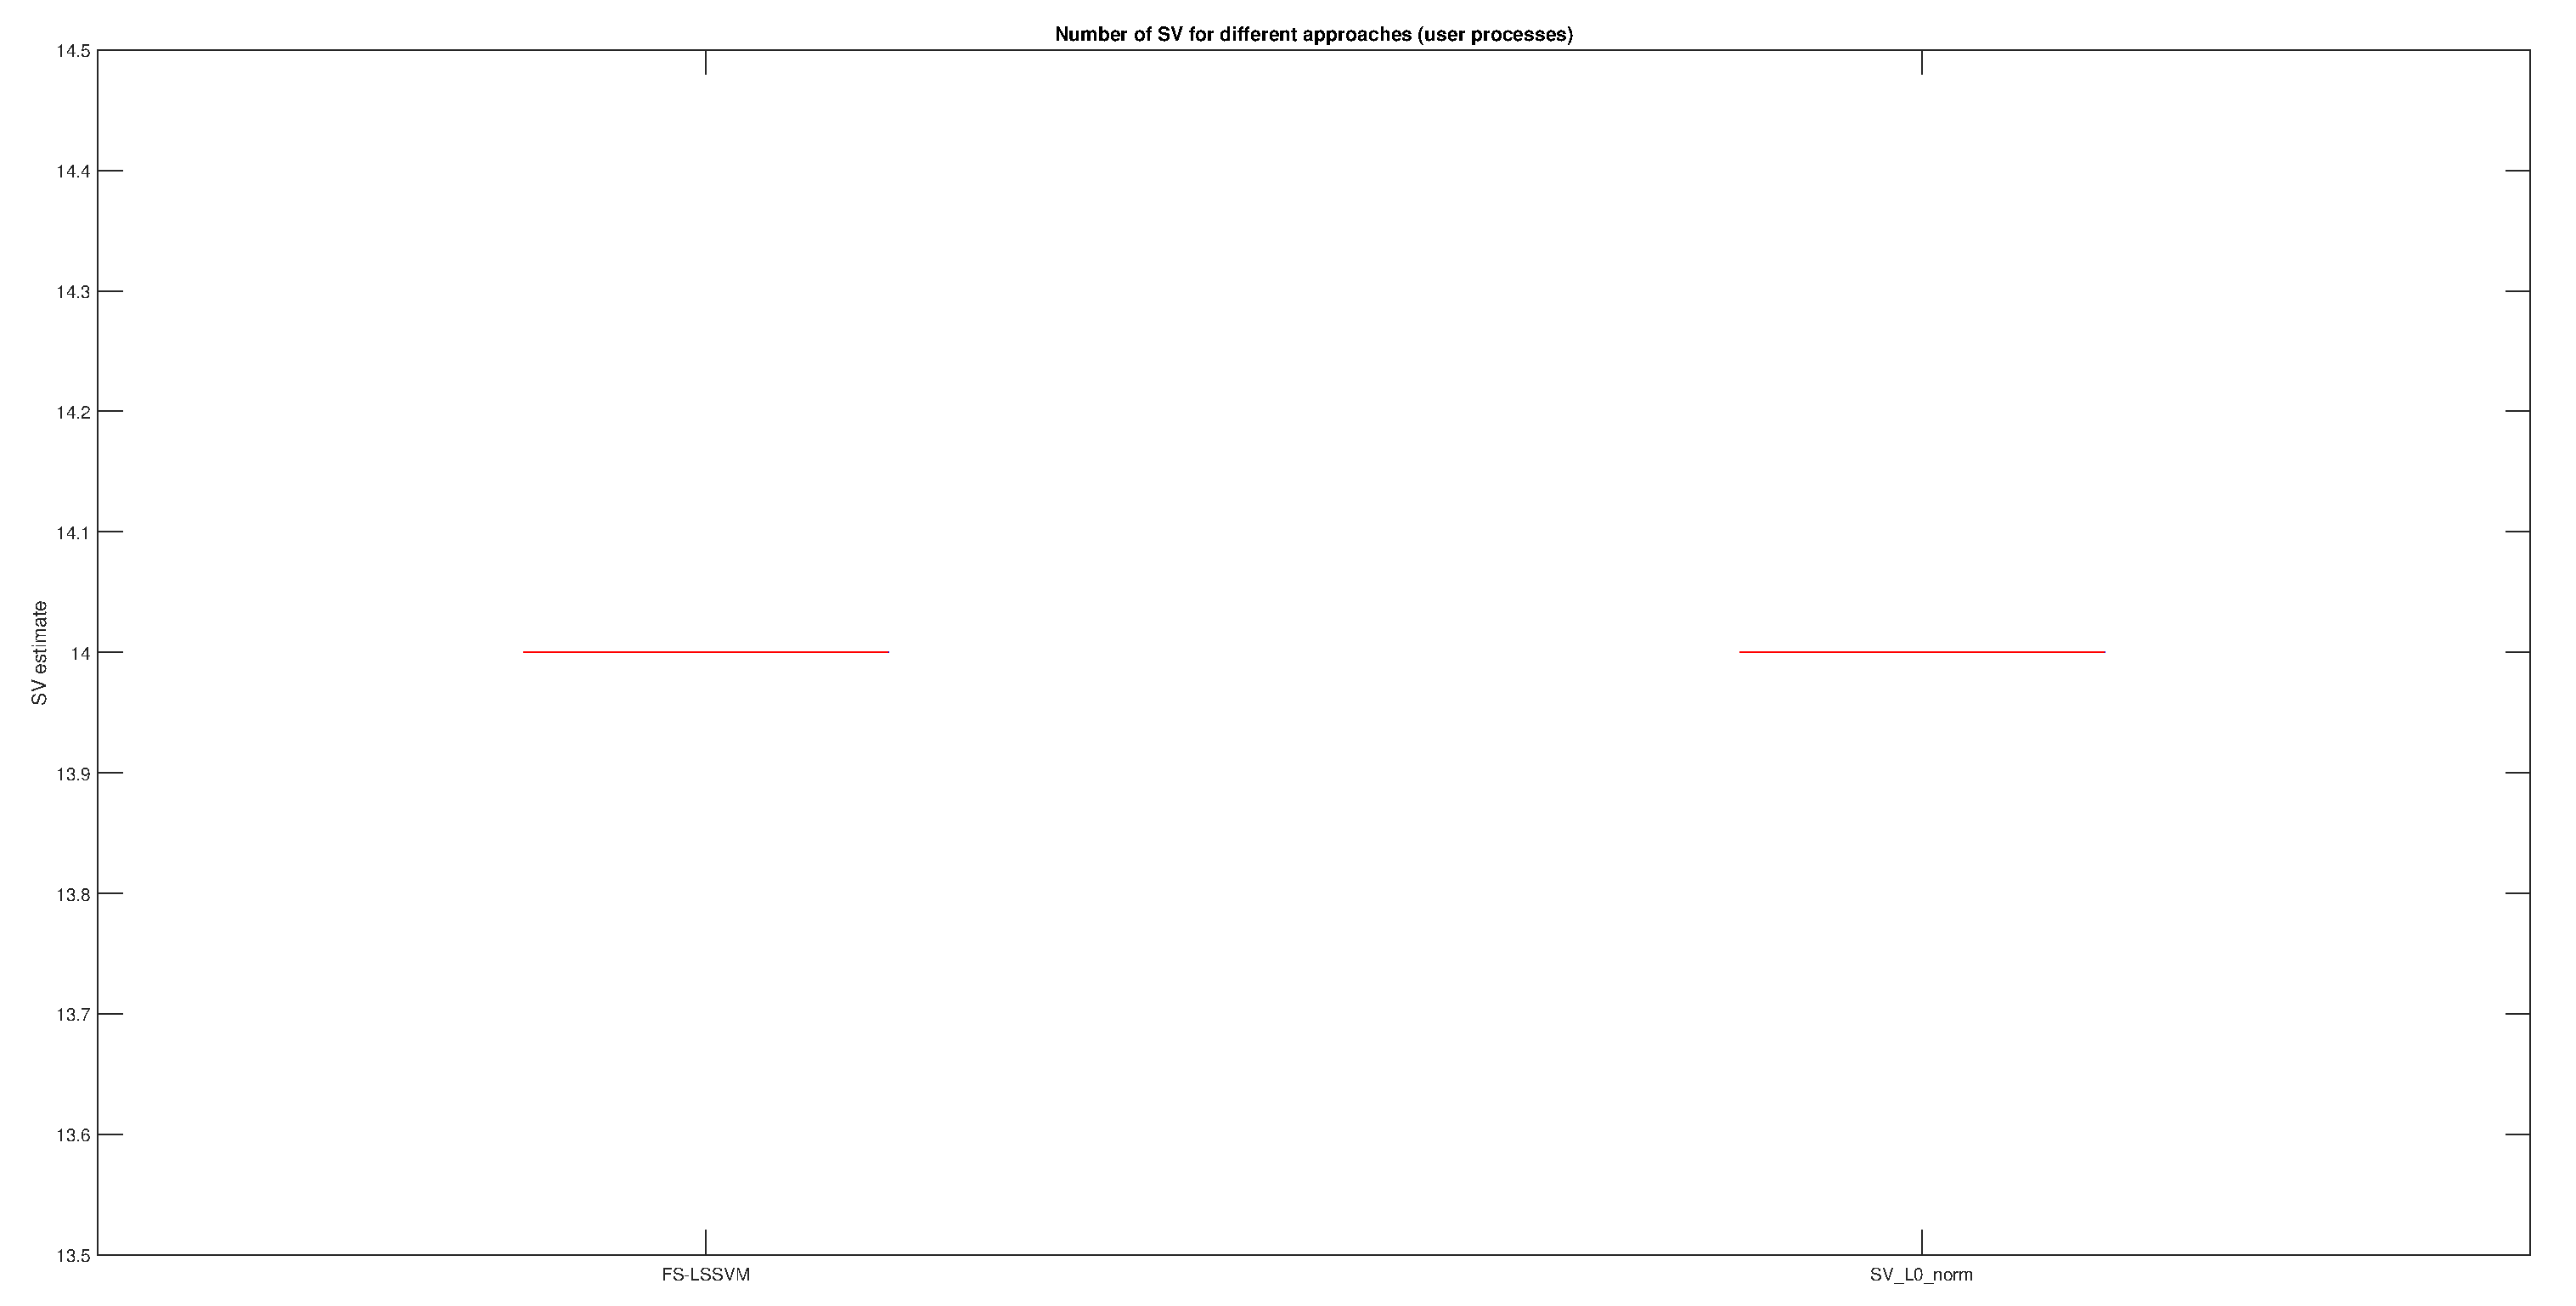
\includegraphics[height= 0.65\textwidth, width = 0.8\textwidth]{Exercise3/Report/Ex3_3.3_2.eps}
		\caption{Number of Support Vectors}\label{fig:Ex3_3.3_2}
	\end{subfigure}%
	\begin{subfigure}[b]{0.34\textwidth}
		\centering
		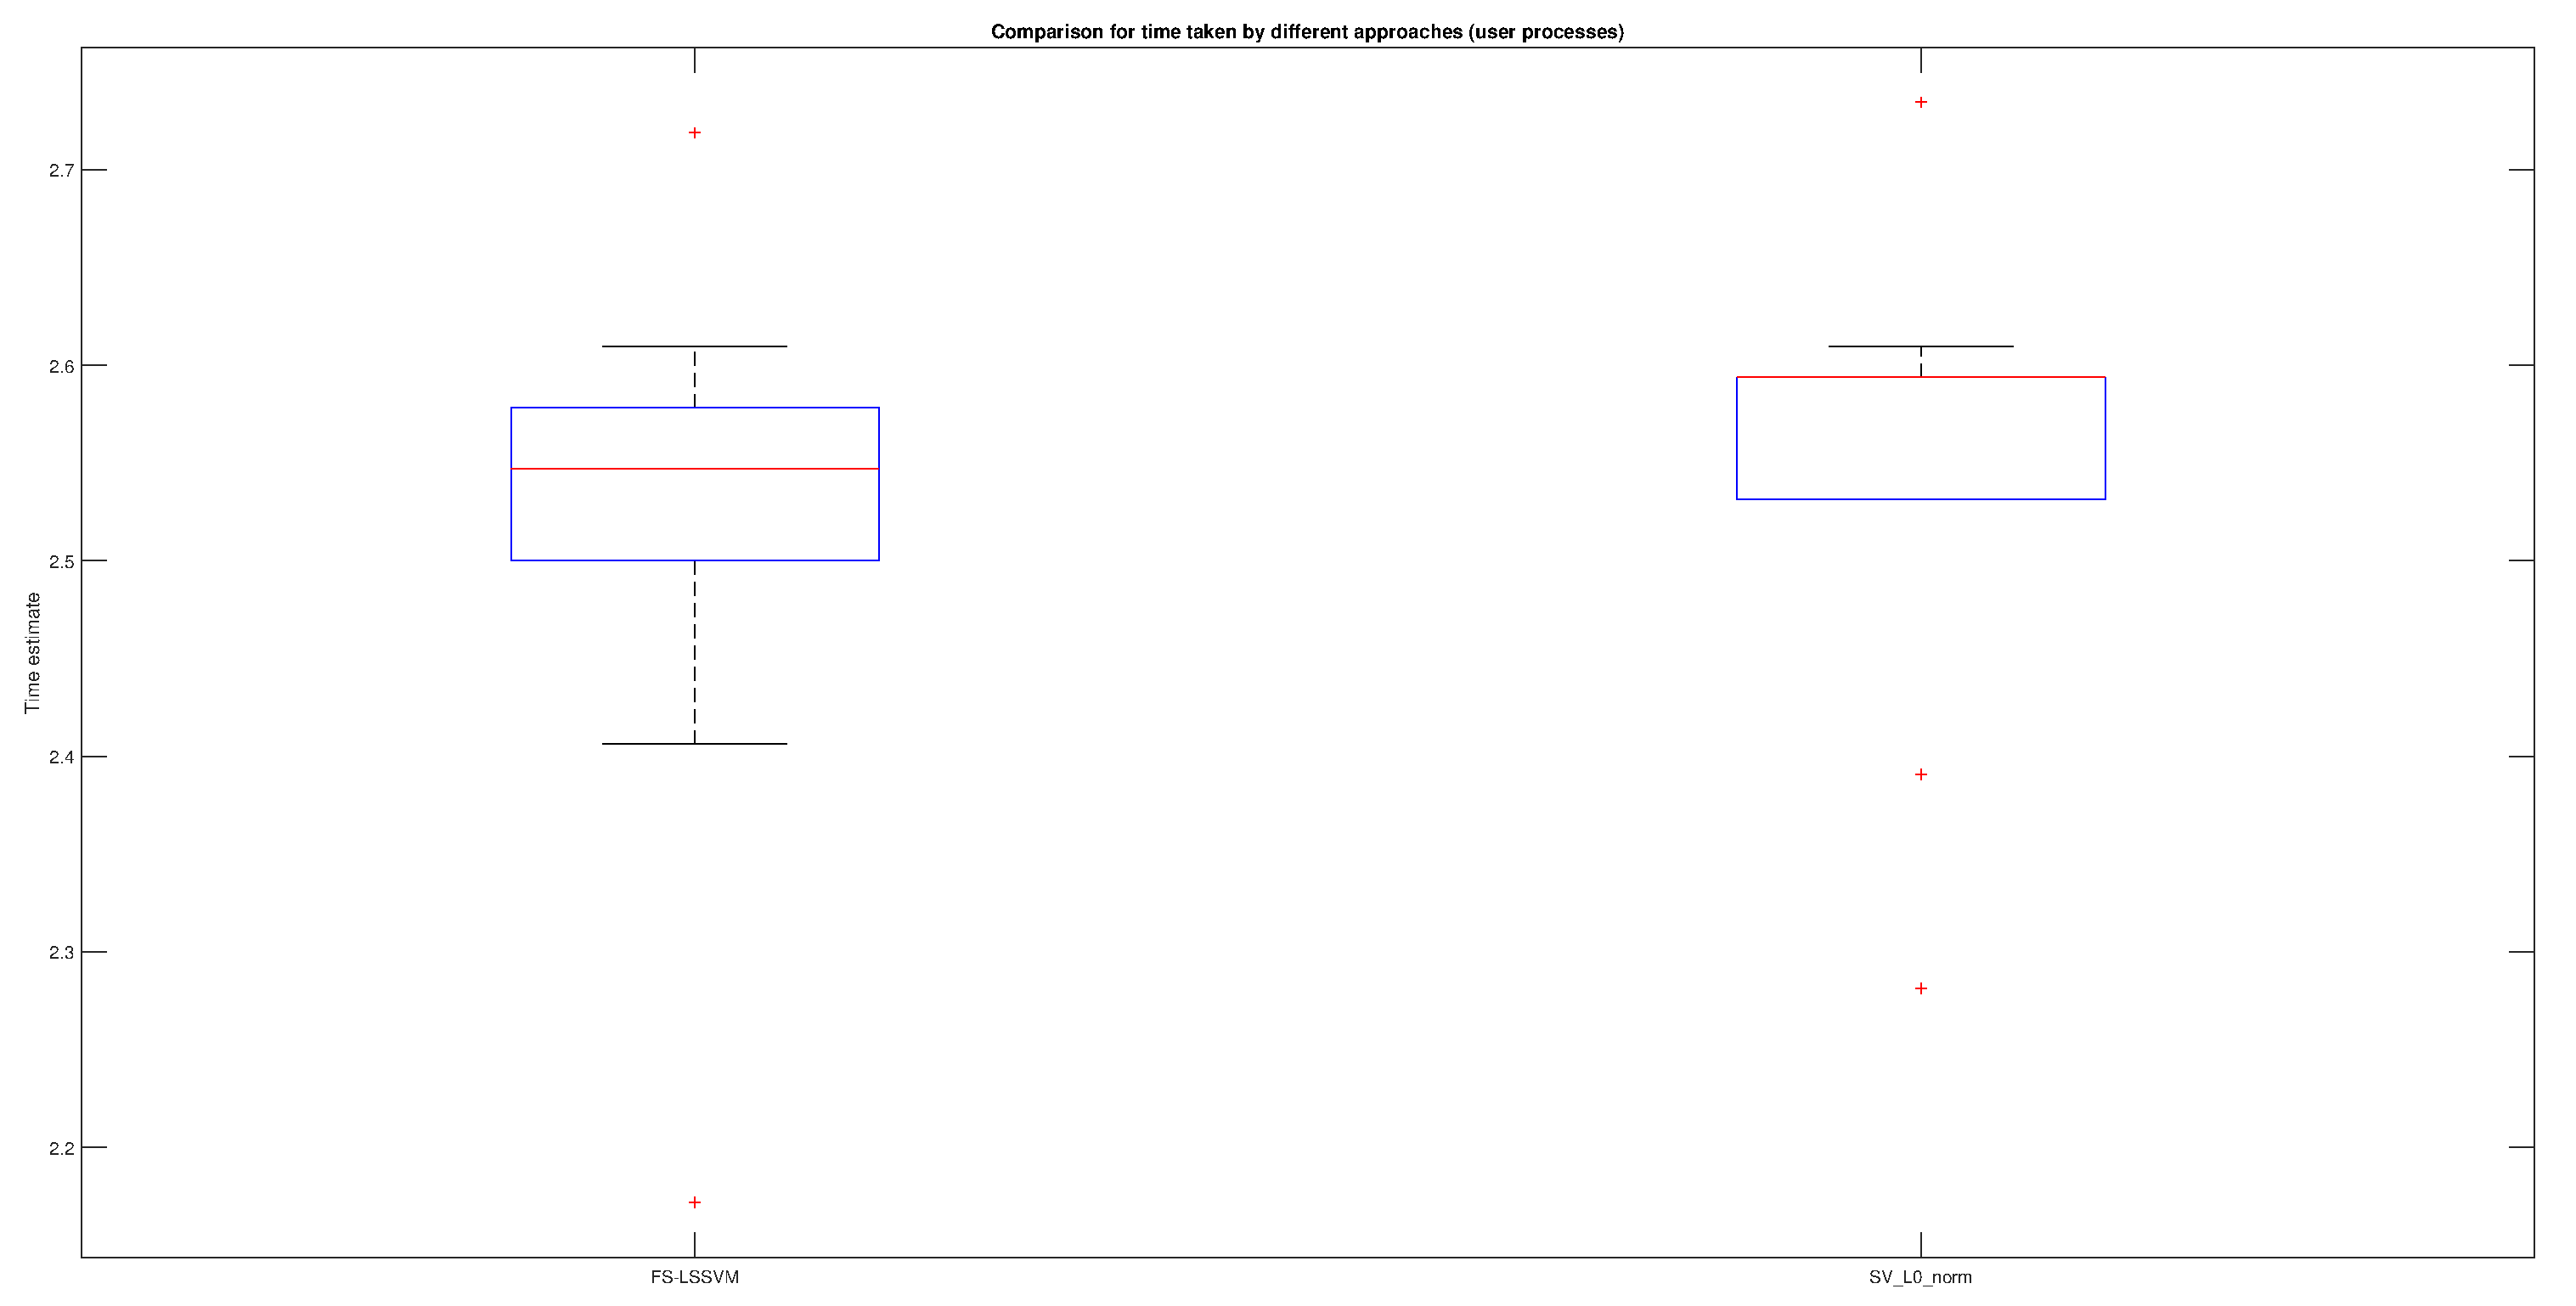
\includegraphics[height= 0.65\textwidth, width = 0.8\textwidth]{Exercise3/Report/Ex3_3.3_3.eps}
		\caption{Computation Time}\label{fig:Ex3_3.3_3}
	\end{subfigure}%
	\caption{Breast Cancer Dataset; Fixed Size - LSSVM vs $l_0$ - type approximation}
	\label{fig:Ex3_3.3}
\end{figure}
\section{Homework Problems}
\subsection{Kernel principal component analysis}
We run the provided script for denoising the digit images with a noise level of 1.0 and the results are plotted in the figure \ref{fig:dig_denoise} for the models with linear and RBF kernels. It can be seen that the model with RBF kernel does a good job in denoising the noisy images. For number of PC's = 16 and above, the model denoises the original images from noisy ones except for the the digit 7 where it decodes it as digit 2. Linear kernel on the other hand does a very poor job for higher principal components and the denoised images are more or less noisy. 
\begin{figure}[!htpb]
	\begin{subfigure}[b]{0.4\textwidth}
		\centering
		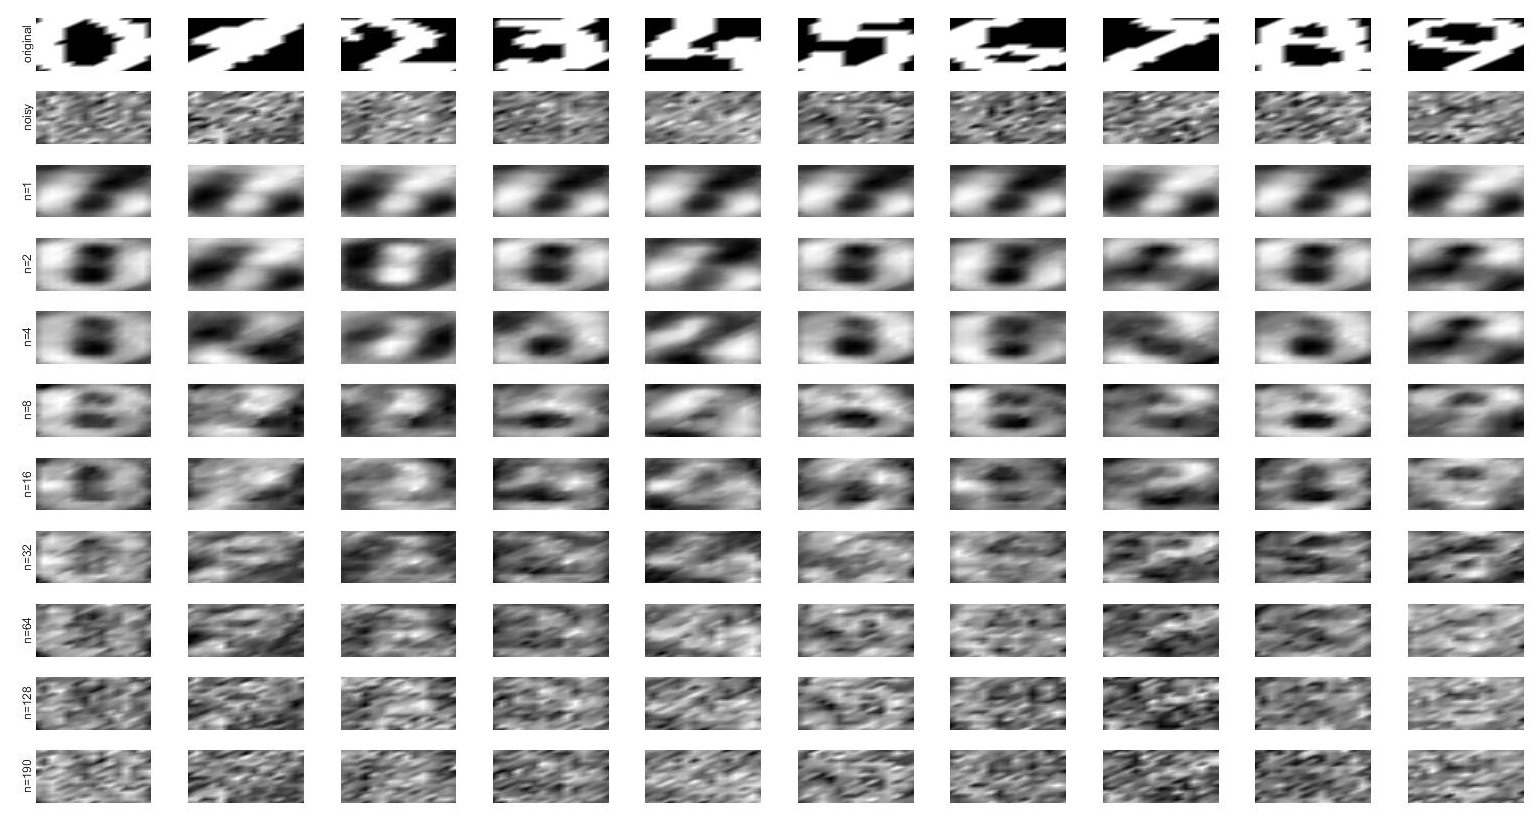
\includegraphics[height= 0.75\textwidth, width = 0.9\textwidth]{Exercise3/Report/dig_denoise_linear}
		\caption{Noise Level: 1.0 - Linear Kernel }\label{fig:dig_denoise_linear}
	\end{subfigure}%
	\begin{subfigure}[b]{0.4\textwidth}
		\centering
		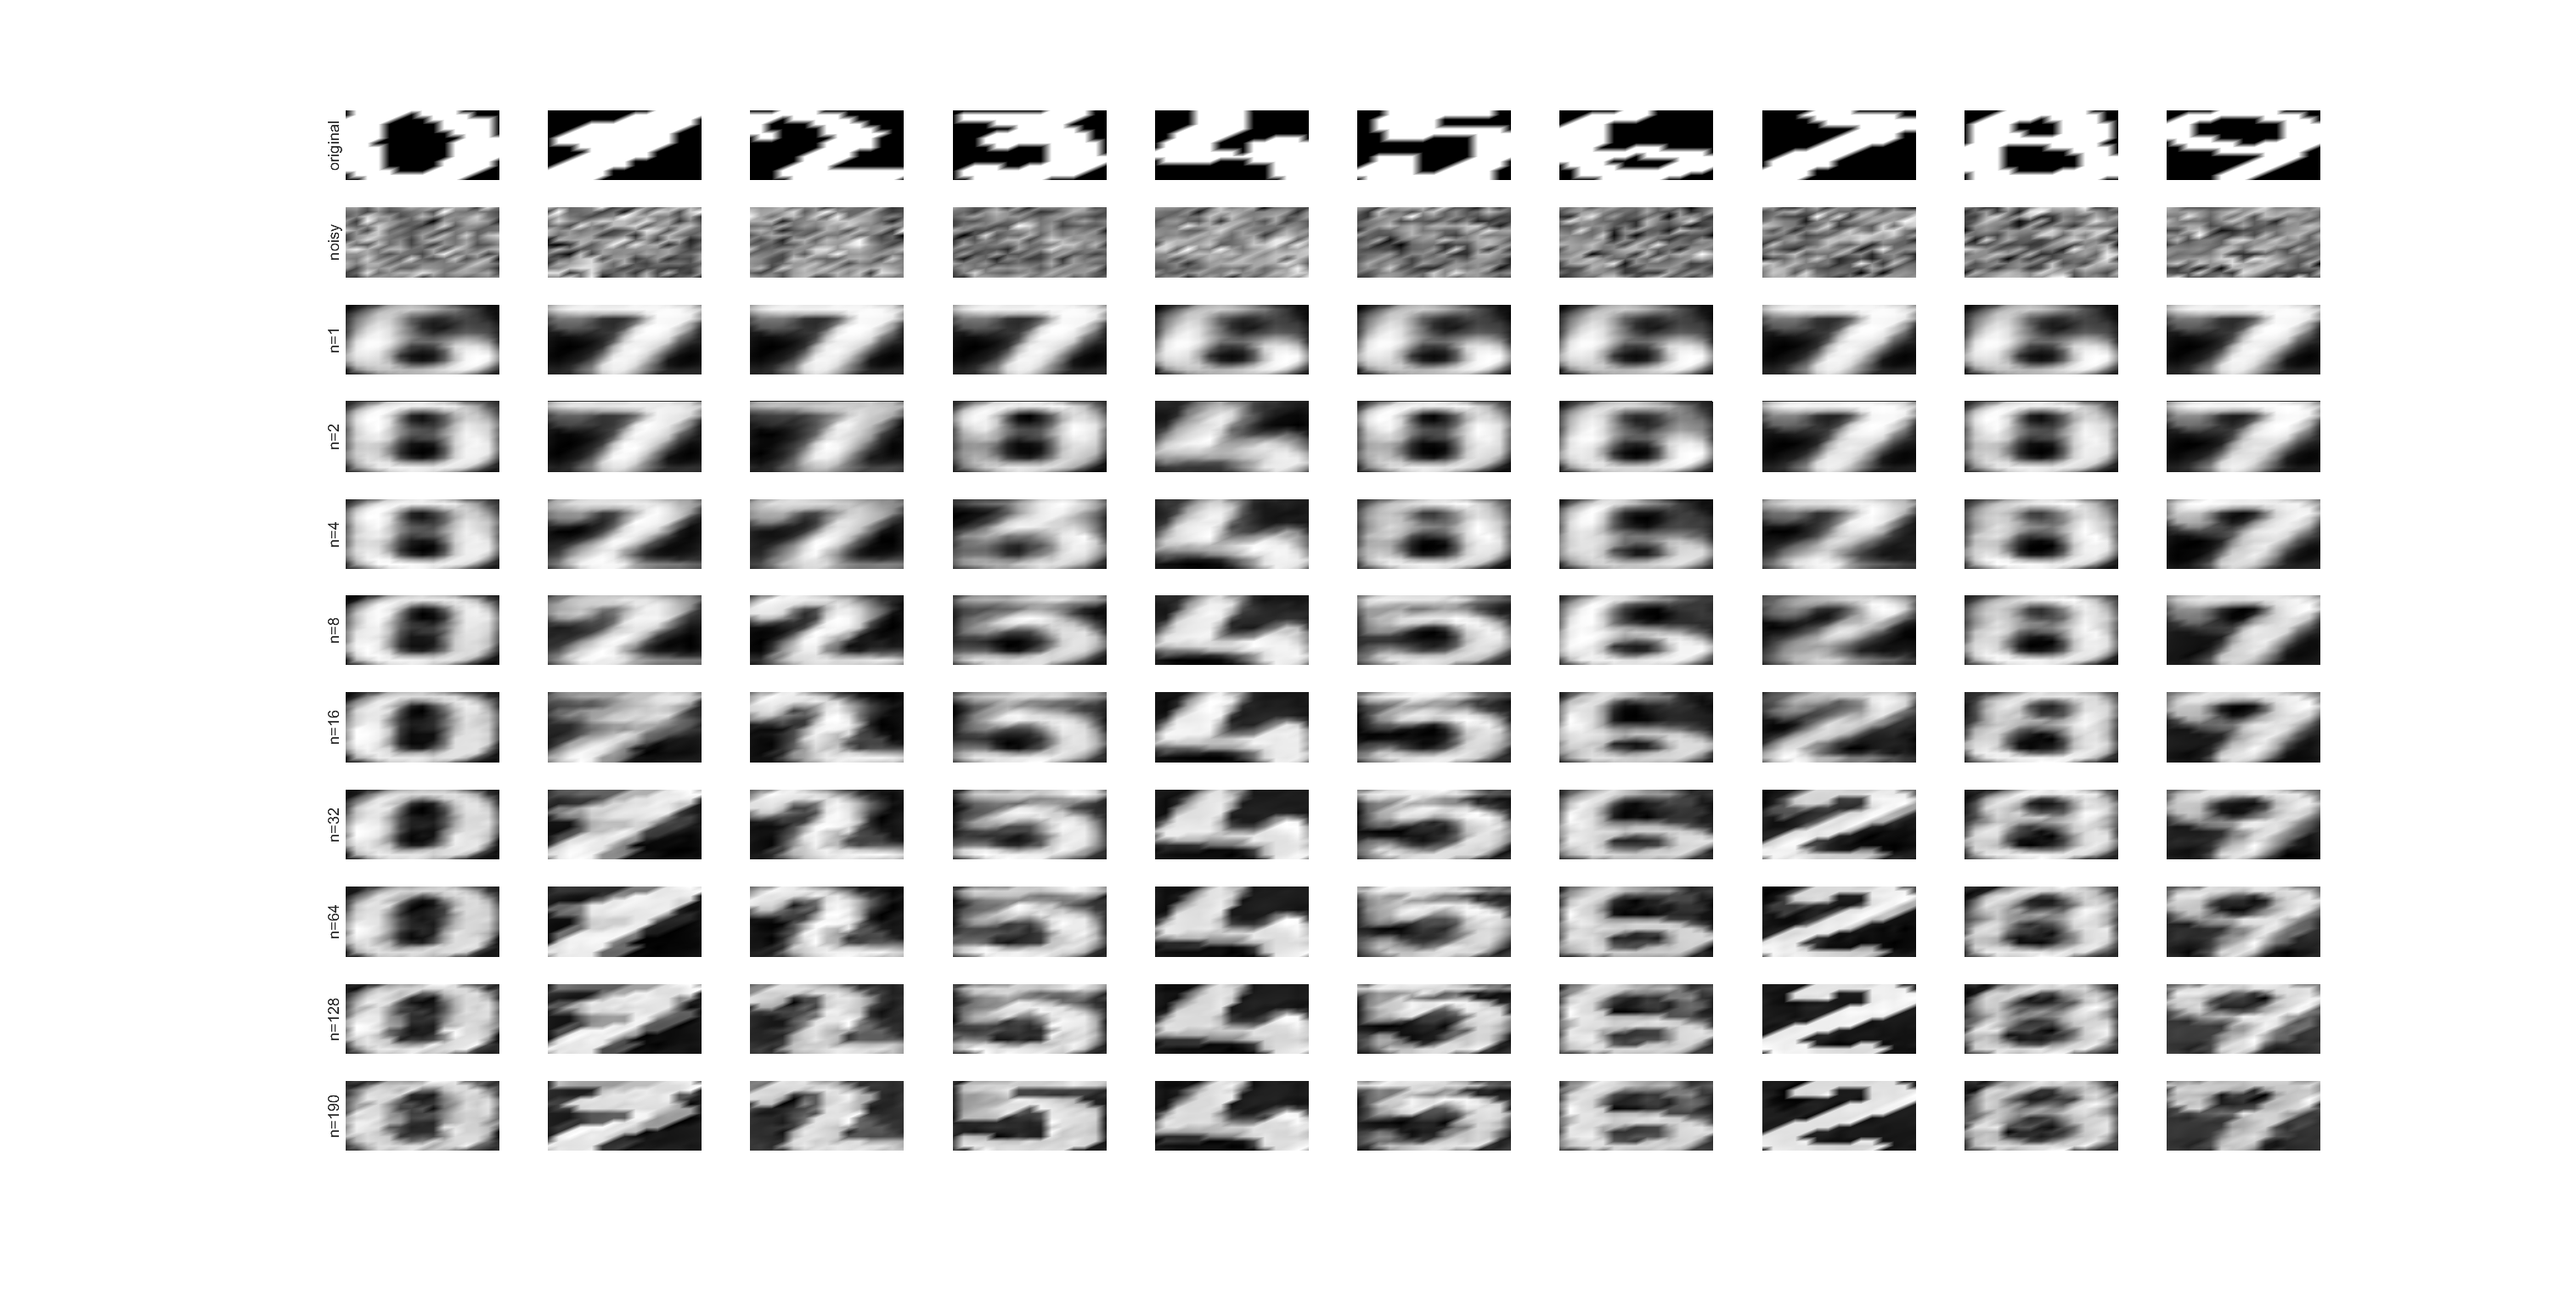
\includegraphics[height= 0.75\textwidth, width = 0.9\textwidth]{Exercise3/Report/dig_denoise_rbf}
		\caption{Noise Level: 1.0 - RBF Kernel}\label{fig:dig_denoise_rbf}
	\end{subfigure}%
	\caption{Digit denoising using RBF and Linear Kernels}
	\label{fig:dig_denoise}
\end{figure}
In the script the default settings has a $\sigma^2$ value of 35. To analyze the effect of change in $\sigma^2$ we run the algorithm with multiples values such as (0.001;0.01;0.1;1;10;100) and some of the results are shown in the figure \ref{fig:dig_denoise_rbf_sig}. From the figure it can be seen that for values 0.1 and 1, the denoising of images from noisy data is clear with only few wrong images (digit 3, 5, 9). As the $\sigma^2$ increases, the denoised images tend to be more nosier as the reconstruction error is high and the output resembles the one similar to a linear kernel.  
\begin{figure}[!htpb]
	\begin{subfigure}[b]{0.25\textwidth}
		\centering
		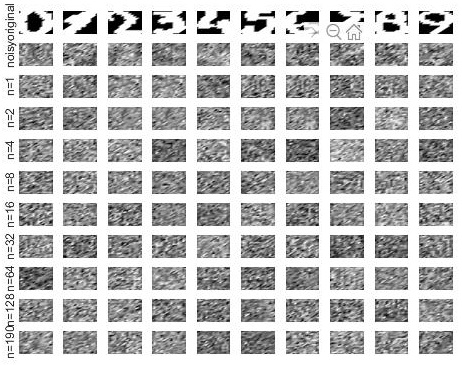
\includegraphics[height= 0.75\textwidth, width = 0.95\textwidth]{Exercise3/Report/dig_denoise_rbf_sig_0.1}
		\caption{$\sigma^2 = 0.001$ }\label{fig:dig_denoise_rbf_sig_0.1}
	\end{subfigure}%
	\begin{subfigure}[b]{0.25\textwidth}
		\centering
		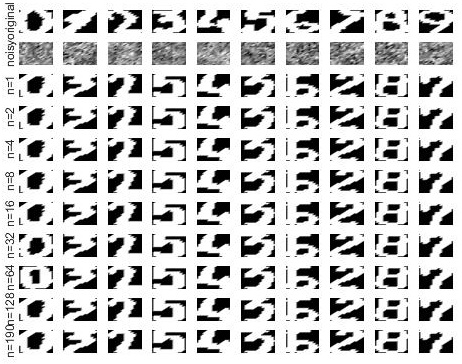
\includegraphics[height= 0.75\textwidth, width = 0.95\textwidth]{Exercise3/Report/dig_denoise_rbf_sig_1}
		\caption{$\sigma^2 = 0.1$}\label{fig:dig_denoise_rbf_sig_1}
	\end{subfigure}%
	\begin{subfigure}[b]{0.25\textwidth}
		\centering
		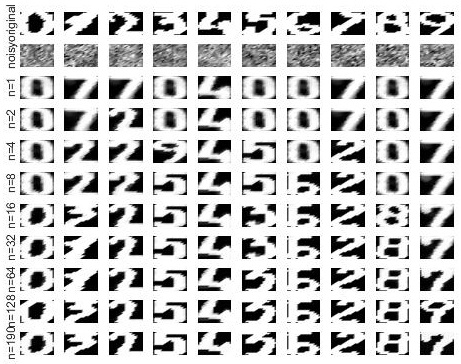
\includegraphics[height= 0.75\textwidth, width = 0.95\textwidth]{Exercise3/Report/dig_denoise_rbf_sig_10}
		\caption{$\sigma^2 = 1$}\label{fig:dig_denoise_rbf_sig_10}
	\end{subfigure}%
	\begin{subfigure}[b]{0.25\textwidth}
		\centering
		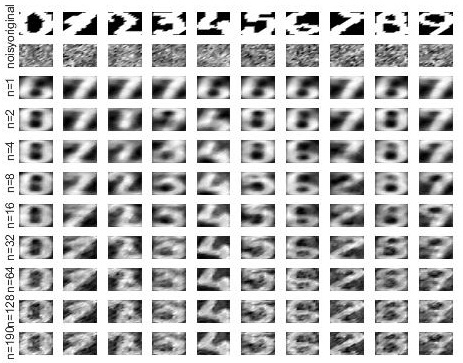
\includegraphics[height= 0.75\textwidth, width = 0.95\textwidth]{Exercise3/Report/dig_denoise_rbf_sig_100}
		\caption{$\sigma^2 = 100$}\label{fig:dig_denoise_rbf_sig_100}
	\end{subfigure}%
	\caption{Digit Denoising with RBF kernel for various $\sigma^2$ values}
	\label{fig:dig_denoise_rbf_sig}
\end{figure}
\subsection{ Fixed-size LS-SVM}
\subsubsection{ Shuttle (statlog)}
The shuttle log dataset contains 700 data points with 9 features and 1 class. Fixed-size LS-SVM algorithm is run on this dataset and the results are plotted in the below figure \ref{fig:shuttle}. The error estimates is almost same for both the methods but Fixed-size LSSVM is has slight lower error by a value of 0.003. FS-LSSVM takes around 13 support vectors whereas $l_0$ -type method takes only 6 about one-third of FS-LSSVM method. Regarding the computational complexity, FS-LSSVM is faster and can be seen from figure \ref{fig:shuttle_3}. 
\begin{figure}[!htpb]
	\begin{subfigure}[b]{0.34\textwidth}
		\centering
		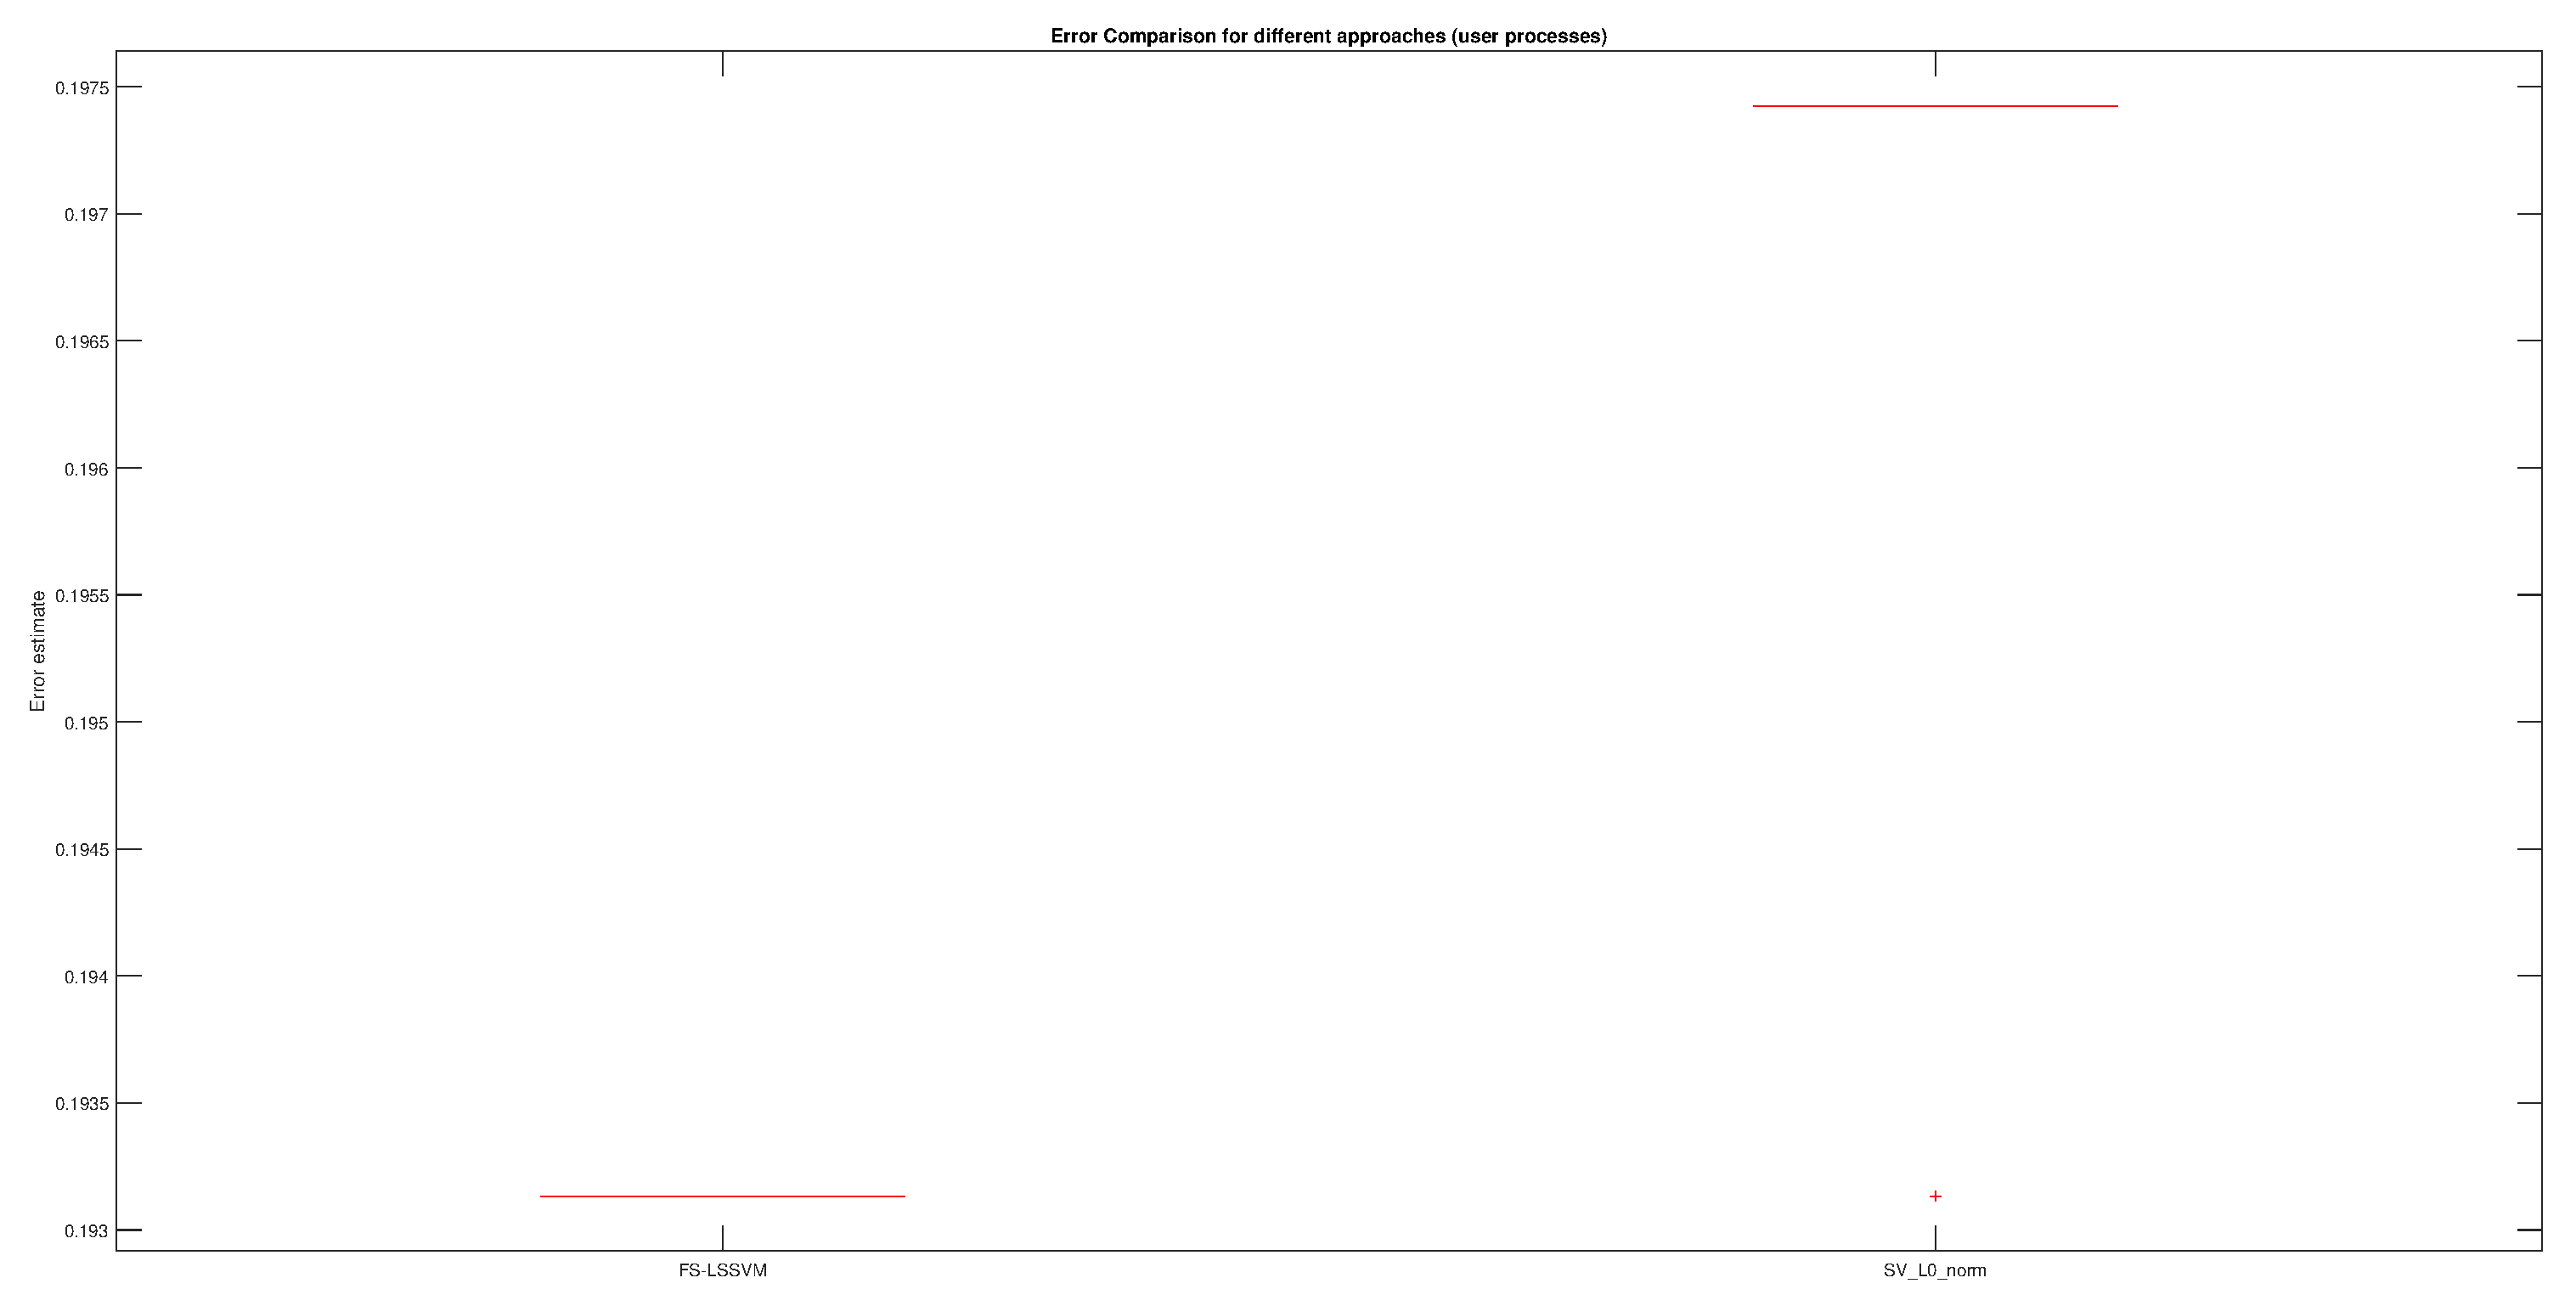
\includegraphics[height= 0.65\textwidth, width = 0.8\textwidth]{Exercise3/Report/shuttle_1}
		\caption{Error estimates }\label{fig:shuttle_1}
	\end{subfigure}%
	\begin{subfigure}[b]{0.34\textwidth}
		\centering
		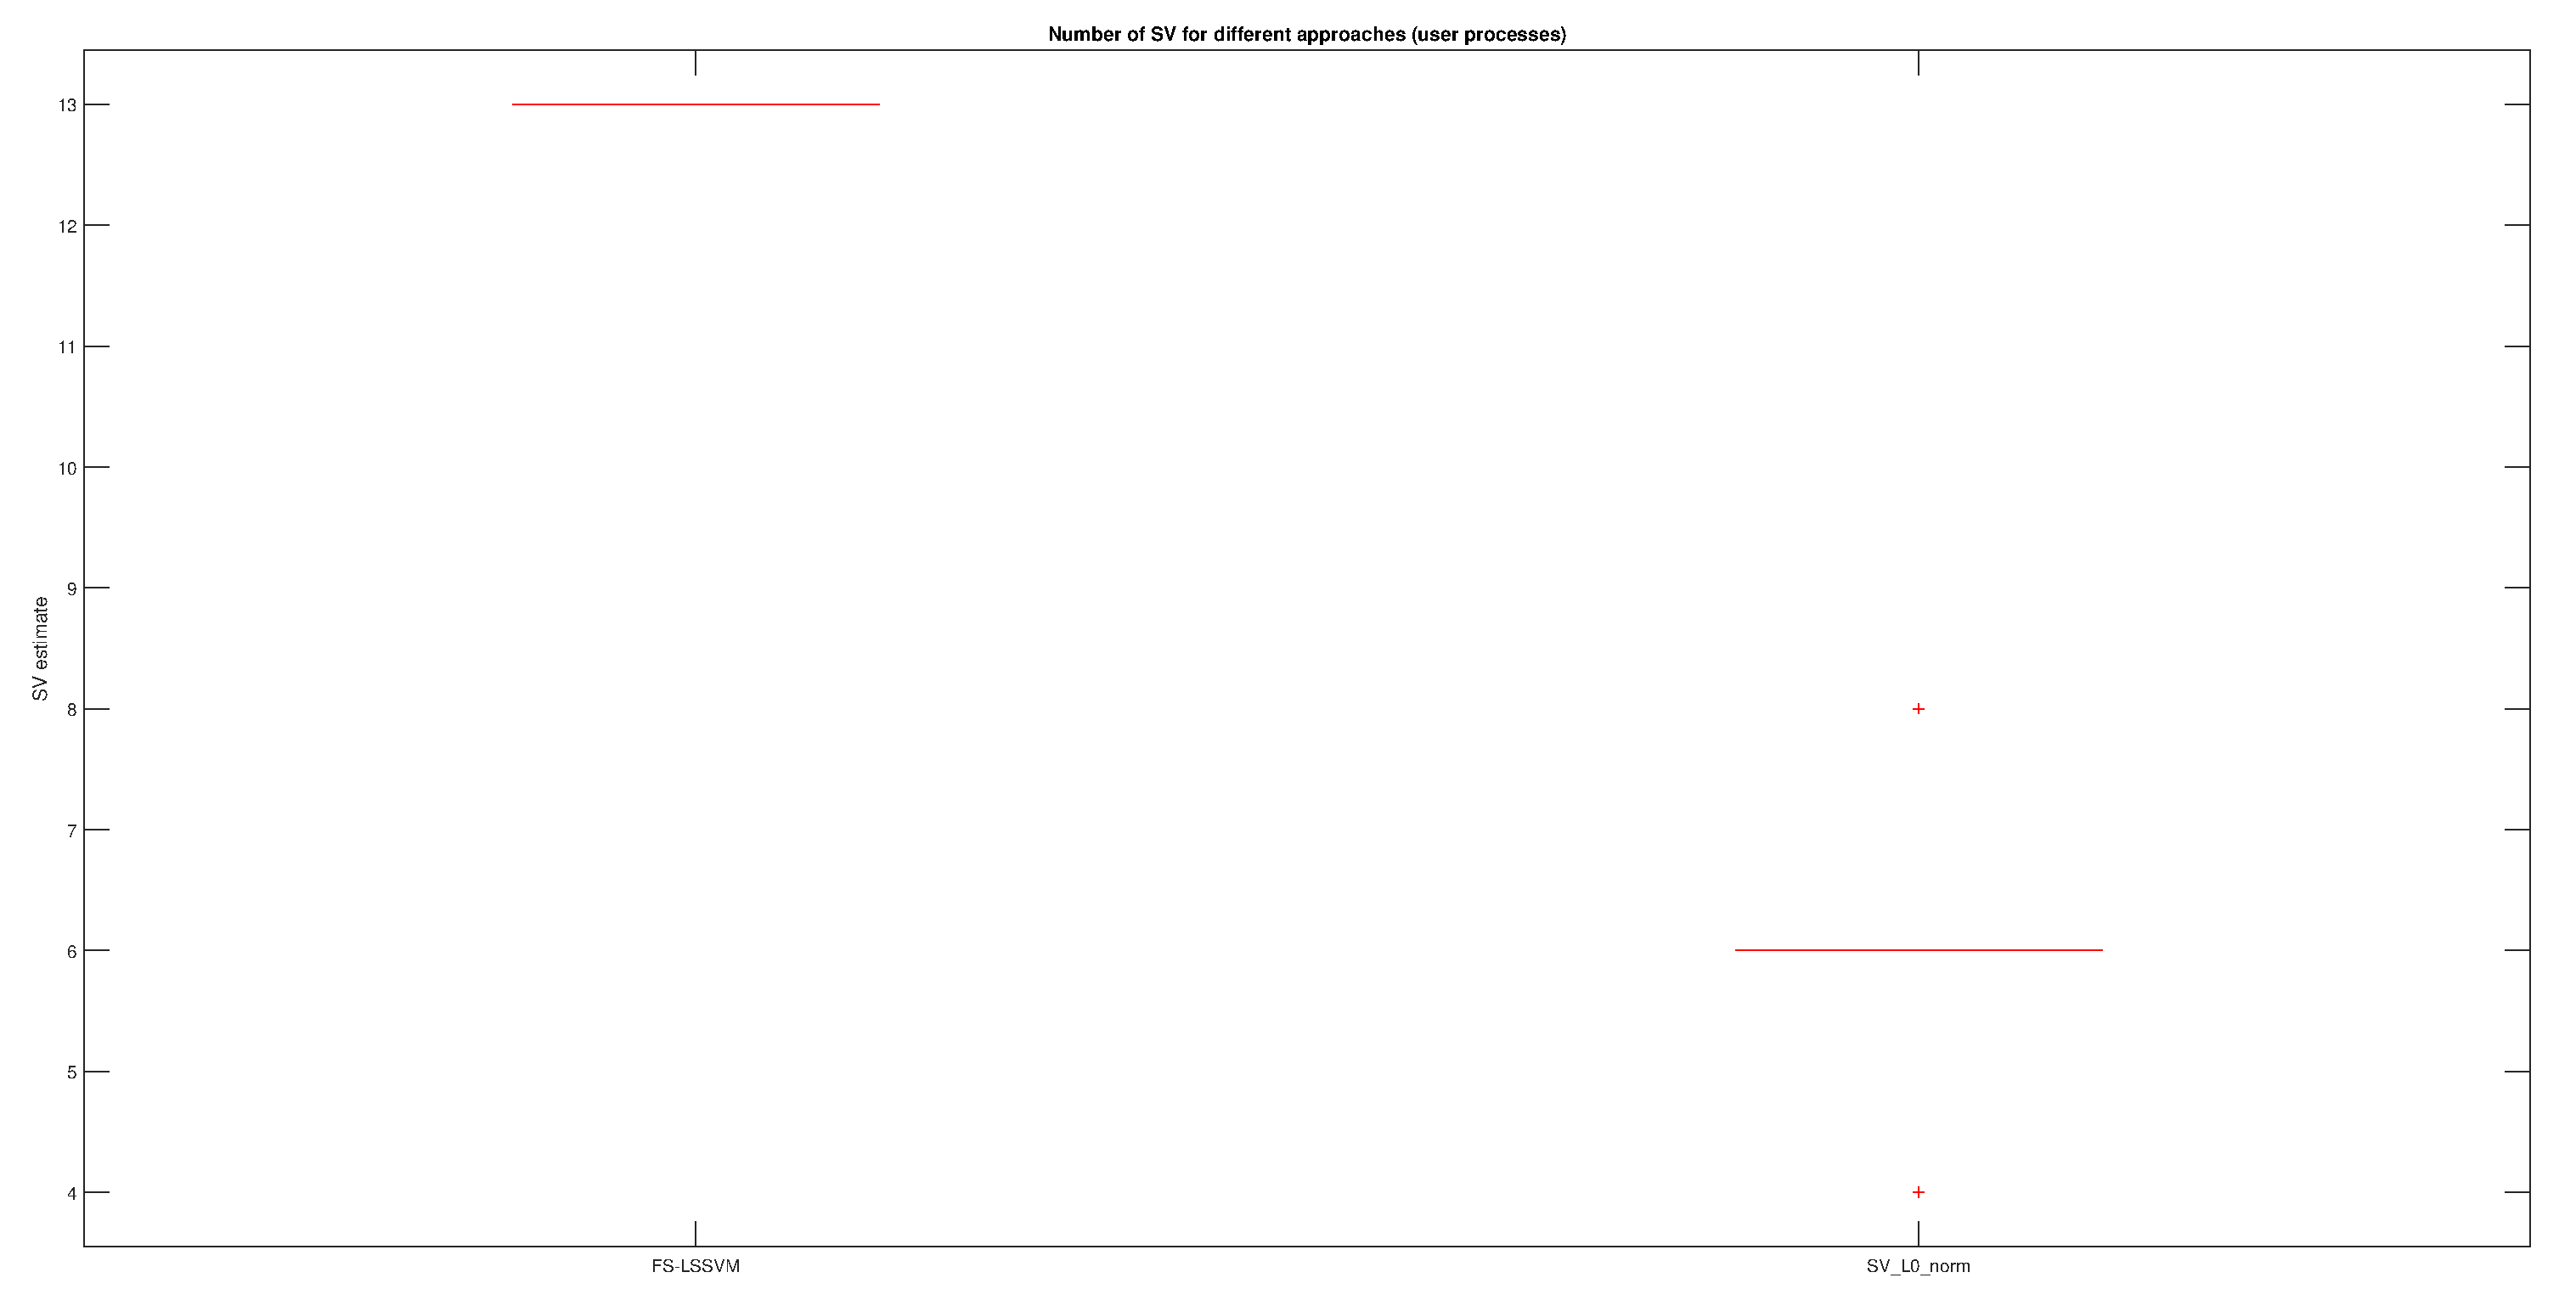
\includegraphics[height= 0.65\textwidth, width = 0.8\textwidth]{Exercise3/Report/shuttle_2}
		\caption{Number of Support Vectors}\label{fig:shuttle_2}
	\end{subfigure}%
	\begin{subfigure}[b]{0.34\textwidth}
		\centering
		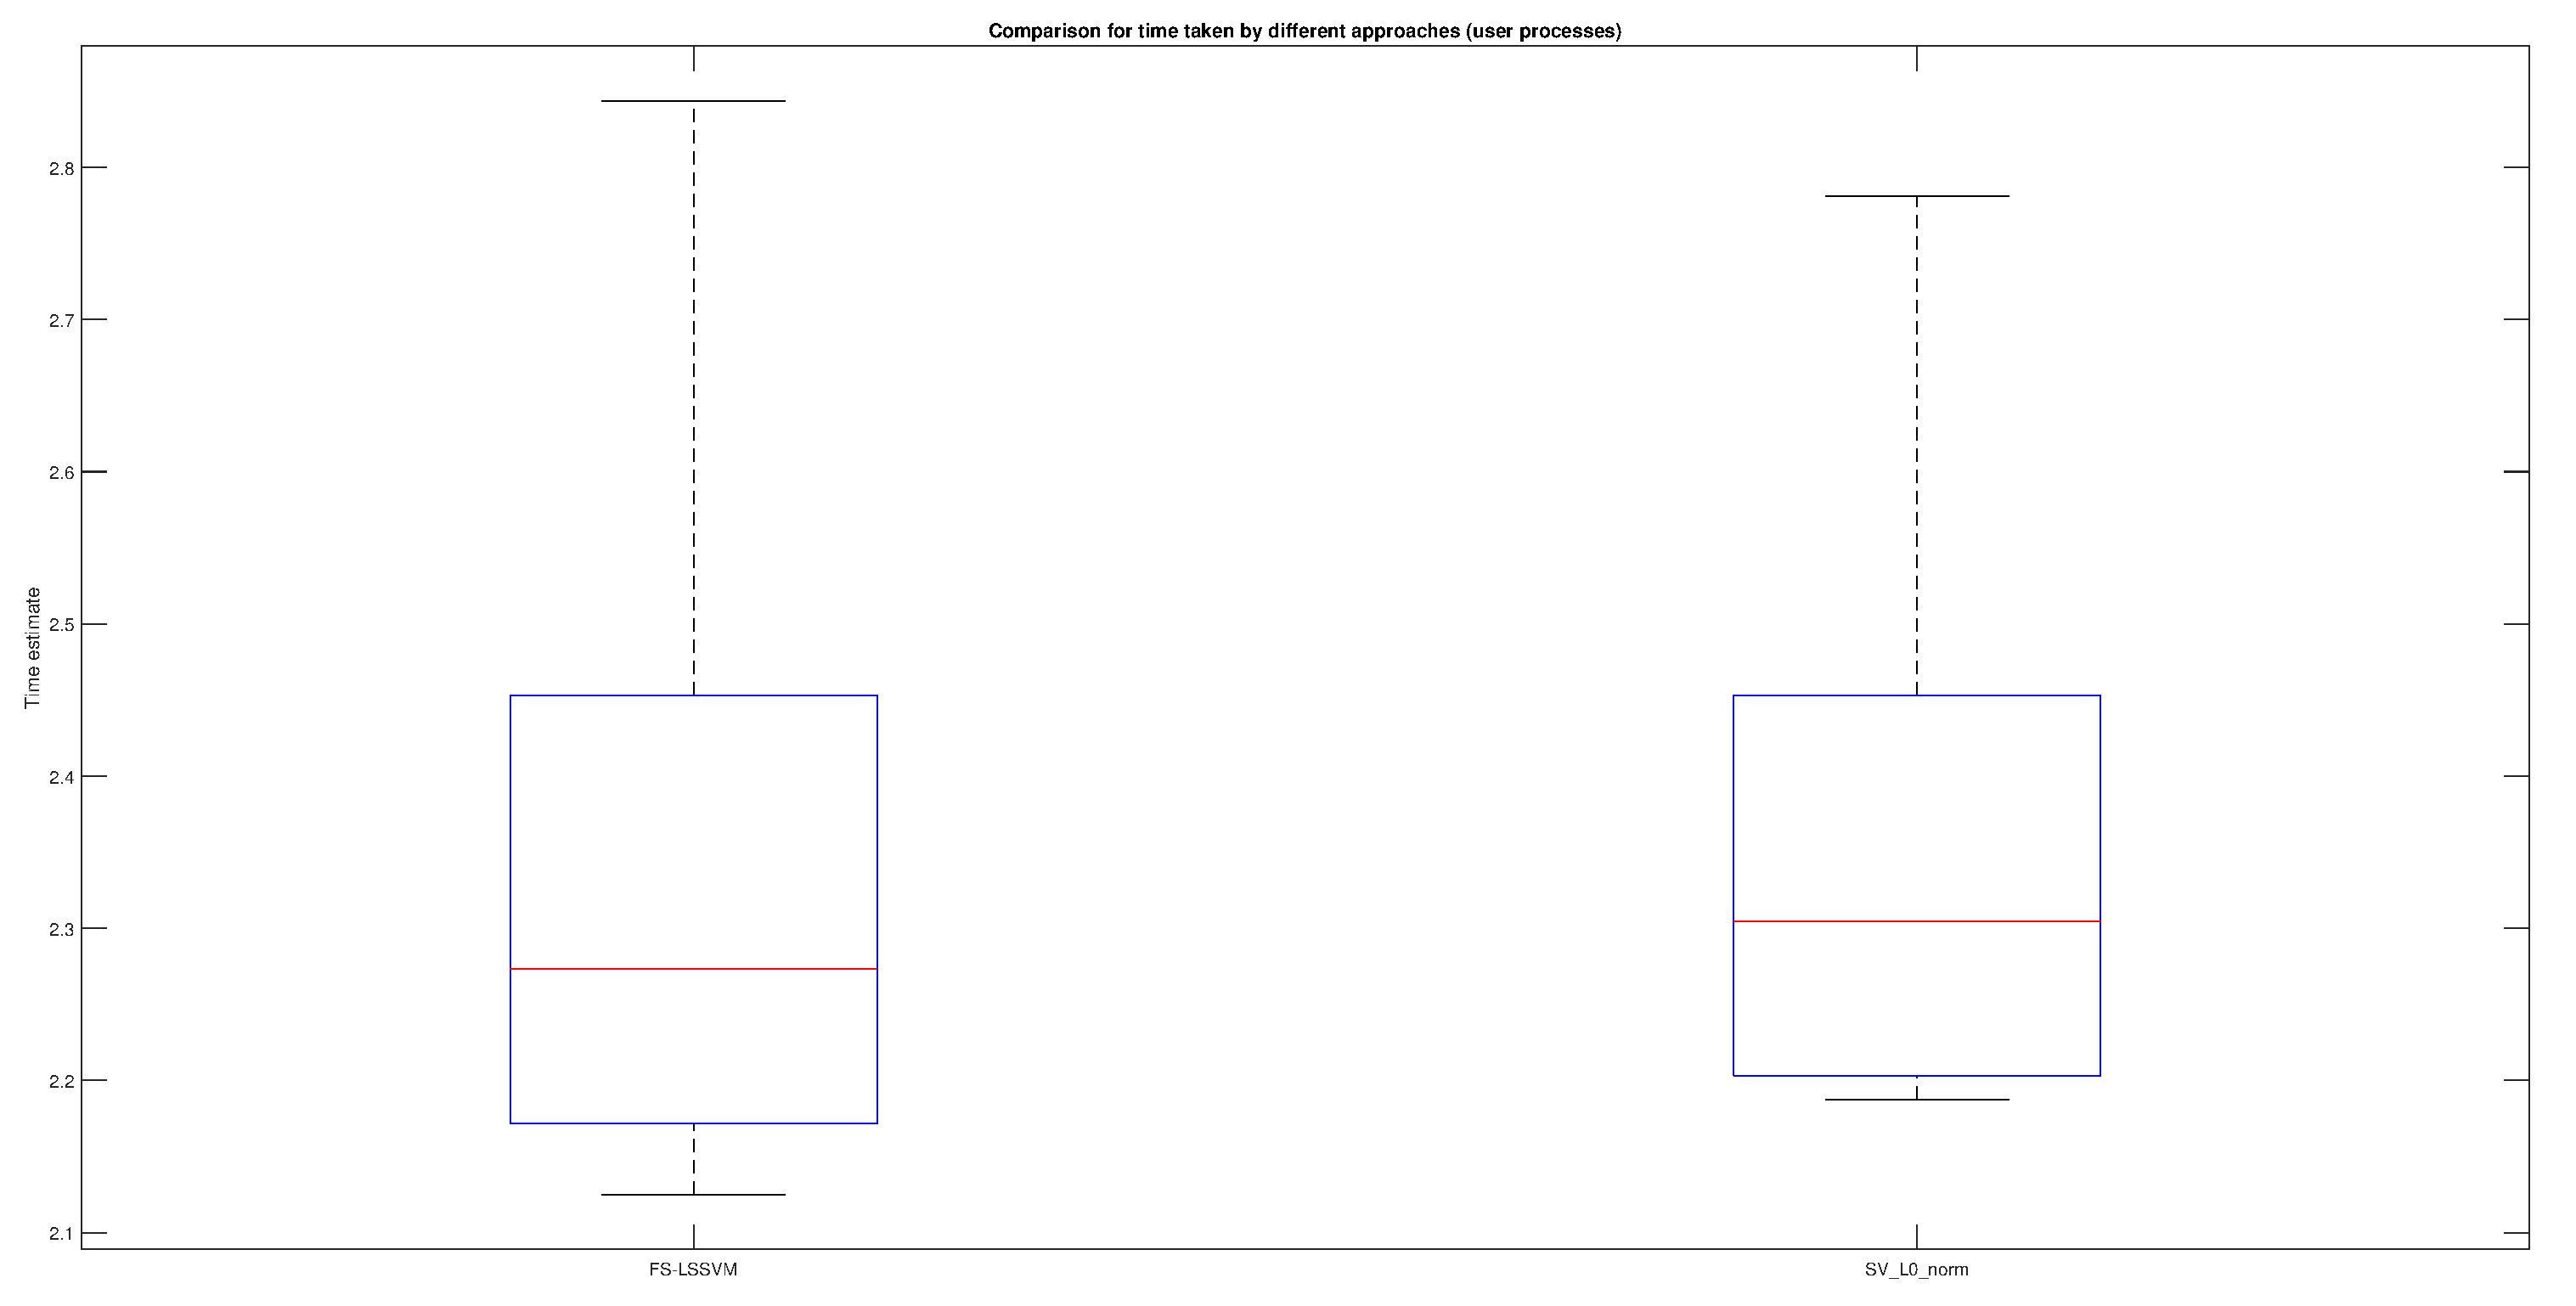
\includegraphics[height= 0.65\textwidth, width = 0.8\textwidth]{Exercise3/Report/shuttle_3}
		\caption{Computation Time}\label{fig:shuttle_3}
	\end{subfigure}%
	\caption{Shuttle Dataset; Fixed Size - LSSVM vs $l_0$ - type approximation}
	\label{fig:shuttle}
\end{figure}

\subsubsection{ California dataset}
The California log dataset contains 20.640 data points with 9 different features. Fixed-size LS-SVM algorithm is run on this dataset and the results are plotted in the below figure \ref{fig:cali}. The error estimates is almost same for both the methods but Fixed-size LSSVM is has slight lower error by a value of 0.001 with no variability. Both FS-LSSVM and $l_0$ type methods takes equal number of support vectors around 42  as seen from figure \ref{fig:cali_2}. Also both methods takes same computational time as seen from figure \ref{fig:cali_3}. 
\begin{figure}[!htpb]
	\begin{subfigure}[b]{0.34\textwidth}
		\centering
		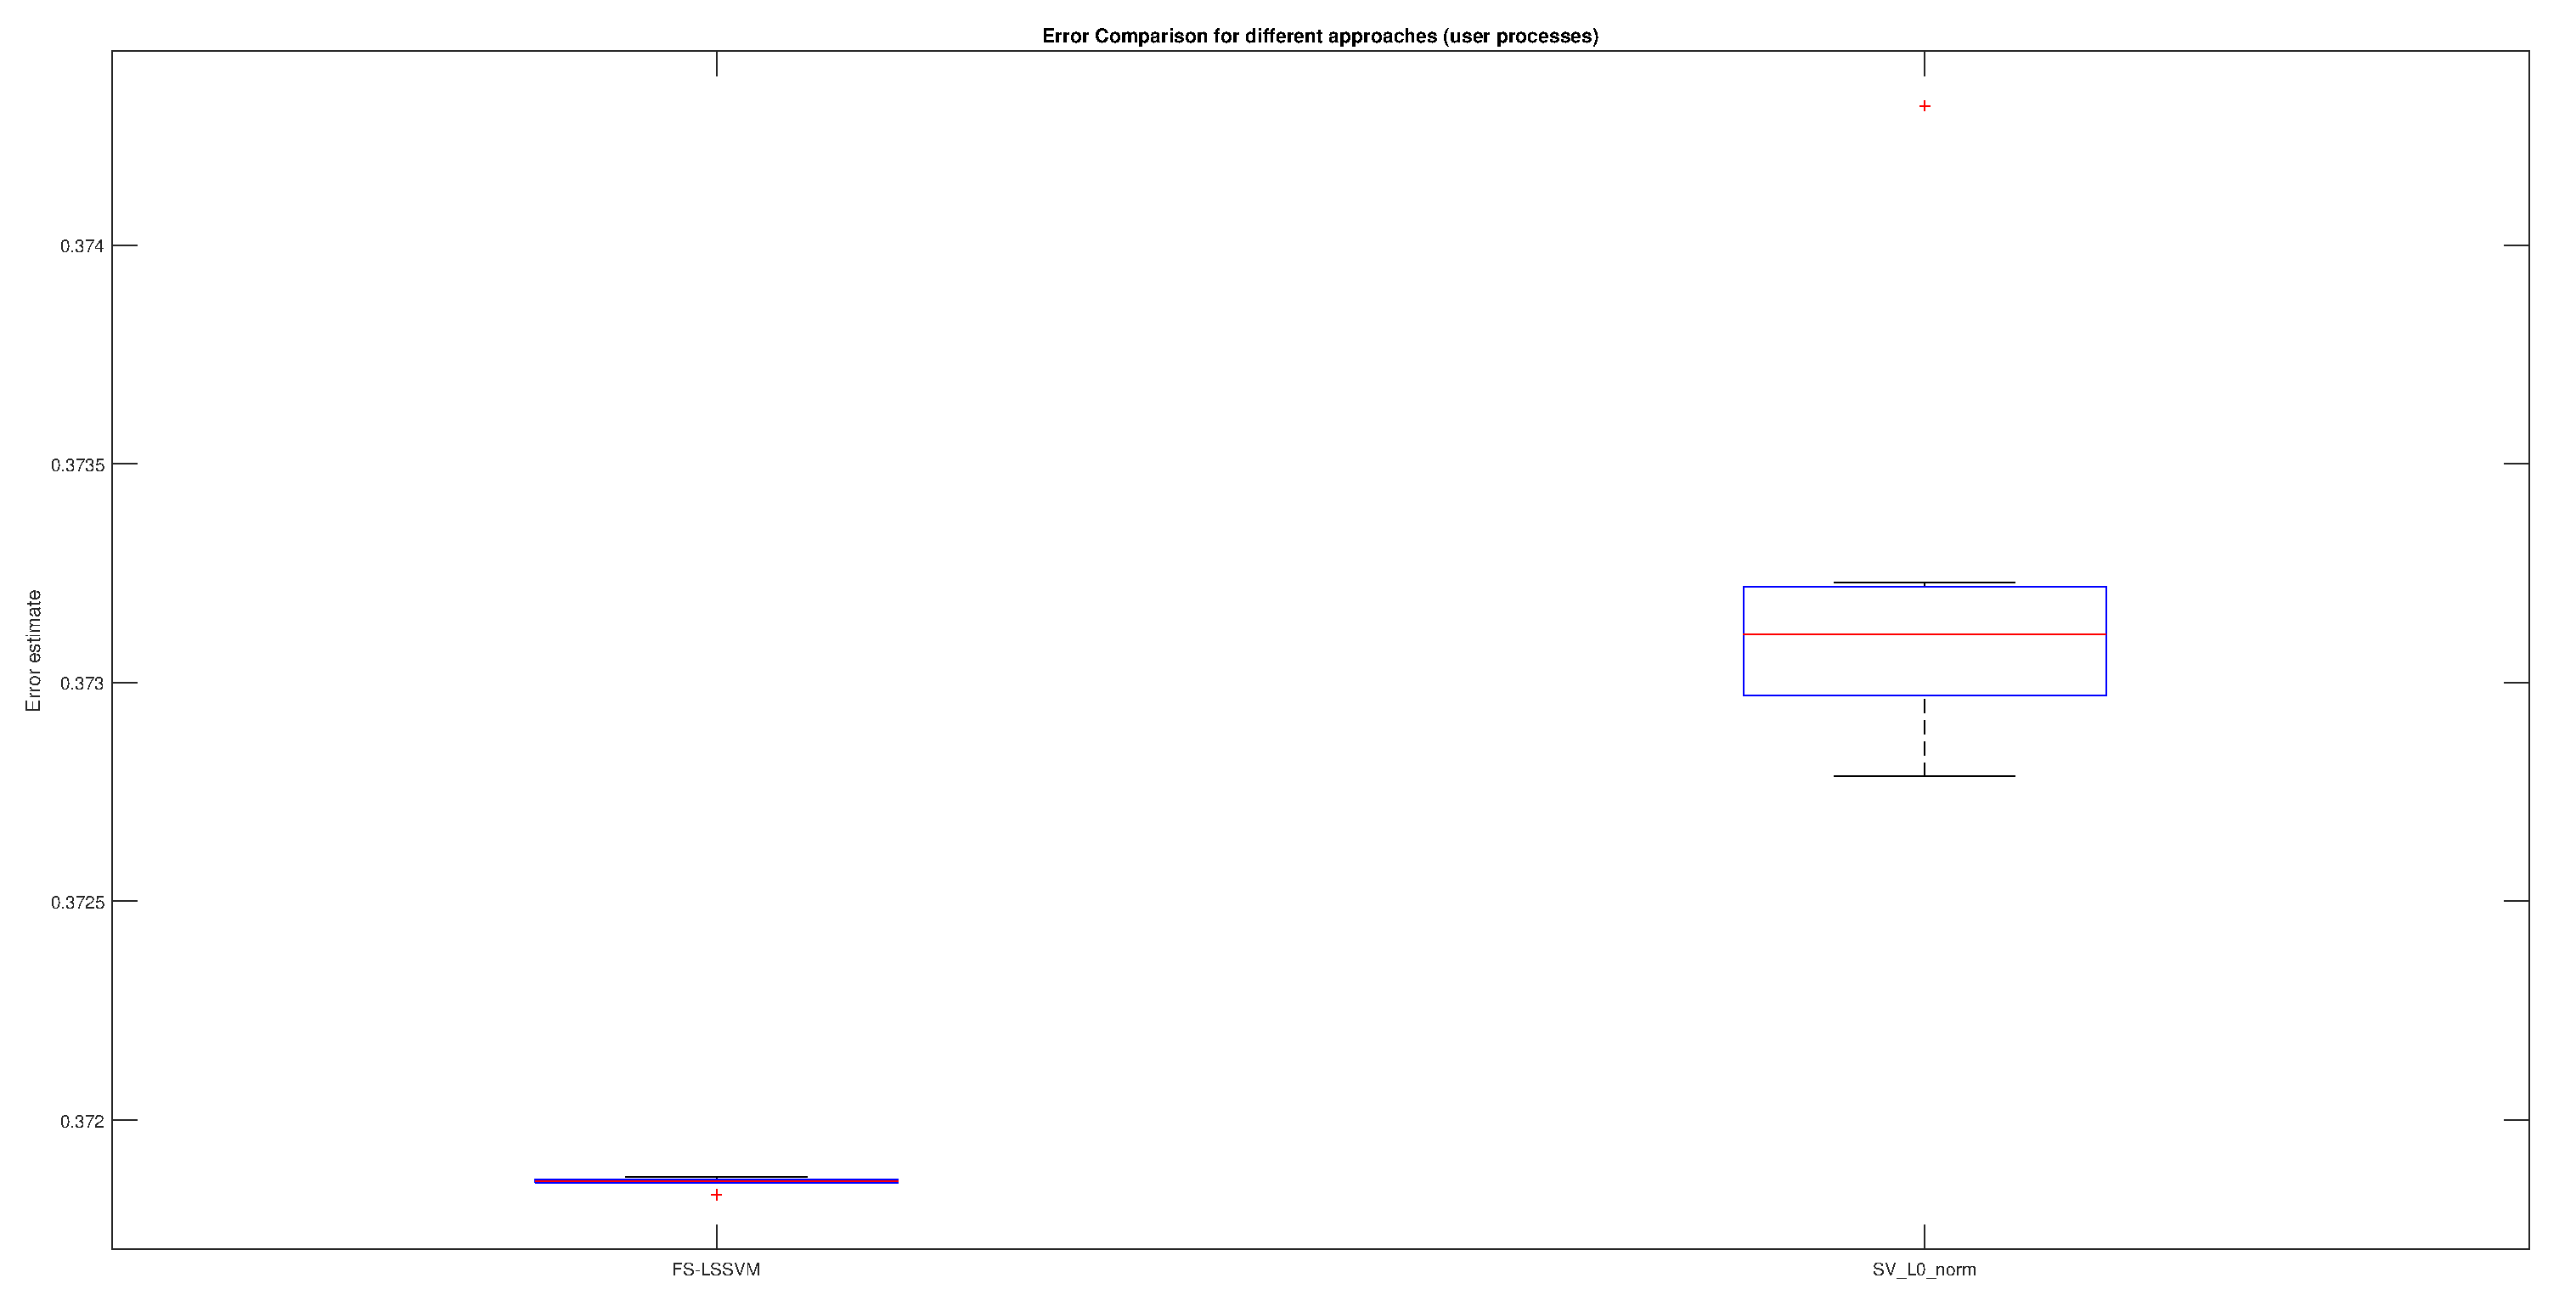
\includegraphics[height= 0.65\textwidth, width = 0.8\textwidth]{Exercise3/Report/cali_1}
		\caption{Error estimates }\label{fig:cali_1}
	\end{subfigure}%
	\begin{subfigure}[b]{0.34\textwidth}
		\centering
		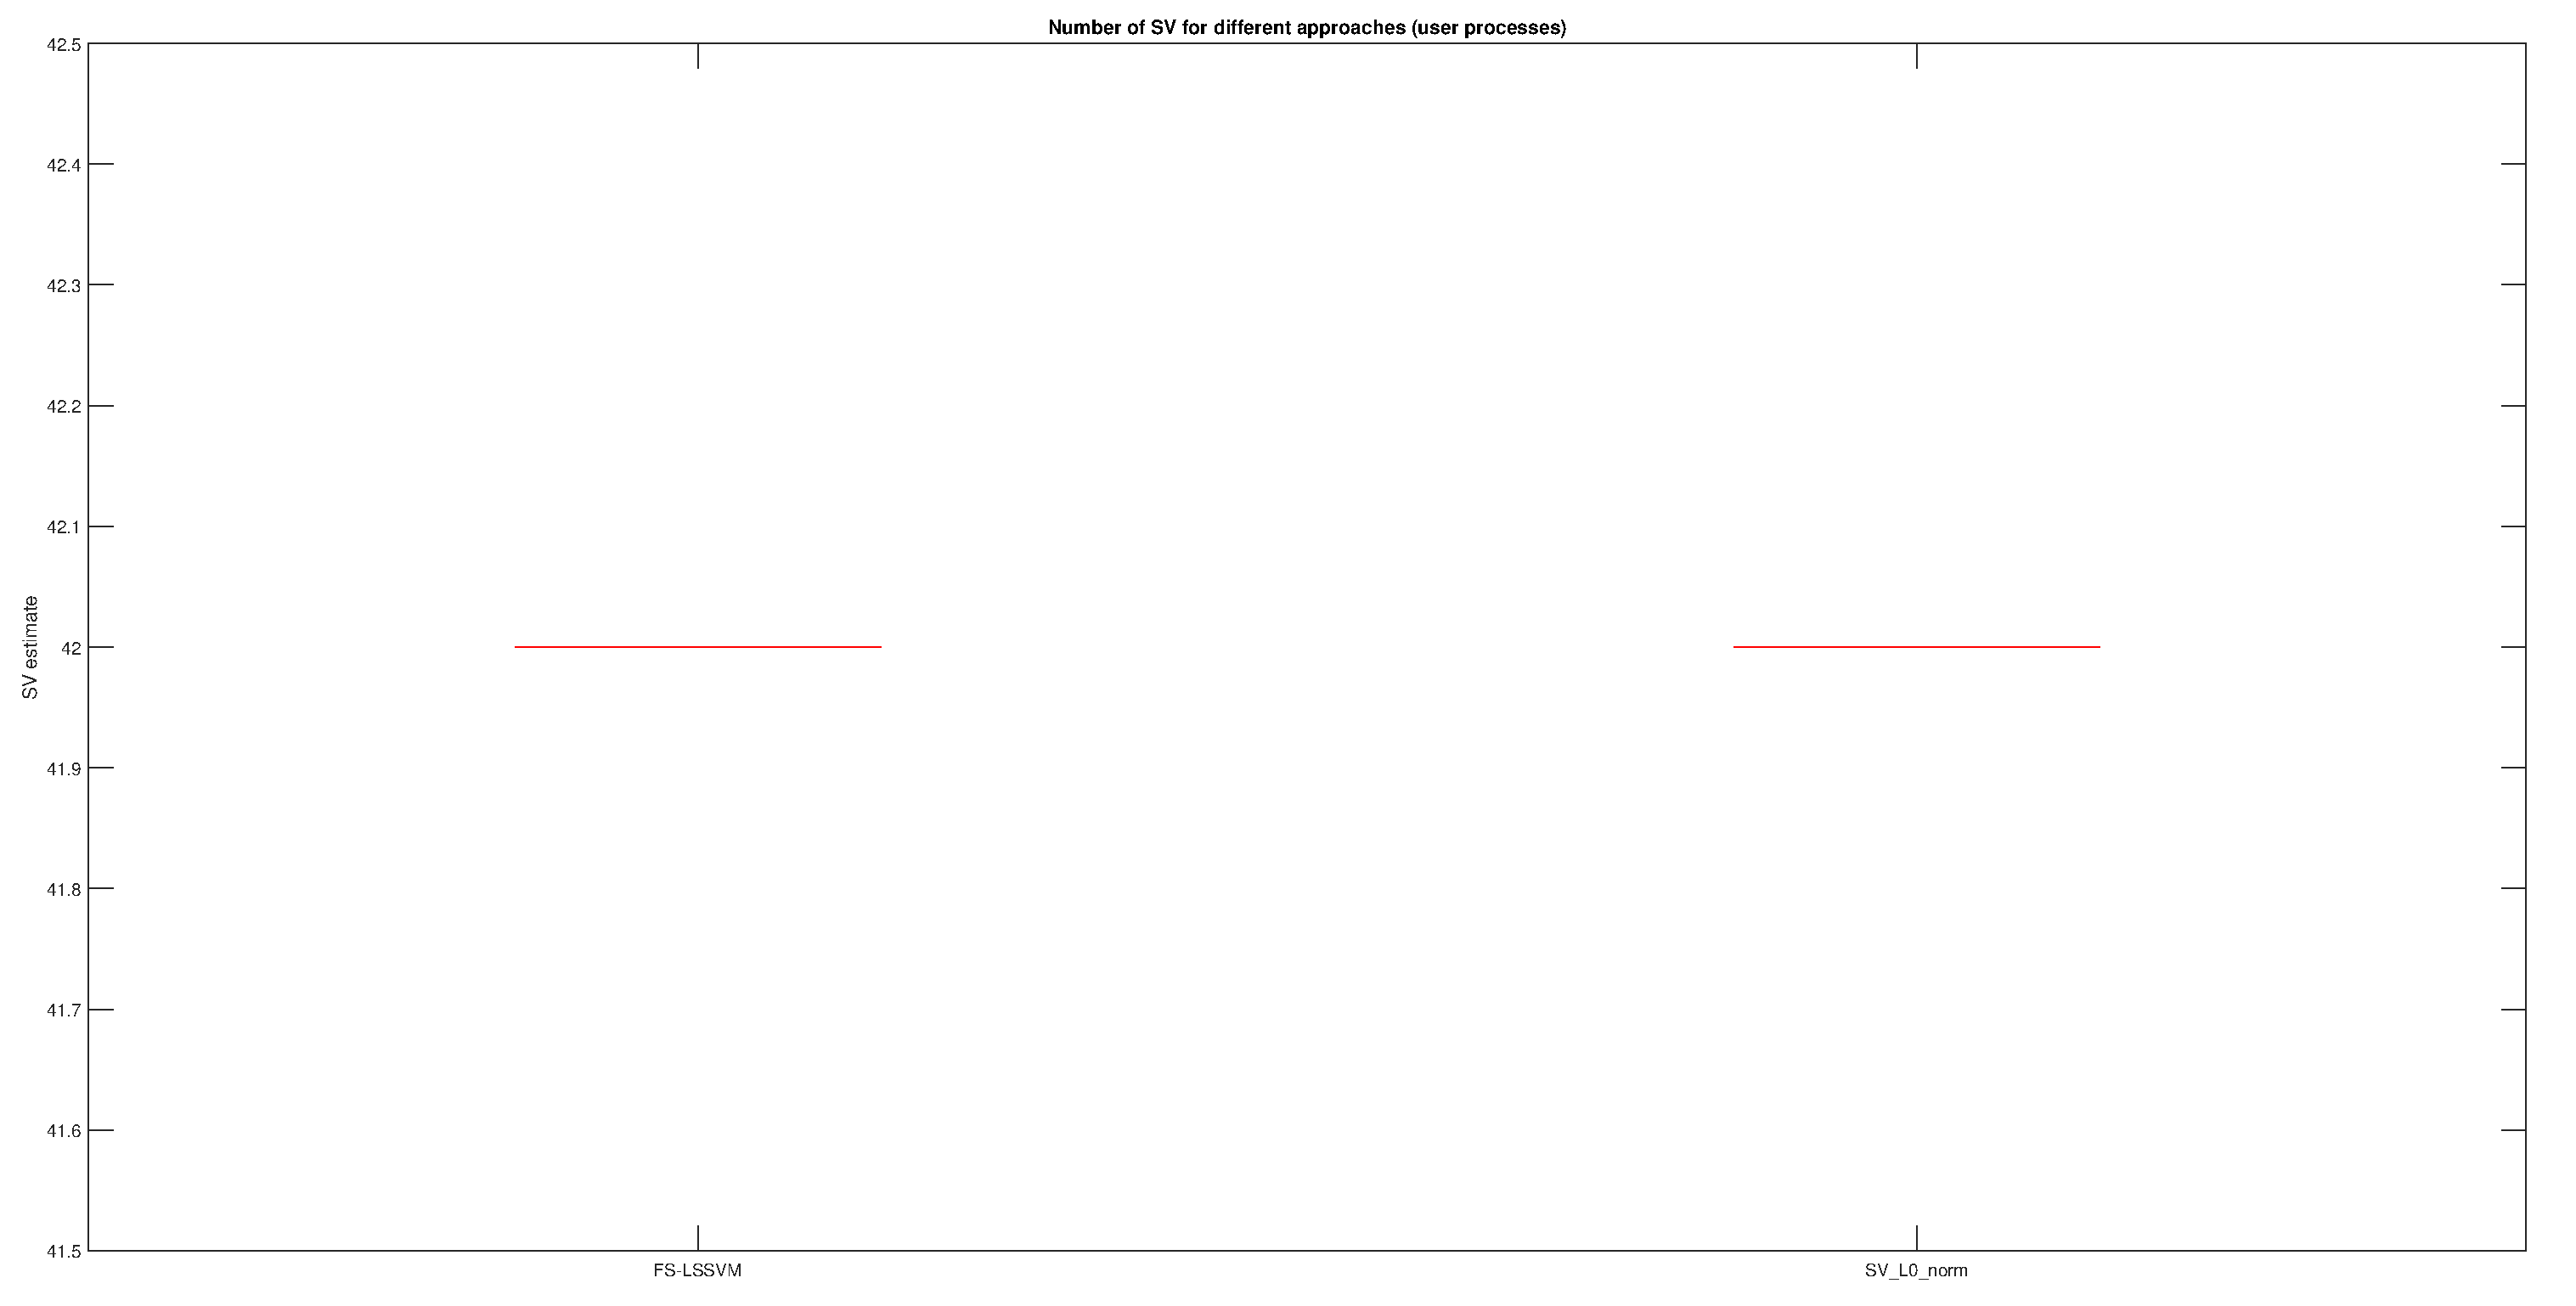
\includegraphics[height= 0.65\textwidth, width = 0.8\textwidth]{Exercise3/Report/cali_2}
		\caption{Number of Support Vectors}\label{fig:cali_2}
	\end{subfigure}%
	\begin{subfigure}[b]{0.34\textwidth}
		\centering
		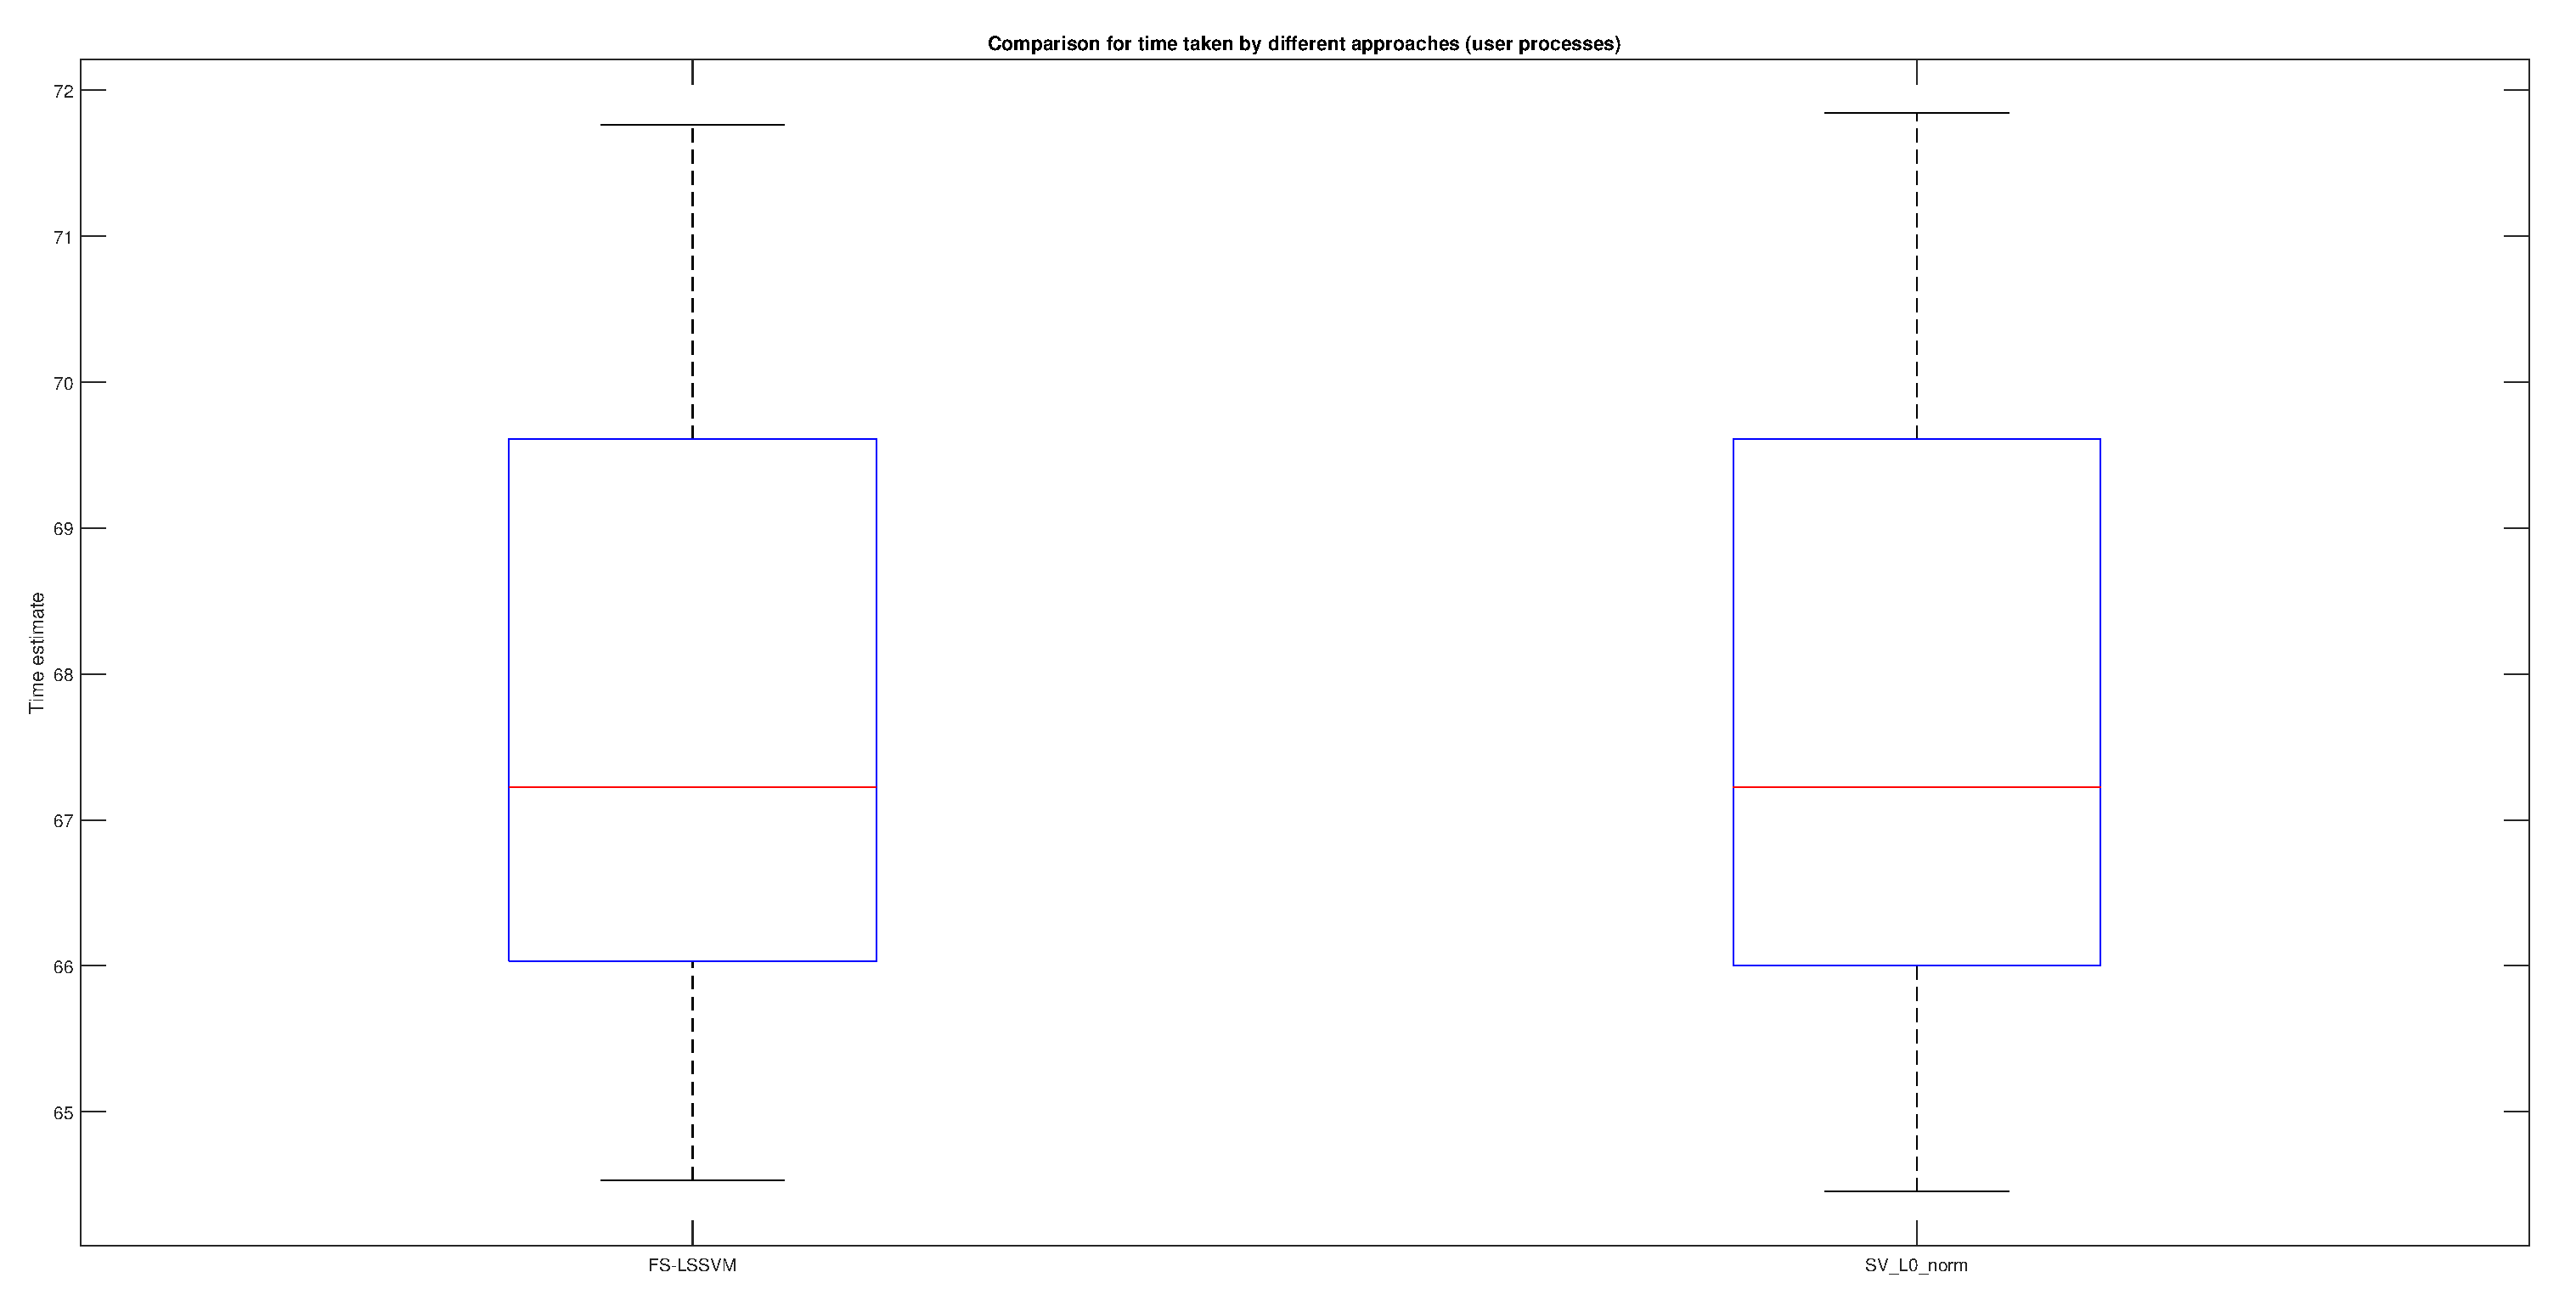
\includegraphics[height= 0.65\textwidth, width = 0.8\textwidth]{Exercise3/Report/cali_3}
		\caption{Computation Time}\label{fig:cali_3}
	\end{subfigure}%
	\caption{California Dataset; Fixed Size - LSSVM vs $l_0$ - type approximation}
	\label{fig:cali}
\end{figure}